%                                     MMMMMMMMM        
%                                                                             
%  MMO    MM   MMMMMM  MMMMMMM   MM    MMMMMMMM   MMD   MM  MMMMMMM MMMMMMM   
%  MMM   MMM   MM        MM     ?MMM              MMM$  MM  MM         MM     
%  MMMM 7MMM   MM        MM     MM8M    MMMMMMM   MMMMD MM  MM         MM     
%  MM MMMMMM   MMMMMM    MM    MM  MM             MM MMDMM  MMMMMM     MM     
%  MM  MM MM   MM        MM    MMMMMM             MM  MMMM  MM         MM     
%  MM     MM   MMMMMM    MM   MM    MM            MM   MMM  MMMMMMM    MM
%
%
%            - META-NET Language White Paper | Slovak content -
% 
% ----------------------------------------------------------------------------

\begin{document}

\maketitle

% --------------------------------------------------------------------------
% Preface
\bsection*{Predhovor --- Preface}

\null
\pagestyle{empty} 

\pagenumbering{Roman} 
\setcounter{page}{3}
\pagestyle{scrheadings}

\begin{Parallel}[c]{78mm}{78mm}
\ParallelLText{\selectlanguage{slovak}
Táto biela kniha je súčasťou série, ktorá propaguje najnovšie poznatky
a~potenciál jazykových technológií. Je určená novinárom, politikom, jazykovým spoločnostiam, učiteľom a iným. V~európskych krajinách majú jazykové technológie rozličnú úroveň aj využitie. Z~toho dôvodu sú aj opatrenia potrebné na ďalšiu podporu výskumu a~vývoja jazykových technológií pre každý jazyk odlišné. Požadované opatrenia závisia od mnohých faktorov, akými sú napríklad zložitosť daného jazyka či veľkosť jazykovej komunity.

META-NET, sieť excelentnosti, financovaná z~fondov Európskej komisie,
vypracovala v tejto sérii bielych kníh (s.~\pageref{whitepaperseries}) analýzu súčasných jazykových zdrojov a~technológií. Analýza zahŕňala okrem 23 oficiálnych
európskych jazykov aj iné dôležité národné i~regionálne jazyky Európy. Výsledky analýzy poukázali na značné nedostatky v technologickej podpore a na medzery vo výskume pre~každý jazyk. Podrobnejšia expertná analýza a~zhodnotenie momentálnej situácie pomôže maximalizovať efektivitu ďalších výskumov.

Od novembra 2011 META-NET pozostáva z~54 výskumných centier v~33 krajinách Európy (s.~\pageref{metanetmembers}). META-NET spolupracuje so zainteresovanými stranami
z~oblasti ekonómie (softvérové spoločnosti, poskytovatelia technológií a používatelia), z oblasti vládnych agentúr, výskumných organizácií, nevládnych organizácií, jazykových spoločenstiev a~európskych univerzít. META-NET spoločne s týmito komunitami vytvára jednotnú technologickú víziu a strategický plán výskumu pre multilingválnu Európu 2020.}

\ParallelRText{\selectlanguage{english}

This white paper is part of a series that promotes knowledge about language technology and its potential. It addresses journalists, politicians, language communities, educators and others. 
The availability and use of language technology in Europe varies between languages. Consequently, the actions that are required to further support research and development of language technologies also differ. The required actions depend on many factors, such as the complexity of a given language and the size of its community.

%META-NET, a Network of Excellence funded by the European Commission, has conducted an analysis of current language resources and technologies. This analysis focused on the 23 official European languages as well as other important national and regional languages in Europe. The results of this analysis suggest that there are many significant research gaps for each language. A more detailed expert analysis and assessment of the current situation will help maximise the impact of additional research and minimise any risks.
META-NET, a Network of Excellence funded by the European Commission, has conducted an  analysis of current language resources and technologies in this white paper series (p.~\pageref{whitepaperseries}). The analysis focuses on the 23 official European languages as well as other important national and regional languages in Europe. The results of this analysis suggest that there are tremendous deficits in technology support and significant research gaps for each language. The given detailed expert analysis and assessment of the current situation will help maximise the impact of future research.

%META-NET consists of 54 research centres from 33 countries that are working with stakeholders from commercial businesses, government agencies, industry, research organisations, software companies, technology providers and European universities. Together, they are creating a common technology vision while developing a strategic research agenda that shows how language technology applications can address any research gaps by 2020.}
As of November 2011, META-NET consists of 54 research centres in 33 European countries (p.~\pageref{metanetmembers}). META-NET is working with stakeholders from economy (software companies, technology providers and users), government agencies, research organisations, non-governmental organisations, language communities and European universities. Together with these communities, META-NET is creating a common technology vision and strategic research agenda for multilingual Europe 2020.} 
\ParallelPar
\end{Parallel}

\makefundingnotice

\cleardoublepage
% --------------------------------------------------------------------------
% Table of Contents
\bsection*{Obsah --- Contents}

\tableofcontents

\addtocontents{toc}{\protect\thispagestyle{empty}\protect}
\addtocontents{toc}{{\Large\textsf{\centerline{SLOVENSKÝ JAZYK V DIGITÁLNOM VEKU}}\par}}

\cleardoublepage

\setcounter{page}{1}
\pagenumbering{arabic} 
\pagestyle{scrheadings}
% --------------------------------------------------------------------------
% Start of original language part
\selectlanguage{slovak}

% Chapter 1
\ssection[Zhrnutie]{Zhrnutie}
\begin{multicols}{2}
Európa sa počas posledných 60 rokov stala výraznou politickou
a~ekonomickou štruktúrou, ale kultúrne a~jazykovo je stále
veľmi rôznorodá. To znamená, že od Portugalska po Poľsko
a~od Talianska po Island je bežná komunikácia medzi občanmi Európy podobne ako komunikácia v~oblasti podnikania a~politiky neustále konfrontovaná s~jazykovými bariérami. Európske inštitúcie minú ročne približne miliardu eur na preklady inojazyčných textov a~na tlmočenie. Nemuselo by to tak byť, ak by moderné jazykové technológie a~lingvistický výskum pomohli prekonať jazykové hranice. Ak vhodne využijeme inteligentné zariadenia a~aplikácie, budeme môcť vzájomne diskutovať alebo obchodovať a~rozličné jazyky nebudú pre nás prekážkou.

\boxtext{Jazykové technológie predstavujú mosty}

Jedným zo spôsobov, ako prekonať jazykové bariéry, je naučiť sa
niekoľko cudzích jazykov. Zvládnuť 23 oficiálnych jazykov
členských štátov EÚ a~približne 60 ďalších európskych jazykov
je málo pravdepodobné. Vďaka technologickej podpore však dokážeme
viesť politické aj ekonomické rokovania, ako aj napredovať vo
výskume.

Riešením mnohojazyčnosti je vybudovanie kľúčových technológií,
ktoré európskym činiteľom ponúknu obrovské výhody, a~to nielen
v~rámci spoločného európskeho trhu, ale aj pri obchodných vzťahoch
s~krajinami  tretieho sveta, najmä s~krajinami rozvíjajúcej sa
ekonomiky. Aby sme dosiahli tento cieľ a~zároveň zachovali kultúrnu
a~jazykovú rozmanitosť, musíme systematicky analyzovať špecifiká
všetkých európskych jazykov, ako aj stav súčasných jazykových
technológií. Navrhnuté riešenia budú mostom medzi jazykmi.

Automatické preklady a~nástroje na spracovanie reči
v~súčasnosti nedosahujú svoje ciele v~dostatočnej miere. V~tomto
odvetví sú dominantné najmä súkromné podniky zo Severnej Ameriky.
Na konci 70. rokov si Európa začala uvedomovať hlboký význam
jazykových technológií pre integráciu Európy a~začala podporovať
prvé výskumné projekty, napr. projekt EUROTRA. Zároveň sa
realizovali viaceré národné projekty s~hodnotnými výsledkami,
ktoré sa však výraznejšie do európskeho povedomia nedostali.
V~iných jazykových spoločenstvách, napr. v~Indii s~22 úradnými
jazykmi a~v~Južnej Afrike s~11 úradnými jazykmi, sa predsa len
podarilo vybudovať dlhodobé národné programy na výskum a~rozvoj
jazykových technológií.
Hlavní hráči v oblasti jazykových technológií v~súčasnosti
používajú nepresné štatistické prístupy, ktoré nevyužívajú
hlbšie lingvistické metódy a znalosti.
Napríklad pri automatickom preklade sa vety 
prekladajú porovnávaním novej vety s~tisíckami iných viet, ktoré
predtým už niekto preložil. Preto kvalita závisí do značnej miery
od~množstva a~kvality týchto prekladov v~korpuse.

\boxtext{Jazykové technológie sú kľúčom do budúcnosti}

Automatický preklad
jednoduchých viet akéhokoľvek jazyka, pre ktorý máme dostatočné
množstvo textového materiálu, dosahuje dobré výsledky, ale takéto
štatistické metódy zlyhávajú pre jazyky s menším množstvom zdrojového materiálu.

Európska únia sa preto od roku 2006 rozhodla financovať projekty, ako
je EuroMatrix alebo EuroMatrixPlus a~od roku 2010 aj iTranslate4, ktoré
vykonávajú základný aj~aplikovaný výskum a~zhromažďujú zdroje,
ktoré by pre všetky európske jazyky stanovili sofistikované
riešenia jazykových technológií. Aby sme vybudovali kvalitné
aplikácie, je nevyhnutné detailnejšie preskúmať štruktúru jazyka.

Európsky výskum v~tejto oblasti už dosiahol svoje úspechy.
Napríklad EÚ používa na prekladateľské služby prekladový
softvér MOSES, ktorý bol vyvinutý vďaka viacerým európskym
výskumným projektom. Jeden z~nich, projekt Verbmobil, ktorý
financovalo ministerstvo školstva a~výskumu v~Nemecku, mal vo sfére
prekladu reči na istý čas vedúcu pozíciu. Mnohé z~výskumných
laboratórií boli, bohužiaľ, zrušené, príp. presunuté, čoho
dôsledkom je tendencia v~Európe rozvíjať výskumnú činnosť
v~izolácii, a~teda so~slabším prienikom na~svetový trh.

Na základe súčasných poznatkov sa zdá, že dnešné „hybridné“ jazykové technológie, ktoré využívajú štatistické prístupy, by mohli prekonať jazykovú priepasť v~rámci Európy aj mimo nej. Séria bielych kníh poukazuje na značné rozdiely medzi jazykmi v~stave jazykových technológií. Aj slovenský jazyk potrebuje mimoriadne efektívne riešenia na ďalší výskum a~rozvoj jazykových technológií.

\boxtext{Jazykové technológie pomáhajú zjednotiť Európu}

Dlhodobým cieľom META-NET-u je pos\-kyt\-núť kvalitné jazykové technológie všetkým jazykom, aby sa zároveň dosiahla politická a~ekonomická jednota napriek kultúrnym rozdielom. Technologické nástroje pomôžu prekonať existujúce bariéry. Všetky zainteresované strany (z~oblasti politiky, vedy, obchodu a~pod.) by sa mali snažiť o~zjednotenie.

Táto séria bielych kníh dopĺňa aj ďalšie aktivity META-NET-u (pozri prílohu). Aktuálne informácie, napríklad najnovšie vízie alebo strategický výskumný program META-NET-u sú dostupné na oficiálnej webovej stránke META-NET-u: \url{http://www.meta-net.eu}.
\end{multicols}

\clearpage

% Chapter 2
\ssection[Ohrozenie našich jazykov: Výzva pre jazykové technológie]{Ohrozenie našich jazykov: Výzva pre jazykové technológie}

\begin{multicols}{2}

V~poslednej dekáde sme svedkami digitálnej revolúcie, ktorá má značný vplyv na komunikáciu a~spoločnosť. Nedávne pokroky v~digitálnych a~sieťových komunikačných technológiách sa niekedy prirovnávajú ku Gutenbergovmu vynájdeniu kníhtlače. Ako nám môže táto analógia konkrétne priblížiť budúcnosť európskej informačnej spoločnosti a~našich jazykov?

\boxtext{Sme svedkami digitálnej revolúcie, ktorú môžeme prirovnať
ku Gutenbergovmu vynálezu kníhtlače}

Po Gutenbergovom vynáleze nastal skutočný prelom v~komunikácii
a~výmene poznatkov vďaka takým snahám, ako bol napr. Lutherov
preklad Biblie do zrozumiteľného jazyka. V~ďalších storočiach
nastal rozvoj kultúrnych postupov, ktoré rozšírili
výmenu poznatkov a~zefektívnili spracovávanie jazyka. Zmeny,
ktoré nastali:

\begin{itemize}
\item ortografické a~gramatické ustálenie významnejších jazykov umožnilo rýchle rozšírenie nových vedeckých a~intelektuálnych ideí;
\item rozvoj oficiálnych jazykov pomohol obyvateľom komunikovať v~rámci určitých (často politických) hraníc;
\item vyučovanie a~preklad jazykov umožnil výmenu poznatkov medzi jazykmi;
\item vytvorenie žurnalistických a~bibliografických príručiek prinieslo zlepšenie kvality a~dostupnosti tlačeného materiálu;
\item vytvorenie rôznych médií, akými sú knihy, noviny, rozhlas, televízia a~i. uspokojilo rozmanité komunikačné potreby.
\end{itemize}

Za posledných dvadsať rokov pomohli informačné technológie automatizovať a~uľahčiť celý rad procesov:

\begin{itemize}
\item DTP softvér nahradil strojopis a~sadzbu;
\item prezentačný softvér, ako napríklad OpenOffice/LibreOffice Impress alebo Microsoft PowerPoint nahradili spätný projektor;
\item zasielanie a~prijímanie dokumentov e-mailom je rýchlejšie ako prostredníctvom faxu;
\item SIP telefónia alebo Skype umožňujú internetové volania a~virtuálne stretnutia;
\item efektívne kódovanie zvukových a~obrazových súborov uľahčuje výmenu multimediálneho obsahu;
\item nástroje na vyhľadávanie umožňujú na báze kľúčových slov efektívny prístup na webové stránky;
\item on-line služby, ako napríklad Google Translate, ponúkajú rýchle, aj keď približné preklady;
\item platformy sociálnych médií (Pokec, Facebook, Twitter, Google a~i.) uľahčujú spoluprácu a~sprístupnenie informácií.
\end{itemize}

Spomenuté nástroje a~aplikácie ľuďom pomáhajú, no v~súčasnosti nedokážu dostatočne pokryť potreby multilingválnej modernej európskej informačnej spoločnosti, v~ktorej je neustály tok informácií a~tovaru.

\subsection{Jazykové hranice spomaľujú európsku informačnú spoločnosť}
V~súčasnosti nemôžeme presne odhadnúť, aká bude informačná
spoločnosť o~niekoľko rokov. Je však veľmi pravdepodobné, že
revolúcia v~komunikačných technológiách spojí ľudí, ktorí
hovoria rozličnými jazykmi, napriek jazykovým bariéram. Momentálne
môžeme cítiť istý tlak na ľudí, aby sa učili cudzie jazyky,
a~najmä na ľudí, ktorí by mali vytvárať nové technologické
aplikácie na zabezpečenie vzájomného dorozumenia.
V~aktuálnej globálnej ekonomike a~informačnom priestore sa denne
konfrontujeme s~narastajúcim počtom jazykov, hovoriacimi a~novými
témami. Súčasná popularita sociálnych médií (Wikipedia, Facebook,
Twitter, YouTube, Pokec, Google+) je len špičkou tohto pokrokového
ľadovca.

\boxtext{V globálnej ekonomike a informačnom priestore sa denne konfrontujeme s rôznymi jazykmi, hovoriacimi a novými témami}

Dnes dokážeme prenášať gigabajty textu po celom svete za pár
sekúnd, hoci sú v~jazyku, ktorému nerozumieme. Podľa nedávnej
správy, ktorú vydala Európska komisia, 57~\% používateľov
internetu platí za tovar a~služby v~cudzom jazyku (angličtina je
najbežnejšia, hneď za ňou nasleduje francúzština, nemčina
a~španielčina). 55~\% používateľov číta obsah v~cudzom jazyku,
pričom iba 35~\% používa iný jazyk na písanie e-mailov alebo
posielanie komentárov na webe\cite{EC1}. Pred
niekoľkými rokmi mohla byť angličtina internetová lingua franca,
pretože prevažná väčšina materiálov na webe bola v~angličtine.
Situácia sa však medzičasom modifikovala – rozrástlo sa množstvo
inojazyčného on-line obsahu (najmä~ázijského a~arabského).

Táto digitálna priepasť, ktorá je zapríčinená jazykovými
bariérami, prekvapivo nezískala dostatok pozornosti na verejnosti.
Digitálny svet si kladie naliehavú otázku: „Ktorým európskym
jazykom sa bude dariť v~zosieťovanej informačnej a~znalostnej
spoločnosti a~ktoré zaniknú?“

\subsection{Naše jazyky v~ohrození}
Kníhtlač značne prispela k~výmene informácií v~Európe, ale napomohla tiež zániku mnohých európskych jazykov. V~regionálnych a~menšinových jazykoch sa dokumenty rozmnožovali zriedkakedy. Výsledkom bolo, že mnohé jazyky, ako napríklad rómsky alebo rusínsky, sa zredukovali viacmenej len na ústne podanie, čo obmedzovalo ich kontinuálne osvojenie a~rozšírenie. Bude mať internet podobný vplyv aj na naše jazyky?

\boxtext{Rôznorodosť jazykov v Európe je súčasťou najvzácnejšieho a kultúrneho bohatstva Európy}

Približne 80 jazykov je časťou najvzácnejšieho a~najdôležitejšieho kultúrneho bohatstva Európy. Množstvo európskych jazykov je takisto nevyhnutnou súčasťou jej sociálneho úspechu\cite{EC2}. Zatiaľ čo sa budú populárne jazyky ako angličtina a~španielčina v~rozvíjajúcej sa digitálnej spoločnosti a~na~trhu určite udržiavať, mnohé európske jazyky sa vynechajú z~digitálnych komunikácií a~pre internetovú spoločnosť sa stanú irelevantné. Takýto vývoj by oslabil európsku stabilitu, pretože by bol v~rozpore  s~cieľom zabezpečiť rovnaké postavenie každého európskeho občana bez ohľadu na jazykovú príslušnosť. V~správe Unesca o~multilingvizme sa uvádza, že jazyky sú médiom uplatňovania základných ľudských práv, ako je právo na vyjadrenie politického názoru, vzdelanie a~účasť na~spoločenskom živote\cite{Unesco1}.

\subsection{Jazykové technológie sú kľúčovými technológiami}
V~minulosti sa najviac investovalo do jazykového vzdelávania a~prekladu. Podľa
niektorých odhadov sa napríklad v~roku 2008 v~Európe minulo na preklad,
interpretáciu, softvérovú lokalizáciu a~internetovú globalizáciu približne 8,4
miliardy eur, pričom sa rátalo s~10-percentným nárastom ročne\cite{EC3}. Faktom je,
že tieto finančné prostriedky napriek tomu nestačia na uspokojenie súčasných
ani budúcich potrieb. Najlepšie riešenie pre dostatočný výskum používania
jazyka je výber technológie, ktorú používame aj na riešenie problémov
v~doprave, energetike, sociálnej oblasti a~pod.

Digitálne jazykové technológie (v~písanom aj hovorenom diskurze) pomáhajú ľuďom spolupracovať, podnikať, sprístupňovať vedomosti a~zúčastňovať sa na sociálnych a~politických diskusiách bez ohľadu na jazykové bariéry alebo počítačové zručnosti. Sú užitočné v~prípade:

\begin{itemize}
\item vyhľadávania informácií pomocou internetového vyhľadávača,
\item kontroly pravopisu a~gramatiky v~textových procesoroch,
\item odporúčania produktu v~internetovom obchode,
\item počúvania inštrukcií automobilového navigačného systému,
\item prekladu webových stránok prostredníctvom on-line služieb.
\end{itemize}

Jazykové technológie sa skladajú z~niekoľkých základných
aplikácií, ktoré sú bázou väčšieho aplikačného rámca.
Účelom bielej knihy META-NET-u je preskúmať stav základných
technológií všetkých európskych jazykov.

Aby si Európa udržala svoju pozíciu na čele inovatívneho pokroku,
mali by sa jazykové technológie adaptovať dôkladne a~cenovo dostupne
na všetky európske jazyky a~zároveň sa pevne integrovať do
kľúčových softvérových prostredí. Bez jazykových technológií
Európa nedosiahne efektívne, interaktívne, multimediálne
a~viacjazyčné používateľské prostredie.

\boxtext{Európa potrebuje vhodné a cenovo dostupné jazykové technológie pre všetky európske jazyky}

\subsection{Príležitosti pre jazykové technológie}
V~oblasti tlače bolo technologickým zlomom vynájdenie
tlačiarne. Ľudia sa namáhali pri prácnom vyhľadávaní, čítaní,
prekladaní a~sumarizácii poznatkov. Čakali sme až na Edisona, ktorý
zachytil hovorenú reč, a jeho technológia vytvárala stále iba analógové
kópie.

Digitálne jazykové technológie dokážu vytvoriť automatický preklad, vygenerovať obsah, spracúvať informácie a~riadiť vedomostný manažment, ktorý je aplikovateľný na všetky európske jazyky. Jazykové technológie môžu tiež podporovať rozvoj používateľských rozhraní pre domácu elektroniku, zariadenia, dopravné prostriedky, počítače či~roboty. Hoci existuje mnoho takýchto prototypov, komerčné a~priemyselné aplikácie sú stále iba v~prvotných štádiách rozvoja. Nedávne úspechy vo výskume a~rozvoji vytvorili skutočný priestor na nové možnosti. Povedzme strojový preklad je už primerane presný v~špecifických oblastiach; experimentálne aplikácie poskytujú mnohojazyčnú informáciu a~vedomostný manažment, ako aj generovanie obsahu v~mnohých európskych jazykoch.

Ako pri väčšine technológií, aj prvé jazykové aplikácie, ako napríklad hlasové používateľské rozhrania a~dialógové systémy, boli vyvinuté pre vysoko špecializované domény a~často vykazujú obmedzenú použiteľnosť. Ale v~oblasti vzdelávania a~zábavného priemyslu sú obrovské príležitosti na integráciu jazykových technológií do hier, edukačných pomôcok, simulačných prostredí, prípadne vzdelávacích programov. Mobilné informačné služby, softvéry na počítačovú podporu učenia sa jazyka, e‑learningové prostredia, nástroje na sebahodnotenie a~softvéry na detekciu plagiátorstva sú len zlomkom možností, v~ktorých zohrávajú jazykové technológie dôležitú úlohu. Popularita sociálnych aplikácií ako Twitter, Pokec alebo Facebook naznačuje potrebu sofistikovanejších jazykových technológií, ktoré dokážu monitorovať príspevky, sumarizovať diskusie, navrhnúť názorové trendy, detegovať emocionálne reakcie, identifikovať porušenie autorských práv alebo vystopovať zneužitie diela.

\boxtext{Jazykové technológie môžu pomôcť prekonať bariéry lingvistickej rozmanitosti}

Jazykové technológie predstavujú pre Eu\-róp\-sku úniu obrovskú
príležitosť. Môžu pomôcť pri problematike viacjazyčnosti
v~Eu\-ró\-pe – keďže  obchodná sféra, rôzne organizácie či školy
sú charakteristické svojou národnostnou rozmanitosťou. Ľudia chcú
komunikovať napriek jazykovým hraniciam. Jazykové technológie môžu
pomôcť prekonať tieto bariéry vďaka slobodnému a~otvorenému
používaniu rozličných jazykov. Pri pohľade na budúcnosť nám
zavedenie inovatívnych a~multilingválnych jazykových technológií
pre Európu takisto môže pomôcť v~komunikácii s~celosvetovými
partnermi a~s~ich   viacjazyčnými spoločenstvami. Jazykové
technológie možno vnímať aj ako „podporné“ prostriedky, ktoré
prekonávajú jazykovú rozmanitosť a~zbližujú jazykové
spoločenstvá.

Napokon, jedno odvetvie výskumu predstavuje aj používanie jazykových technológií pri záchranných akciách v~oblastiach postihnutých katastrofami, kde ich použitie môže byť otázkou života a~smrti, napríklad budúce inteligentné roboty s~mnohorakými jazykovými schopnosťami majú potenciál zachraňovať ľudské životy.

\subsection{Výzvy pre jazykové technológie}
Hoci jazykové technológie za posledné roky napredujú, súčasné tempo technologického vývoja a~inovácie produktov je pomalé. Jazykové technológie so širokým využitím (napríklad kontrola pravopisu a~gramatiky v~textových editoroch) jestvujú v~monolingválnej forme, a~preto sú dostupné len pre hŕstku jazykov. On-line služby, ako sú profesionálne aplikácie strojových prekladov, prinášajú so sebou mnohé ťažkosti v~situáciách, v~ktorých sú potrebné veľmi presné a~úplné preklady. Vzhľadom na zložitosť ľudského jazyka a~modelovanie nášho jazyka do softvéru je následné testovanie pridlhé a~nákladné a~vyžaduje si neustálu finančnú podporu. Ak si chce Európa zachovať svoje postavenie priekopníka v~prijímaní technologických výziev viacjazyčnej jazykovej komunity, musí neustále predkladať nové metódy na urýchlenie technologického rozvoja, napríklad progres v~oblasti počítačovej technológie a~techník ako crowdsourcing.

\boxtext{Súčasné tempo technologického vývoja je príliš pomalé}

\subsection{Osvojovanie si jazyka}
Aby sme si vedeli lepšie predstaviť prácu počítača s~osvojovaním si jazyka, stručne zhrnieme spôsoby, akými si ľudia osvojujú prvý a~druhý jazyk. Potom si načrtneme, ako si jazyk osvojujú jazykové technológie. 

Ľudia si jazyk osvojujú dvoma rozličnými spôsobmi. V~prvom prípade sa dieťa učí jazyk tak, že počúva rozhovory medzi hovoriacimi v~danom jazyku. Presnejšie, jazykovými vzormi sú preňho používatelia jazyka, ako napríklad rodičia, súrodenci alebo ~iní rodinní príslušníci. Dieťa začína produkovať prvé slová a~krátke frázy vo veku približne dvoch rokov. Deje sa to vďaka špeciálnej genetickej dispozícii imitovať zvuky a~následne si odôvodniť to, čo počuje.

Učenie sa druhého jazyka zvyčajne vyžaduje oveľa viac úsilia, lebo dieťa už nie je súčasťou jazykového spoločenstva rodených hovoriacich. V~školskom veku sa cudzie jazyky väčšinou osvojujú učením gramatických štruktúr, slovnej zásoby a~pravopisu z~kníh a~vzdelávacích materiálov, ktoré opisujú jazykové systémy pomocou abstraktných pravidiel, tabuliek a~textových ukážok. Učenie sa cudzieho jazyka si vyžaduje veľa času i~úsilia a~s~pribúdajúcim vekom to už nie je také jednoduché.

\boxtext{Ľudia si osvojujú jazyk pozorovaním komunikácie a učením sa jazykových pravidiel}

Jazykové technológie nadobúdajú jazykové schopnosti podobným spôsobom ako ľudia. Štatistické prístupy získavajú jazykové schopnosti z~rozmanitého výberu konkrétnych príkladov textov. Tieto algoritmy strojového učenia modelujú istý druh jazykovej schopnosti, ktorá dokáže odvodzovať vzory ako slová, krátke frázy a~celé vety používané v~jednom jazyku alebo prekladané z~jedného jazyka do druhého.  

Tento štatistický prístup vyžaduje obsah miliónov viet a~svoj kvalitatívny výkon zvyšuje s~narastajúcim množstvom analyzovaných textov. To je jeden z~dôvodov, prečo sa prevádzkovatelia vyhľadávačov snažia získať čo najviac písomných materiálov. Korekcia pravopisu v~textových procesoroch a~služby ako Google Hľadať na webu (oficiálny názov služby) a~Google Translate sú závislé od štatistických prístupov. Veľkou výhodou štatistiky je, že stroj sa učí veľmi rýchlo, hoci kvantita nie vždy korešponduje s~kvalitou.

Systémy založené na pravidlách sú druhým najväčším typom jazykových technológií. Vysoko špecializovaní odborníci z~oblasti lingvistiky, počítačovej lingvistiky a~počítačovej vedy kódujú gramatické analýzy (pravidlá prekladu) a~zostavujú zoznam slovnej zásoby (lexikóny). Vytvorenie týchto systémov je časovo náročné a~prácne. Niektoré z~týchto hlavných systémov strojového prekladu založených na pravidlách sa  rozvíjajú už viac než 20 rokov. Ich výhodou je, že odborní pracovníci môžu systematickejšie kontrolovať spracúvanie jazyka, čo prispieva k~oprave prípadných chýb v~softvéri. Vďaka týmto systémom sa používateľovi poskytne detailnejšia spätná väzba, osobitne vtedy, keď sa tieto systémy používajú na výučbu jazykov. Z~finančných dôvodov sú systémy založené na pravidlách prístupné iba pre rozšírenejšie jazyky.

Silné a~slabé stránky štatistických systémov a~systémov založených na pravidlách sa navzájom dopĺňajú. Aktuálny výskum sa sústreďuje na hybridné prístupy, ktoré tieto dva systémy kombinujú. Doteraz sa však viac uplatnili v~priemyselných aplikáciách než v~oblasti výskumu.

Ako sme si v~tejto kapitole mohli prečítať, v~dnešnej informačnej spoločnosti sa využíva množstvo jazykových technológií. Kvôli viacjazyčnosti to platí najmä pre európsky ekonomický a~informačný priestor. Jazykové technológie zaznamenali v~posledných rokoch značný rozmach. Ich permanentné zdokonaľovanie však je nevyhnutnosťou. V~nasledujúcich kapitolách opíšeme úlohu slovenského jazyka v~európskej informačnej spoločnosti a~zhodnotíme súčasný stav jazykových technológií pre slovenský jazyk.

\end{multicols}

\clearpage

% Chapter 3
\ssection[Slovenčina v~európskej informačnej spoločnosti]{Slovenčina v~európskej informačnej spoločnosti}

\begin{multicols}{2}
\subsection{Všeobecné fakty}
Slovenský jazyk patrí – v~rámci indoeurópskej rodiny jazykov –
spolu s~poľštinou, češtinou a lužickou srbčinou k~západnej vetve
slovanských jazykov. Jazykové, historické a~archeologické fakty
ukazujú, že slovenčina sa vyvíjala priamo z~praslovančiny (nie cez
štádium pračeskoslovenčiny). Praslovanský základ slovenčiny sa
sformoval v~priestore medzi Karpatmi, Dunajom a~dolnou Moravou, a~to
v~dotyku so západoslovanským areálom na západ od tohto priestoru
a~s~východoslovanským areálom na sever a~severovýchod. Do tohto
priestoru prišli Slovania, predchodcovia Slovákov, v~6. storočí
z~juhovýchodu. Za základ slovenčiny možno pokladať rekonštruovaný
jazyk veľkomoravského etnika členený na nárečia, ale reprezentovaný aj istou kultúrnou podobou. Najbúrlivejší vývin
slovenčina prekonala v~10. – 12. storočí, v~13. – 15. storočí
sa predovšetkým stabilizovala. V~16. – 18. storočí sa na území
Slovenska používala ako kultúrny jazyk čeština, ale aj niekoľko
typov kultúrnej slovenčiny: kultúrna západoslovenčina, kultúrna
stredoslovenčina a~kultúrna východoslovenčina. Od konca 18.
storočia sa začínajú pokusy o~formovanie spisovnej slovenčiny.
Anton Bernolák koncom 18. storočia založil svoju kodifikáciu na
západnej kultúrnej slovenčine, ale v~dôsledku zmenených
spoločenských a~hospodárskych podmienok nemal želaný úspech.
Ľudovít Štúr vychádzal zo stredoslovenského základu, ním kodifikovaná spisovná slovenčina sa ujala a~po istých úpravách (Martina
Hattalu, Michala Miloslava Hodžu) používa až dodnes.

Slovenský jazyk je štátnym jazykom Slovenskej republiky a od mája 2004 je slovenčina jedným z úradných jazykov EÚ. Po slovensky hovorí okolo štyri a pol milióna obyvateľov Slovenska, viac ako milión vysťahovalcov v~USA a~okolo 300-tisíc v~Českej republike. Menšie rečové skupiny sa nachádzajú aj v~Maďarsku, Rumunsku, Srbsku, Chorvátsku, Bulharsku, Poľsku, vo Francúzsku, v~Nemecku, Belgicku, Rakúsku, Nórsku, Dánsku, vo Fínsku, Švédsku, v~Taliansku, vo Švajčiarsku, v~Holandsku, na Cypre, v~Rusku a~na Ukrajine, v~Kirgizsku, Izraeli, Kanade, Juhoafrickej republike, Argentíne, Brazílii, Uruguaji, Austrálii, na Novom Zélande, vo Veľkej Británii a~v~niektorých ďalších krajinách. Slovenčina je známa ako „esperanto“ slovanských jazykov, vníma sa ako najzrozumiteľnejšia aj pre používateľov iných slovanských jazykov.

\boxtext{Slovenčina je známa ako „esperanto“ slovanských jazykov}

Slováci v~zahraničí predstavujú rôzne skupiny: sú to potomkovia pôvodných obyvateľov Slovenska, ktorí odchádzali do iných oblastí bývalého Rakúsko-Uhorska, potomkovia novších vysťahovalcov zo Slovenska v~zámorí (emigrantské vlny od konca 19. do polovice 20. storočia), politicko-ekonomickí emigranti po r. 1945, resp. 1948 a~po r. 1968 a~ich potomkovia, napokon prevažne mladí ľudia usídlení v~zahraničí po r. 1990. Odhaduje sa, že pri poslednej emigrantskej vlne v~r. 2007–2008 odišlo do zahraničia asi 270-tisíc Slovákov. Osobitnú skupinu predstavujú potomkovia Slovákov, ktorí ostali za hranicami Slovenska po politicko-geografických zmenách po r. 1918, resp. 1945. Na Slovensku zároveň žijú národnostné menšiny (Maďari, Rómovia, Česi, Rusíni, Ukrajinci, Nemci, Poliaci, Moravania, Chorváti, Bulhari, Židia), ktoré spolu tvoria 14,2~\% obyvateľov Slovenska. Používanie štátneho jazyka a~jazykov menšín na území Slovenska upravuje Zákon o~štátnom jazyku a~Zákon o~používaní jazykov národnostných menšín.

Slovenský jazyk má viacero foriem: spisovná slovenčina je predovšetkým jazykom písanej podoby a~úradnej, oficiálnej komunikácie, hovorová slovenčina je štandardnou podobou predovšetkým hovorenej komunikácie. V~každej forme sú osobitné podskupiny, ktoré tvoria stratifikačný systém slovenčiny: spisovná forma/celoslovenská štandardná forma/celoslovenská subštandardná forma/regionálne varianty/lokálne varianty, teritoriálna forma (nárečia), sociálne formy (slangy, žargóny, argoty, profesionálne jazyky). Za reguláciu jazyka a~jazykovú politiku bolo v dobe písania tohto dokumentu zodpovedné Ministerstvo kultúry SR (Zákon o~štátnom jazyku SR, Ústredná jazyková rada). Vo svojich rozhodnutiach by sa malo opierať o~poznatky a~názory vedeckej a~odbornej obce, na ktorej čele stojí Jazykovedný ústav Ľudovíta Štúra Slovenskej akadémie vied (ďalej JÚĽŠ SAV).
%\cite{S každými voľbami sa situácia mení, pretože pre niektoré politické strany je Zákon o~štátnom jazyku vhodnou príležitosťou ľahko získať volebné hlasy.}
JÚĽŠ SAV je zriaďovateľom a~koordinátorom činnosti viacerých komisií s~celoslovenskou pôsobnosťou: pravopisná komisia, ortoepická komisia, onomastická komisia a~kodifikačná komisia. Jednotlivé komisie pripravujú a~odporúčajú kodifikáciu ortoepickej, pravopisnej, gramatickej a~lexikálnej normy. Pravopisné pravidlá prechádzajú osobitnou diskusiou aj so zapojením širšej verejnosti, ale vzhľadom na vzájomnú prepojenosť mnohých faktorov a~celospoločenský dosah každej zmeny sa nemenia príliš často. Posledné zmeny najmä v~oblasti pravidla o~rytmickom krátení a~v~písaní veľkých písmen sa udiali v~r. 1991. V lexikografických príručkách, ktoré vznikajú v JÚĽŠ SAV a z rôznych hľadísk opisujú slovnú zásobu slovenčiny (Krátky slovník slovenského jazyka, Slovník súčasného slovenského jazyka A–G, H–L, Synonymický slovník, Slovník cudzích slov – akademický \cite{kssj2003,sssj2006,sssj2011,sss2004,scs2005}), sa okrem pravopisnej normy zachytáva aj lexikálna a sčasti aj gramatická a ortoepická norma. Stav slovenčiny v rôznych jej podobách mapujú aj osobitné monografie a štúdie v časopisoch vydávaných JÚĽŠ SAV.

Územné usporiadanie Slovenska (územie s~rozlohou necelých 50-tisíc km² je situované najmä na dĺžku, ktorá dosahuje od východnej po západnú hranicu takmer 430 km) a~špecifiká jednotlivých nárečí ovplyvňujú aj podobu slovenčiny v~jednotlivých regiónoch a~lokalitách, s~čím sa musia vyrovnávať predovšetkým cudzinci učiaci sa slovenčinu a~pohybujúci sa na území SR.

\subsubsection{Slovenské nárečia}
%FIXME vector graphic would be great
\begin{figure*}[ht]
\centering
\includegraphics[width=\textwidth]{../_media/slovak/dialects_map}
\caption{%
Mapa slovenských nárečí
}
\label{fig:dialects_sk}
\end{figure*}

Slovenské nárečia predstavujú dorozumievací prostriedok autochtónneho obyvateľstva príslušných nárečových oblastí v~každodennom spoločenskom a~pracovnom styku s~najbližším okolím. Slovenské nárečia sa doteraz dedia z~generácie na generáciu v~ústnej podobe, hoci aj tu dochádza v~porovnaní s~minulosťou k~procesu nivelizácie.

Slovnú zásobu jednotlivých nárečí na území Slovenska opisuje Slovník slovenských nárečí, podrobnejšie a~v~rozšírení na ďalšie jazykové roviny sú viaceré nárečia opísané v~samostatných monografiách.

Slovenské nárečia sa členia na tri základné skupiny (pozri obrázok~\ref{fig:dialects_sk}):

\begin{itemize}
\item[a)] Západoslovenské nárečia sú rozšírené v~trenčianskej, nitrianskej, trnavskej, myjavskej oblasti a~v~ďalších regiónoch.

\begin{enumerate}
\setcounter{enumi}{19}
\item Hornotrenčianske nárečia
\item Dolnotrenčianske nárečie
\item Považské nárečie 
\item Stredonitrianske nárečia 
\item Dolnonitrianske nárečia 
\item Nárečia trnavského okolia
\item Záhorské nárečia 
\end{enumerate}

\item[b)] Stredoslovenskými nárečiami sa hovorí v~regiónoch Liptov, Orava, Turiec, Tekov, Hont, Novohrad, Gemer a~vo~zvolenskej oblasti.

\begin{enumerate}
\setcounter{enumi}{9}
\item Liptovské nárečia
\item Oravské nárečia
\item Turčianske nárečie
\item Hornonitrianske nárečia
\item Zvolenské nárečia
\item Tekovské nárečia
\item Hontianske nárečie
\item Novohradské nárečia
\item Gemerské nárečia
\end{enumerate}

\item[c)] Východoslovenské nárečia možno nájsť v~regiónoch Spiš, Šariš, Zemplín a~Abov.

\begin{enumerate}
\setcounter{enumi}{29}
\item Spišské nárečia
\item Abovské nárečia
\item Šarišské nárečia
\item Zemplínske nárečia
\item Sotácke nárečia
\item Užské nárečia
\setcounter{enumi}{39}
\item Oblasť goralských nárečí
\item Oblasť ukrajinských nárečí
\item Nárečovo rôznorodé oblasti 
\item Oblasť maďarských nárečí
\end{enumerate}
\end{itemize}

\medskip

Tieto skupiny sa ďalej bohato a~pestro členia („Čo dedina, to reč iná“), pričom členitosťou sa nárečia vyznačujú predovšetkým v~hornatých oblastiach. Práve hornatosť krajiny spôsobovala v~minulosti istú (rečovú) izolovanosť obyvateľstva v~rámci jednotlivých žúp. Pod tieto špecifiká sa podpísalo ďalej aj prevrstvovanie a~migrácia obyvateľstva, kolonizácie, miešanie odlišných nárečových typov, pôsobenie susedných slovanských i~neslovanských jazykov, zmeny v~zamestnaní obyvateľstva a~pod. Podľa povahy nárečí a~výskytu jednotlivých charakteristických javov možno zaradiť do uvedených skupín aj slovenské nárečia v~Maďarsku, Srbsku, Chorvátsku, Rumunsku, Bulharsku a~v~iných krajinách, kam sa v~minulosti presídlili veľké kompaktné skupiny. Pri menšom počte starých písomných pamiatok sú slovenské nárečia základným prameňom slovenskej historickej gramatiky.

\subsection{Špecifiká slovenčiny}
Slovenčina sa začala samostatne vyvíjať priamo z~praslovančiny od 10. storočia. Hlavné zmeny v~nej prebehli a~ustálili sa do 15. storočia, niektoré rovnomerne (zánik nosoviek), iné diferencovane (vokalizácia tvrdých jerov vo východnej a~západnej časti dnešného Slovenska bola západoslovanského typu, v~centrálnej časti nezápadoslovanského typu). Súčasťou týchto zmien bol aj rozpad praslovanskej stavby slabiky, čo ovplyvnilo zmeny v~skloňovaní a~časovaní. Aj keď sa slovenčina a~čeština dlhý čas vyvíjali za rozdielnych podmienok (Slovensko sa v~11. storočí stalo súčasťou Uhorského kráľovstva), ostali si navzájom blízke. Niektoré špecifické črty slovenského jazyka (formy \emph{l\textbf{a}keť}, \emph{Če\textbf{s}i}, prípona \emph{-m} pri slovesách v~prvej osobe jednotného čísla atď.) však súčasne existujú aj v~jazykoch južných Slovanov. Niektorými menej dôležitými charakteristikami slovenčina pripomína poľštinu (predpona \emph{pre-} na rozdiel od českého \emph{pro-}, zachovanie spoluhlásky \emph{dz} a~niekoľko výrazov, napríklad \emph{teraz}, \emph{pivnica}). Inými charakteristikami sa blíži k~východoslovanským jazykom. Hovorí sa preto o~centrálnej pozícii slovenčiny medzi slovanskými jazykmi a~o~dobrej zrozumiteľnosti slovenčiny pre príslušníkov ostatných slovanských národov.

\boxtext{Niektoré špecifické črty slovenského jazyka existujú aj v jazykoch južných Slovanov}

Slovenčina používa upravené latinské písmo. Keďže pre niektoré slovenské hlásky v~latinskej abecede chýbajú osobitné písmená, slovenská abeceda si vypomáha diakritickými znamienkami. Mäkkosť konsonantov sa zaznačuje mäkčeňom (\emph{ď}, \emph{ť}, \emph{ň}, \emph{ľ}, používa sa aj pri grafémach \emph{ž}, \emph{š}, \emph{č}, \emph{dž}), dĺžka vokálov, resp. konsonantov dĺžňom (\emph{á}, \emph{é}, \emph{í}, \emph{ý}, \emph{ó}, \emph{ú}, \emph{ŕ}, \emph{ĺ}). Vokály nepodliehajú redukcii, v~každej pozícii sa vyslovujú v~plnej forme. Okrem samohlások a~spoluhlások existujú v~slovenčine takzvané \emph{i}-dvojhlásky (\emph{ia}, \emph{ie}, \emph{iu}) a~jedna \emph{u}-dvojhláska (/\textsubarch{u}o/, píše sa ô; /o\textsubarch{u}/ sa nepovažuje za dvojhlásku), pričom prvý úsek sa vyslovuje ako polosamohláska.

\boxtext{Slovenčina používa upravené latinské písmo}

Fonetickým špecifikom štandardnej slovenčiny (a~stredoslovenských dialektov) je takzvaný rytmický zákon, podľa ktorého by vedľa seba nemali byť dve dlhé slabiky (\emph{pekný} – \emph{krásny}, \emph{prosím} – \emph{smútim}). Slovenčina má prízvuk viazaný na prvú slabiku slova, ktorý nie je príliš silný (slabší ako v~ruštine alebo v~poľštine). V~predložkových frázach s~jednoslabičnou predložkou sa prízvuk zvyčajne kladie na predložku: \emph{\underbar{pri} škole}.

Slovenčina má v~porovnaní s~ruštinou, ale napríklad aj
s~češtinou, jednoduchšiu štruktúru skloňovacích a~časovacích
paradigiem. Tvarový systém substantívnych a~slovesných foriem je
však napriek unifikačným tendenciám dostatočne jasne členený.
Slovenský jazyk má šesť gramatických pádov (nominatív, genitív,
datív, akuzatív, lokál a~inštrumentál). Vokatív sa v~slovenčine
na rozdiel od češtiny aktívne nevyužíva, zvyčajne je identický
s~nominatívom. Slovenčina rozoznáva 4~rody: mužský životný
a~mužský neživotný, ženský a~stredný rod podstatných mien
a~súvisiacich prídavných mien, zámen a~čísloviek. Mužský
a~ženský rod sa pri životných konkrétach určuje podľa
prirodzeného rodu, v~ostatných prípadoch je to vec konvencie, ktorá
nie je signalizovaná nijakým členom, iba niekedy zakončením (napr.
\emph{strom} – masculínum inanimatum, \emph{jabloň} – feminínum,
\emph{jablko} – neutrum). Pre každý rod sú v~školských
učebniciach uvedené viaceré vzory, ktorých paradigmy sa odlišujú
najmä v~G/A~sg. a~N/G pl. (napr. mužský životný
\emph{chlap}  / \emph{chlap\textbf{a}} / \emph{chlap\textbf{i}}   / \emph{chlap\textbf{ov}},
\emph{hrdina} / \emph{hrdin\textbf{u}} / \emph{hrdin\textbf{ovia}} / \emph{hrdin\textbf{ov}};
\emph{žena}   / \emph{žen\textbf{y}}   / \emph{žen\textbf{u}}     / \emph{žen\textbf{y}}    / \emph{žien},
\emph{dlaň}   / \emph{dlan\textbf{e}}  / \emph{dlaň}              / \emph{dlan\textbf{e}}   / \emph{dlan\textbf{í}}).
Súčasne je v~niektorých vzoroch a~pádoch značná pádová
homonymia: G a~A~sg. životných maskulín, N a~A~sg. neživotných
maskulín, v~ženskom rode G sg. a~N pl. a~pod. Medzi vzormi sú možné
prechody, napr. ženský vzor \emph{kosť} je v~súčasnosti
produktívnejší ako vzor \emph{dlaň}. Slová zaradené k~istému
vzoru sa od neho často odlišujú, čo sa rieši vymenovaním
výnimiek; vo vedeckých a~počítačovo-lingvistických prácach sa
však uvádza oveľa väčší počet vzorov
\cite{pales1994,sokolova1999,sokolova2007a}.

Pri slovesách sa rozlišujú tri časy: minulý, prítomný a~budúci.
Okrem troch slovesných spôsobov – indikatívu, imperatívu
a~kondicionálu – má väčšina slovies jeden z~nasledujúcich vidov
– nedokonavý (\emph{volať}) a~dokonavý (\emph{zavolať}).
Slovenčina je silne flektívny jazyk s~prvkami analytických
konštrukcií (hlavne v~slovesných formách ako \emph{budem písať},
\emph{bol by som prišiel}). Gramatickú funkciu slova jasne určuje
skloňovanie, slovosled vety je teda pomerne voľný. V~syntaktickej
typológii slovenčinu charakterizuje základná konštrukcia S(ubjekt)
– V(erbum) – O(bjekt), ide však skôr o~teoretickú schému, ktorá
v~praxi nadobúda rozličné formy v~dôsledku voľného slovosledu.
Jednoznačnému určeniu S~a~O~napomáhajú pády (S~je v~N, O~je
zvyčajne v~A~alebo G, D, zriedkavejšie v~ostatných pádoch),
homonymia tvarov však môže spôsobiť neistotu v~obsadení funkcie
subjektu a~objektu (najmä pri cudzích vlastných menách, ale
v~školskej praxi a~v~počítačovej analýze vo viacerých ďalších
prípadoch). 

Osobitné problémy cudzincom a~počítačovému
spracovaniu slovenčiny robia slovesné morfémy
\emph{sa}, \emph{si}, ktoré môžu stáť pred slovesom alebo za ním,
a~to aj vo vzdialenosti viacerých slov či dokonca v~inej časti
rozdelenej vety v~súvetnej štruktúre (\emph{Netrvalo dlho, keď
\textbf{sa} im ich hviezda, ktorú predtým videli v~diaľke, zrazu 
\textbf{priblížila}}). V~slovenčine sú najčastejšie dvojčlenné
frázy so subjektom (agensom), ale často sa používajú aj
jednočlenné frázy bez agensa (\emph{Prší. – Prišlo mu zle. –
Na stavbe sa tvrdo pracuje.}). Subjekt známy z~kontextu a~tvaru
prísudkového slovesa sa formálne nevyjadruje (\emph{Našiel som
ho.}), jeho prítomnosť vo vete v~podobe osobného zámena je pre
slovenčinu príznaková (\emph{\underbar{Ja} som ho našiel!}).

\subsection{Slovenčina na internete}
Na konci roka 2010 bola veľkosť slovenskej internetovej
populácie približne 2 394 000, čo je viac ako 44\,\% všetkých
Slovákov. V~prípade mladšej generácie je toto percento omnoho
vyššie, keďže mladí ľudia trávia počas dňa mnoho času na
internete. Do konca roka 2010 prekročil počet slovenských domén
hranicu
231-tisíc\cite{f3}.
Podiel .sk domén na svetovom internete bol na konci roka 2010
približne \emph{1\,‰} (počet všetkých domén podľa \url{http://www.verisigninc.com} dosahoval na konci roka 2010 približne 200 miliónov). Na internete sa slovenčina s~diakritikou
objavila v~polovici 90. rokov 20. storočia. Sféra internetovej
komunikácie a~texty, ktoré sa na internete nachádzajú, sú
zaujímavé z~hľadiska výskumu prirodzeného jazyka, ale aj
z~hľadiska možnosti zberu štatistických materiálov. Internet je aj
miestom využívania rôznych aplikačných oblastí, ktoré ako zdroj
využívajú jazykové dáta. 

Rovnako ako pri mnohých iných európskych jazykoch, aj pre začiatky
používania slovenčiny na internete (nielen na internete, ale všeobecne vo výpočtovej technike) bolo typické vynechávanie diakritiky. Kvôli
zmätkom s~kódovaním znakov na konci 80. a~začiatkom 90. rokov 20.
storočia a~nedostatočnej softvérovej podpore rozličných znakových
kódovaní začal „správny“ pravopis na internete prevládať až
koncom 90. rokov. V~súčasnosti, pri takmer univerzálnom používaní
kódovania Unicode a~UTF-8, neexistujú žiadne nevyriešené problémy
a~diakritika sa používa univerzálne (v~neformálnych kontextoch,
napr. v~e-mailoch a~na diskusných fórach a~hlavne v~SMS správach
sa však bežne používa slovenčina bez diakritiky).

Osobitnou kategóriou sú bilingválne slovníky, ktoré sú voľne
prístupné slovenským používateľom internetu na troch veľkých
slovenských portáloch (\emph{azet.sk},~\emph{centrum.sk},~\emph{zoznam.sk}).

Spoločnosť Google vyvíja voľne dostupný automatický prekladač
textov z~rôznych jazykov do slovenčiny a~naopak. Miera správnosti je
však v~prípade väčšiny jazykov nízka. Zaujímavý je vzájomný
preklad medzi blízkopríbuznými jazykmi slovenčina-čeština a
čeština-slovenčina, kde je úspešnosť a~správnosť prekladu
pomerne dobrá. Samozrejme, aj tento preklad je miestami nesprávny, ale je
omnoho úspešnejší ako preklad medzi slovenčinou a~angličtinou,
nemčinou, francúzštinou a~inými rozšírenými jazykmi.

O~využívaní internetových zdrojov používateľmi slovenského
internetu svedčí aj vyše 60-tisíc slovenských registrovaných
používateľov internetovej encyklopédie Wikipédia v~slovenskom
jazyku. Slovenská Wikipédia obsahuje vyše 285-tisíc
článkov.

\subsection{Slovenčina ako cudzí jazyk}
\subsubsection{Slovak Online}
Slovak Online\cite{f6} je projekt umožňujúci bezplatné štúdium
slovenského jazyka prostredníctvom e-learningu na webovom portáli. Ponúkané jazykové
kurzy rôznych úrovní (minikurz pre turistov, kurzy A1 a~A2 podľa
Spoločného európskeho referenčného rámca) sú rozdelené do
tematických kapitol a~doplnené audio a~videonahrávkami a~cvičeniami.
Stránka obsahuje aj prehľad slovenskej gramatiky a~pravopisu,
prekladový slovník a~jazykové hry. Sprístupňujú sa tu takisto základné
informácie a~zaujímavosti o~Slovensku a~slovenčine, knižnica
s~ukážkami diel slovenských autorov a~možnosť komunikácie medzi
zaregistrovanými používateľmi formou textových správ.

\boxtext{Cieľovou skupinou sú cudzinci, partneri v~zmiešaných manželstvách, obyvatelia pohraničných oblastí, Slováci žijúci v~zahraničí, slovakisti, slavisti a ďalší záujemcovia}

Cieľovou skupinou projektu sú cudzinci žijúci na území Slovenska,
partneri v~zmiešaných manželstvách, obyvatelia pohraničných
oblastí, Slováci žijúci v~zahraničí, slovakisti a~slavisti,
imigranti, študenti a~turisti. V~súčasnosti stránka existuje
v~nemeckej, anglickej, esperantskej, francúzskej, litovskej, poľskej
a~slovenskej verzii.

Projekt, ktorý je prvým svojho druhu, vznikol na základe skúseností
získaných prevádzkou stránky
lernu!\cite{f7}, najväčšieho portálu na
učenie sa jazyka esperanto. Projekt Slovak Online podporila Európska
komisia v~rámci programu KA2 – languages – program celoživotného
vzdelávania. Realizátorom projektu je občianske združenie
Edukácia@Internet (Slovensko), partnermi sú Jazykovedný ústav
Ľudovíta Štúra SAV (Slovensko), Studio GAUS (Nemecko), Vilniaus
universitas (Litva), Wyższa Szkoła Informatyki, Zarządzania
i~Administracji w Warszawie (Poľsko) a~Slovak Centre London (Spojené
kráľovstvo Veľkej Británie a~Severného Írska).

\subsubsection{Studia Academica Slovaca – centrum pre slovenčinu ako cudzí jazyk}
Studia Academica Slovaca -- centrum pre slovenčinu ako cudzí jazyk (SAS) je špecializovaným pracoviskom Filozofickej fakulty Univerzity Komenského (FF UK) v~Bratislave. Ťažiskom pedagogickej a~vedeckovýskumnej činnosti je vzdelávanie zahraničných záujemcov o~slovenský jazyk a~kultúru, propagácia slovenskej vedy, kultúry a~umenia v~zahraničí, realizácia a~koordinácia výskumu slovenčiny ako cudzieho jazyka, riešenie medzinárodných a~domácich vedeckovýskumných projektov a~edičná činnosť zameraná na tvorbu a~vydávanie vedeckých slovakistických publikácií a~učebníc slovenčiny ako cudzieho jazyka. Okrem toho SAS ako odborné centrum pre slovenčinu ako cudzí jazyk už tradične participuje na odborno-metodickej príprave lektorov slovenčiny ako cudzieho jazyka pôsobiacich na zahraničných univerzitách. Výsledkom spolupráce s~lektorátmi a~zahraničnými slovakistami je databáza slovakistiky v~zahraničí.

\boxtext{Ťažiskom činnosti je vzdelávanie zahraničných záujemcov, propagácia slovenskej vedy, kultúry a umenia}

Osobitnou zložkou činnosti centra je každoročná organizácia a~realizácia letnej školy slovenského jazyka a~kultúry Studia Academica Slovaca, ktorú FF UK ponúka zahraničným záujemcom už od roku 1965. Na jej úspešnú históriu nadviazalo Metodické centrum SAS (1992), ktoré sa v~roku 2006 pretransformovalo na SAS – centrum pre slovenčinu ako cudzí jazyk. Za takmer polstoročie existencie SAS využilo služby tejto inštitúcie takmer šesťtisíc zahraničných záujemcov o~slovenský jazyk, kultúru a~slovenské reálie z~viac ako 50 štátov sveta. Na pôde Studia Academica Slovaca boli~položené základy vedeckého opisu a~didaktiky slovenčiny ako cudzieho jazyka a~vznikli tu prvé učebnice a~príručky slovenčiny pre cudzincov. Vzhľadom na svoju bohatú tradíciu a~skúsenosti v~súčasnosti pôsobí SAS ako koordinačné a~informačné centrum s~celoslovenskou a~exteritoriálnou pôsobnosťou.
V~roku 2006 centrum SAS získalo akreditáciu Ministerstva školstva Slovenskej republiky na poskytovanie vzdelávacích aktivít Slovenčina ako cudzí jazyk – jazykový kurz v~kontaktnej a~dištančnej forme pre všetky stupne jazykového vzdelávania, a~to pre začiatočníkov A1, A2, mierne a~stredne pokročilých B1, B2 a~pokročilých C1, C2, ktorých obsah je publikovaný v~tlačenej verzii \cite{pekarovicova2007} a~takisto na webovej stránke\cite{f9}.

Na základe grantu Ministerstva školstva Slovenskej republiky sa v rámci projektu Vzdelávací program Slovenčina ako cudzí jazyk ponúka záujemcom o slovenský jazyk e-learningový kurz slovenčiny\cite{f33} pre 1. stupeň A1 (úplný začiatočník) a 2. stupeň A2 (začiatočník). Cieľom projektu je tvorba obsahu a~foriem jazykového vzdelávania cudzincov pre jednotlivé stupne podľa Spoločného európskeho referenčného rámca pre jazyky, ako aj špecifikácia jednotných kritérií hodnotenia a~certifikácie jazykovej kompetencie. Hlavnou náplňou je príprava štandardných a~špecializovaných učebných materiálov pre študentov a~metodických príručiek pre učiteľov. Každoročne sa koná odborno-metodický seminár pre učiteľov základných a~stredných škôl v~zahraničí, ako aj pre lektorov pôsobiacich na zahraničných univerzitách s~cieľom informovať o~novinkách v~oblasti lingvistiky, literatúry, kultúry a~didaktiky slovenčiny ako cudzieho jazyka.

Za realizáciu projektu, ktorý rieši kolektív Studia Academica Slovaca, \emph{Vzdelávací program Slovenčina ako cudzí jazyk}, získala Filozofická fakulta UK ocenenie iniciatívy Európskej komisie v~oblasti jazykového vzdelávania \emph{Európska značka 2007}.

\subsubsection{Letná škola slovenského jazyka~a kultúry Studia Academica Slovaca}
Letná škola slovenského jazyka a~kultúry Studia Academica Slovaca (SAS) je určená zahraničným slovakistom a~slavistom, študentom na zahraničných univerzitách, kultúrnym pracovníkom, manažérom, lektorom, prekladateľom a~všetkým záujemcom o~štúdium slovenského jazyka a~kultúry. Cieľom kurzu je získanie a prehĺbenie komunikačnej kompetencie v~slovenskom jazyku na rôznych stupňoch a~rozšírenie poznatkov zo slovenskej lingvistiky, literatúry, histórie a~kultúry.

Letná škola SAS je najstaršou letnou univerzitou na Slovensku - existuje od roku 1965 a~od roku 1966 pod názvom Studia Academica Slovaca. SAS si od svojho vzniku kontinuálne zachováva profil slovakistických akademických štúdií. Letnú školu SAS každoročne absolvuje približne 150 frekventantov z~viac ako 30 krajín sveta. Na príprave a~realizácii vzdelávacieho programu sa podieľajú vysokoškolskí pedagógovia a~lektori odborne vyškolení v~oblasti slovenčiny ako cudzieho jazyka, z~ktorých mnohí majú skúsenosti aj z~pôsobenia na lektorátoch zahraničných univerzít.

\boxtext{Cieľom je získanie a prehĺbenie komunikačnej kompetencie v slovenskom jazyku}

\subsection{Slovenský národný korpus}
Celosvetový trend rozvoja jazykových a informačných
technológií a potreba zodpovedajúcej materiálovej bázy pre
koncipovanie slovníkov a opis slovenského jazyka podnietil vznik
korpusov a korpusovej lingvistiky aj na Slovensku. V r. 2002 vzniklo s
podporou Ministerstva kultúry SR (program starostlivosti o štátny
jazyk), Ministerstva školstva SR (informatizácia a využívanie
inovatívnych metód vo výučbe) a Slovenskej akadémie vied oddelenie
Slovenského národného korpusu Jazykovedného ústavu Ľ. Štúra SAV
(SNK JÚĽŠ SAV). Kolektív ôsmich, prevažne mladých vedeckých,
odborných a technických pracovníkov bol poverený riešením úlohy
Budovanie Slovenského národného korpusu a elektronizácia
jazykovedného výskumu na Slovensku \cite{simkova2006b}.

V začiatkoch budovania pracoviska, korpusovej databázy a
špecifických nástrojov na jej tvorbu a využívanie sa na pôde
oddelenia SNK konali pravidelné vedecké semináre, na ktorých
prednášali významní zahraniční odborníci. Vybrané príspevky
boli zhrnuté do publikácie \emph{Insight into the Slovak and Czech Corpus Linguistics} \cite{simkova2006a}. Od r. 2005 organizuje kolektív SNK bienálnu medzinárodnú konferenciu
Slovko\cite{f10} o
počítačovom spracovaní prirodzených jazykov a
korpusovolingvistických výskumoch. Na podujatí sa pravidelne
zúčastňujú domáci aj zahraniční bádatelia (z Bulharska, Česka,
Francúzska, Chorvátska, Maďarska, Nemecka, Poľska, Rakúska, Ruska,
Slovinska, Španielska, Ukrajiny a i.). V zborníkoch z týchto
konferencií je publikovaných vyše sto príspevkov o príprave,
riešení a výsledkoch národných a medzinárodných projektov v
oblasti budovania a využívania všeobecných i špecifických korpusov
a databáz, v oblasti analýzy a syntézy reči, automatizovaného
prekladu, počítačovej lexikografie a termínografie, e-learningu a
pod. 

Pracovníci oddelenia SNK JÚĽŠ SAV sa doteraz zapojili do 7
projektov v rámci Slovenska a do 6 medzinárodných projektov a
spoluprác\cite{f11}. V r. 2005
získali Cenu SAV za budovanie infraštruktúry pre vedu. 

\subsubsection{Korpus písaných textov}
Primárny, všeobecný korpus {\bf\emph{prim}} obsahuje texty
v slovenskom jazyku, ktoré vznikli po r. 1955.  Zastúpené sú tri
hlavné štýly: publicistický, umelecký, odborný
(populárno-náučný), ako aj rôzne žánre a vecné oblasti. Texty
sú z celého Slovenska i od Slovákov žijúcich v zahraničí,
originálne slovenské aj preložené z iných jazykov. Na špecifické
výskumy sa z hlavného korpusu \emph{prim-*-all} tvoria samostatné
podkorpusy:

\begin{itemize}
\item \emph{sane} – neobsahuje lingvistické texty, texty bez diakritiky, texty od zahraničných Slovákov a pod.;
\item \emph{vyv} – publicistické, umelecké a odborné texty sú zastúpené tretinovým podielom;
\item \emph{inf} – iba publicistické texty;
\item \emph{prf} – iba odborné texty;
\item \emph{img} – iba umelecké texty;
\item \emph{skimg} – iba pôvodné slovenské umelecké texty.
\end{itemize}

Použitie textov v Slovenskom národnom korpuse sa riadi ustanoveniami
slovenského autorského zákona. 

Textom a textovým jednotkám v korpuse sa štandardne priraďuje
vonkajšia: bibliografická a štýlovo-žánrová
anotácia\cite{f12} a vnútorná,
morfologická alebo morfosyntaktická
anotácia\cite{f13}. Všetky slová
sú lematizované. 

\subsubsection{Slovenský hovorený korpus}
Databáza hovoreného korpusu\cite{f14} obsahuje zvukové záznamy
spontánnych aj (polo)pripravených prejavov z celého územia
Slovenska a ich textové prepisy. V prepisoch sú výberovo zachytené
špecifické vlastnosti hovorenej reči: nepravidelná štruktúra
výpovede, výslovnostné varianty, prostriedky modulácie reči,
prítomnosť nejazykových prvkov. Slovenský hovorený korpus poskytuje
materiál na výskum a opis reálnej podoby súčasnej štandardnej
hovorenej slovenčiny.

\subsubsection{Slovenská terminologická databáza}
V Slovenskej terminologickej
databáze\cite{f15} sa nachádzajú
slovenské termíny a relevantné terminologické informácie z
viacerých disciplín. Databáza slúži na ustaľovanie a zjednocovanie
terminologických sústav na základe spolupráce odborníkov
z príslušných vecných oblastí a lingvistov, jej cieľom je
sumarizácia a štandardizácia terminológie na Slovensku. Termíny sa
do databázy získavajú aj zo špecializovaných odborných korpusov
(korpus právnych textov, korpus ekonomických textov a pod.).

\subsubsection{Paralelné korpusy}
V rámci Slovenského národného korpusu je aktuálne
prístupný
slovensko-ruský\cite{f16}, slovensko-francúzsky\cite{f17},
slovensko-anglický\cite{f18} a
slovensko-český\cite{f19} paralelný
korpus.

\subsubsection{Lingvistické zdroje}
Najznámejším a najvyužívanejším produktom
elektronizácie jazykovedného výskumu na Slovensku je bezplatne
prístupný súbor elektronických verzií aktuálnych vydaní Krátkeho
slovníka slovenského jazyka, Pravidiel slovenského pravopisu,
Synonymického slovníka slovenčiny, Slovníka cudzích slov,
staršieho Slovníka slovenského
jazyka\cite{f20}, ako aj ďalších
slovníkových diel, monografií, zborníkov a lingvistických
časopisov\cite{f21}. Do databázy
lingvistických zdrojov smeruje v priemere 40\,000 dopytov denne.

\end{multicols}

\clearpage

% Chapter 4
\ssection[Jazykové technológie na podporu slovenčiny]{Jazykové technológie na podporu slovenčiny}

\begin{multicols}{2}
Jazykové technológie sú informačné technológie, ktoré
sa zameriavajú na prácu s~ľudským jazykom, preto sa tieto
technológie často zaraďujú pod pojem ľudské jazykové
technológie. Ľudský jazyk existuje v~hovorenej a~písomnej forme.
Kým reč je najstarší a~najprirodzenejší spôsob jazykovej
komunikácie, komplexné informácie a~súhrn ľudského poznania sa
zaznamenávajú a~prenášajú vo forme písomných textov. Rečové
a~textové technológie spracúvajú alebo produkujú jazyk v~uvedených
dvoch formách. Ale jazyk má tiež aspekty spoločné pre obe formy,
ako sú slovníky, väčšina z~gramatiky a~zmysel viet. Veľkú časť
jazykových technológií teda nemožno zaradiť výlučne pod rečovú
alebo textovú technológiu. Znalostné technológie sú technológie,
ktoré spájajú jazyk s~vedomosťami. Obrázok \ref{fig:ltincontextsk}
znázorňuje záber jazykových technológií. V~našej komunikácii
miešame jazyk s~inými druhmi komunikácie a~ďalšími informačnými
médiami. Reč kombinujeme s~gestami a~výrazmi tváre. Texty je možné
kombinovať s~obrázkami a~zvukmi. Filmy môžu obsahovať jazyk
v~hovorenej aj písomnej forme. Rečové a~textové technológie sa teda
prekrývajú a~pôsobia v~interakcii s~mnohými ďalšími
technológiami, ktoré uľahčujú spracovanie multimodálnej
komunikácie a~multimediálnych dokumentov.

V tejto časti sa budeme zaoberať hlavnými aplikačnými oblasťami jazykových technológií, ako sú kontrola pravopisu, vyhľadávanie na webe, syntéza reči a strojový preklad. Tieto aplikácie a základné technológie zahŕňajú:

\begin{itemize}
\item opravu pravopisu
\item systém autorskej podpory
\item výučbu cudzích jazykov s využitím informačných technológií
\item získavanie informácií 
\item extrakciu informácií
\item sumarizáciu textu
\item zodpovedanie otázok
\item rozpoznávanie reči 
\item syntézu reči.
\end{itemize}

O jazykových technológiách, o ktoré sa zaujíma aj veda a výskum, existuje značné množstvo literatúry. Čitateľ si ju v prípade záujmu môže vyhľadať v referenciách:  \cite{carstensen-etal1, jurafsky-martin01, manning-schuetze1, lt-world1, lt-survey1}.

Predtým ako sa budeme zaoberať spomínanými aplikačnými oblasťami, stručne opíšeme architektúru typického systému jazykových technológií.

\begin{figure*}[ht]
  \colorrule{grey3}{\textwidth}{1.5pt}
  \center
  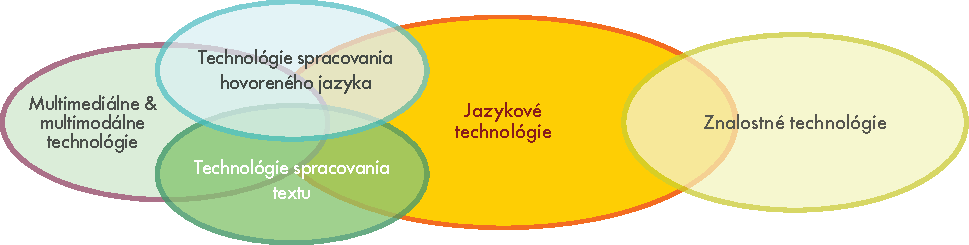
\includegraphics[width=\textwidth]{../_media/slovak/language_technologies}
  \caption{Záber jazykových technológií}
  \label{fig:ltincontextsk}
  \colorrule{grey3}{\textwidth}{1.5pt}
\end{figure*}

\subsection{Architektúra aplikácií}
Typické softvérové aplikácie na spracovanie jazyka sa
skladajú z~niekoľkých zložiek, ktoré odrážajú rôzne aspekty
jazyka a~úlohu, ktorú plnia. Obrázok~\ref{fig:textprocessingarch_sk}
zobrazuje veľmi zjednodušenú architektúru, ktorú možno nájsť
v~systéme na spracovanie textu. Prvé tri moduly sa zaoberajú
štruktúrou a~významom textového vstupu:

\begin{figure*}[hb]
  \colorrule{grey3}{\textwidth}{1.5pt}
  \center
  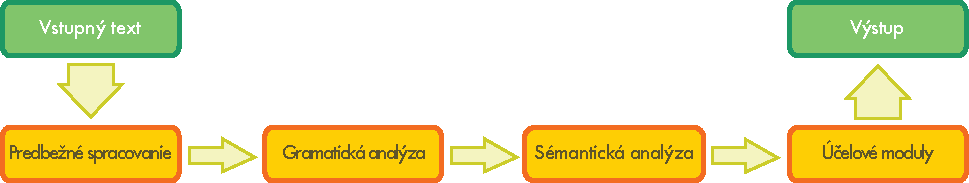
\includegraphics[width=\textwidth]{../_media/slovak/text_processing_app_architecture}
  \caption{Typická architektúra aplikácie na spracovanie textu}
  \label{fig:textprocessingarch_sk}
  \colorrule{grey3}{\textwidth}{1.5pt}
\end{figure*}

\begin{itemize}
\item Predbežné spracovanie: vyčistenie dát, odstránenie formátovania, detekcia vstupného jazyka, detekcia chýbajúcej diakritiky atď.
\item Gramatická analýza: hľadanie slovesa a~jeho prislúchajúceho predmetu alebo zvratného zámena atď.; zistenie vetnej štruktúry.
\item Sémantická analýza: odstránenie viacznačnosti (Ktorý význam slova \emph{mier} je správny v~danom kontexte?), vyriešenie anafory a~odkazujúcich výrazov ako \emph{on}, \emph{to auto} atď.; prezentácia významu vety v~strojovo čitateľnej forme.	
\end{itemize}

Moduly na špecifické úlohy potom vykonávajú rôzne operácie, ako je
automatická sumarizácia vstupného textu, databázové hľadania
a~mnoho ďalších. Ďalej ukážeme základné aplikačné oblasti
a~zdôrazníme ich základné moduly. Opäť pripomíname,
že architektúry aplikácií sú veľmi zjednodušené a~idealizované
pre vyjadrenie komplexnosti aplikácií jazykových technológií
všeobecne zrozumiteľným spôsobom.

Po predstavení základných aplikačných oblastí poskytneme stručný prehľad
situácie jazykových technológií v~oblasti výskumu a~vzdelávania, pričom na
záver uvedieme prehľad minulých a~prebiehajúcich výskumných programov. Na konci
tejto časti budeme prezentovať odborný odhad situácie oblasti základných
nástrojov a~zdrojov jazykových technológií z~viacerých hľadísk, napríklad z
hľadiska dostupnosti, zrelosti alebo kvality. Situácia jazykových technológií
pre slovenčinu je zobrazená v tabuľke na obrázku ~\ref{fig:lrlttable_sk} na konci tejto
kapitoly (s.~\pageref{fig:lrlttable_sk}). Tabuľka poskytuje prehľad všetkých
nástrojov a zdrojov, ktoré sú v texte zvýraznené tučným písmom. Jazykové
technológie pre slovenčinu sú porovnané s inými jazykmi, ktoré sú taktiež
súčasťou tejto série. 

\subsection{Základné aplikačné oblasti}
\subsubsection{Kontrola pravopisu}
Každý, kto používa kancelársky balík, ako napríklad LibreOffice, už pravdepodobne narazil na funkciu Kontrola pravopisu a~gramatiky, ktorá poukazuje na pravopisné chyby a~navrhuje ich opravu. 40 rokov po tom, čo Ralph Gorin uviedol prvý program na kontrolu pravopisu, sa tieto programy jazyka stali oveľa sofistikovanejšími a~už nepracujú len na princípe porovnávania zoznamu vybraných slov s~pravopisným slovníkom. Oproti jazykovo závislým algoritmom na zvládnutie morfológie (napr. tvorenie plurálu) existujú aj algoritmy schopné rozpoznať syntaktické chyby, typu chýbajúce sloveso alebo sloveso nezhodné s~podmetom v~osobe a~čísle, ako to môžeme pozorovať napríklad aj vo vete ‘She *write a~letter.’ („Ona písať list.“). Najdostupnejšie funkcie kontroly pravopisu (vrátane uplatnených v~balíku LibreOffice) však v~nasledujúcej prvej strofe básne Jerrolda H. Zara založenej na homofónii nenájdu žiadnu chybu (1992)\cite{f22}:

\begin{figure*}[htb]
  \colorrule{grey3}{\textwidth}{1.5pt}
  \center
  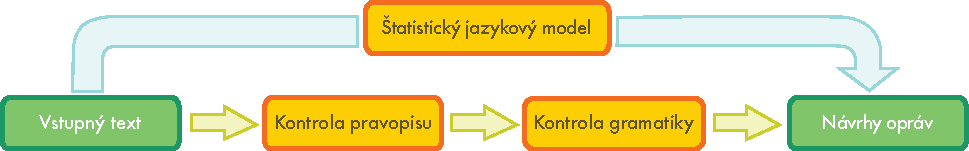
\includegraphics[width=\textwidth]{../_media/slovak/language_checking}
  \caption{Kontrola pravopisu a gramatiky (štatistická; na báze pravidiel)}
  \label{fig:langcheckingaarch_sk}
  \colorrule{grey3}{\textwidth}{1.5pt}
\end{figure*}

\begin{verse}
\emph{%
Eye have a~spelling chequer\\
It came with my Pea Sea.\\
It plane lee marks four my revue\\
Miss Steaks I~can knot sea.
}
\end{verse}

Na spracovanie tohto typu chýb je v~mnohých prípadoch potrebná analýza daného \underbar{kontextu}, ktorá je napríklad potrebná aj na rozhodnutie, či sa má isté slovo písať s~„y“ alebo s~„i“, ako napríklad v~prísloví:

\begin{verse}
\emph{%
Kto chce psa biť, palicu si nájde.\\
\smallskip
Kto chce psom byť, pána si nájde.
}
\end{verse}

Takýto postup si vyžaduje buď formuláciu gramatických
pravidiel špecifických pre daný jazyk, čo zároveň predpokladá
vysoký stupeň expertízy a~manuálnej práce, alebo využitie
takzvaného štatistického \underbar{jazykového modelu}. Takéto
modely prepočítavajú možnosť výskytu istého slova v~danom kontexte
(tzn. s~predchádzajúcimi a~nasledujúcimi slovami). Napríklad,
\emph{chce psom byť} je oveľa pravdepodobnejší sled slov ako
\emph{chce psom biť} a~naopak, \emph{chce psa biť} je oveľa
pravdepodobnejšia vetná konštrukcia než \emph{chce psa byť}
(napriek tomu by sme nepochybne dokázali vymyslieť kontexty,
v~ktorých sú gramaticky správne všetky štyri uvedené fragmenty).
Štatistický jazykový model môže byť automaticky derivovaný
využívaním veľkého množstva (korektných) jazykových dát (t.~j.
\underbar{korpusu}). Tieto prístupy však boli vyvinuté a~hodnotené
len na anglických jazykových dátach a~nedajú sa automaticky priamo
aplikovať na slovenčinu s~jej nestálym slovosledom a~bohatou flexiou.

Používanie funkcie Kontrola pravopisu a~gramatiky nie je obmedzené
len na nástroje spracovania textu, ale využíva sa aj
v~autorských systémoch. Spolu s~rastúcim počtom technických
produktov sa za posledné obdobie rapídne zvýšil aj počet technickej
dokumentácie. Strach spoločností zo sťažností zákazníkov
a~z~nárokov na náhradu škody, ktorá bola zapríčinená nesprávnymi
alebo nesprávne pochopenými inštrukciami, spôsobil, že sa
spoločnosti začali viac sústreďovať na kvalitu technickej
dokumentácie a~zároveň na medzinárodný trh. Pokroky
v~spracovávaní prirodzeného jazyka vedú k~rozvoju autorského
podporného softvéru, ktorý slúži zostavovateľovi technickej
dokumentácie na využívanie slovnej zásoby a~vetných štruktúr
v~súlade s~istými pravidlami a terminologickými
obmedzeniami.

%\begin{figure*}[htb]
%  \colorrule{grey3}{\textwidth}{1.5pt}
%  \center
%  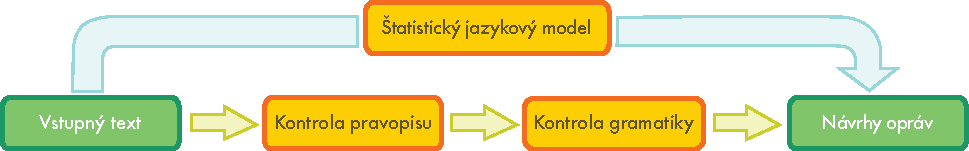
\includegraphics[width=\textwidth]{../_media/slovak/language_checking}
%  \caption{Kontrola pravopisu a gramatiky (štatistická; na báze pravidiel)}
%  \label{fig:langcheckingaarch_sk}
%  \colorrule{grey3}{\textwidth}{1.5pt}
%\end{figure*}

\boxtext{Funkcie kontroly pravopisu a~gramatiky pre slovenský jazyk
sú väčšinou založené na slovníku základných slovných tvarov
(lem) a súbore pravidiel na odvodenie ostatných tvarov}

Existujúce zariadenia kontroly pravopisu a~gramatiky pre slovenský
jazyk sú väčšinou založené na slovníku základných slovných
tvarov (lem) skombinovanom so súborom morfologických pravidiel, ktorý
umožňuje analýzu alebo generovanie všetkých (správnych) slovných
tvarov. Hoci sa zdá tento jednoduchý uspokojivý, má dve
zásadné nevýhody. Prvou nevýhodou je nesprávne určenie zdanlivo
správnych slovných tvarov v~dôsledku nesprávneho kontextu. Druhou
nevýhodou je neschopnosť rozlišovať skutočné pravopisné chyby od
správnych slovných tvarov, ktoré však nie sú obsiahnuté
v~slovníku. Takéto slová však budú vzhľadom na prirodzené
pribúdanie nových slov, vedeckých a~technických termínov
v~lexikóne existovať stále.

Okrem kontroly pravopisu a~autorizovanej podpory je funkcia kontrola
pravopisu a~gramatiky takisto dôležitá v~oblasti výučby jazyka. Aplikácie na kontrolu gramatiky a pravopisu taktiež dokážu pri preklepoch navrhnúť správne slovo, napríklad Google frázou „Mali ste na mysli\dots“

\subsubsection{Vyhľadávanie na webe}
Vyhľadávanie na webe, intranete alebo v~digitálnych knižniciach je dnes pravdepodobne najpoužívanejšia, no zároveň najmenej vyvinutá jazyková technológia. Google Vyhľadávač, ktorý vznikol v~roku 1998, sa v~súčasnosti využíva na vyhľadávanie 80~\% všetkých vyhľadávacích dopytov po celom svete. V~roku 2006 sa sloveso \emph{googlovať}/\emph{googliť} len veľmi tesne nestihlo zaradiť do prvého zväzku nového \emph{Slovníka súčasného slovenského jazyka}, čo sa jeho autorom neustále vyčítalo. Od prvej verzie Google sa dlhšiu dobu výrazne nezmenilo ani rozhranie vyhľadávania, ani zobrazovanie získaných výsledkov. V~súčasnej verzii ponúka Google opravu pravopisu nesprávne napísaných hľadaných slov a~v~roku 2009 začal vo svojich algoritmoch pracovať aj so základnou sémantickou analýzou\cite{pc1}, čo môže zvýšiť presnosť vyhľadávania analyzovaním významu požadovaných výrazov v~kontexte. Úspech spoločnosti Google poukazuje na fakt, že s~veľkým množstvom dostupných dát a~s~efektívnymi technikami na zaraďovanie týchto dát môže prevažne štatisticky založený prístup viesť k~uspokojivým výsledkom.

\begin{figure*}[htb]
  \colorrule{grey3}{\textwidth}{1.5pt}
  \center
  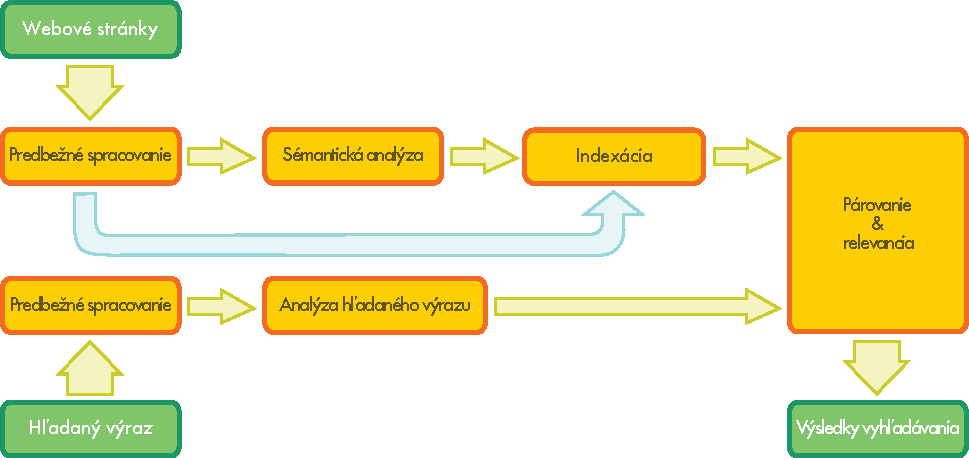
\includegraphics[width=\textwidth]{../_media/slovak/web_search_architecture}
  \caption{Architektúra vyhľadávania na webe}
  \label{fig:websearcharch_sk}
  \colorrule{grey3}{\textwidth}{1.5pt}
\end{figure*}

Pre sofistikovanejšie požadovanie informácií je však nevyhnutné integrovať hlbšie jazykové vedomosti. Experimenty vo výskumných laboratóriách s~používaním strojovo čitateľných \underbar{tezaurov} a~ontologických jazykových zdrojov ako WordNet ukázali, že je možné zvýšiť úspešnosť vyhľadávania umožnením vyhľadať stránku na základe synoným vyhľadávaných výrazov, napr. \emph{jadrová}, \emph{atómová} a~\emph{nukleárna energia} alebo dokonca aj nie veľmi súvisiacich pojmov. 

Budúca generácia vyhľadávačov musí zahrnúť oveľa sofistikovanejšie jazykové technológie. Ak hľadaná požiadavka nepozostáva zo zoznamu kľúčových slov, ale z~otázky alebo z~iného typu vety, získavanie relevantnej odpovede na danú požiadavku si vyžaduje syntaktickú a~sémantickú analýzu tejto vety, ako aj dostupnosť indexu, ktorý by počítal s~rýchlym získaním relevantných dokumentov. Predstavte si napríklad zadanú vstupnú požiadavku „Dajte mi zoznam spoločností, ktoré boli za posledných (niektorí ľudia by tu dokonca použili výraz „ostatných“ – ideálny vyhľadávací systém by si s~tým vedel poradiť) päť rokov odkúpené inými spoločnosťami“. Pre uspokojujúcu odpoveď je potrebná syntaktická {analýza} na určenie gramatických štruktúr vety a~stanovenie faktu, že zadávateľ hľadá spoločnosti, ktoré boli odkúpené, a~nie spoločnosti, ktoré ich odkúpili. Podobne musí byť spracovaný aj výraz \emph{posledných päť rokov}, aby sa zistilo, na ktoré roky sa výraz vzťahuje. 

\boxtext{Budúca generácia vyhľadávačov musí zahrnúť oveľa sofistikovanejšie jazykové technológie}

Pre úspešné vyhľadanie požadovanej informácie sa napokon musí spracovaná požiadavka porovnať s~obrovským množstvom neštruktúrovaných dát, v ktorých by sa vyhľadala aspoň časť požadovanej informácie. To sa často označuje termínom \underbar{získavanie informácií} a~zahŕňa vyhľadávanie a~posúdenie relevantných dokumentov. Navyše, ak chceme získať zoznam spoločností, potrebujeme extrahovať informácie, že určitý reťazec slov v~dokumente sa vzťahuje na názov spoločnosti. Tento druh informácie nám sprístupňujú takzvané \underbar{rozpoznávače pomenovaných entít}.

Ešte náročnejší je pokus spojiť zadávateľovu požiadavku
s~dokumentmi napísanými v~inom jazyku. Pre medzijazykové
získanie informácií musí byť požiadavka automaticky preložená
do všetkých možných východiskových jazykov a~získaná informácia
musí byť prenesená späť do cieľového jazyka. Rastúce percento
dát dostupných v~netextových formátoch zvyšuje dopyt po službách
umožňujúcich získavanie multimediálnych informácií,
tzn. vyhľadávanie obrázkov, zvukových a~obrazových dát. Pri
zvukových a~obrazových súboroch ide o~modul rozpoznávania
reči na konvertovanie rečového obsahu do textovej alebo fonetickej
podoby, ktorá by zodpovedala požiadavkám zadávateľa.

Na Slovensku existovali viaceré firmy, ktoré rozvíjali
technológie vyhľadávania, alebo sa takisto používali vyhľadávacie technológie
vyvinuté českými firmami. Prvý slovenský vyhľadávač, ktorý začal brať
do úvahy slovenskú morfológiu (vyvinutý na Matematicko-fyzikálnej
fakulte Karlovej univerzity v~Prahe), bol \emph{morfeo.sk}, prevádzkovaný
internetovým portálom \emph{centrum.sk}, ktorý začal poskytovať fulltextové
vyhľadávanie webových stránok s~doménou \emph{.sk} v~roku 2003. Na vyhľadávanie
ohýbaných slov využíval lematizáciu a~morfologickú anotáciu, aby tak
používateľovi poskytol relevantnejšie výsledky ako len tie, ktoré zahŕňali iba
základnú formu slov. Taktiež disponoval fuzzy vyhľadávaním. Do roku 2009 presiahol počet
indexovaných stránok 117 miliónov, pretože už vtedy Google zahrnul podporu
slovenskej morfológie, prevýšil počet indexovaných stránok a~\emph{centrum.sk}
prešlo na Google Vyhľadávanie.

V~tejto oblasti pracuje napríklad Forma, s.\,r.\,o.~\cite{f25}, ktorá na báze dát z~Jazykovedného ústavu Ľ. Štúra SAV vypracovala lingvistické moduly: jazykový korektor, rozdeľovač slov, lematizátor a~slovník synoným. Takisto má samostatné produkty na fulltextové vyhľadávanie v~slovenčine a~doteraz prevádzkuje vyhľadávanie v~starších verziách niektorých slovníkov.

Pozornosť pri rozvoji vyhľadávacích technológií sa kladie na poskytovanie doplnkov a~moderných vyhľadávačov pre záujmovo špecifické portály, pričom sa čo najviac využíva sémantika relevantná pre danú oblasť. Vzhľadom na vysoké nároky na výpočtový výkon sa takéto vyhľadávače využívajú len v~relatívne malých textových korpusoch. Časom spracovania a~tisícnásobným rozsahom ľahko prekoná bežný štatistický vyhľadávač, aký poskytuje napríklad Google. Tieto vyhľadávače majú vysoké nároky aj na modelovanie tematicky zameranej domény, čo znemožňuje používať tieto mechanizmy na webe. 

Tejto oblasti výskumu sa venuje hlavne Ústav informatiky SAV, kde sa v~roku 2006 začali venovať~oblasti spracovania písaného prirodzeného jazyka. V~tom čase sa inicioval aj vznik workshopov WIKT\cite{f26}, ktorých súčasťou je v~každom ročníku vydávanie niekoľkých článkov alebo celej sekcie venovanej spracovaniu slovenského jazyka. Výskum v~ÚI SAV v~spolupráci s~Univerzitou Pavla Jozefa Šafárika v~Košiciach sa od r. 2006 rozvíjal hlavne v~rámci projektu NAZOU\cite{f27}, kde sa tvorili nástroje na získanie, spracovanie, organizovanie a~prezentáciu informácií z~internetu. Konkrétnou aplikáciou boli pracovné ponuky, nástroje sa testovali aj na textoch slovenských pracovných ponúk. V~ÚI SAV bola vypracovaná analýza spracovania slovenčiny \cite{laclavik2007a} a~zároveň bol vyvinutý nástroj na extrakciu informácií Ontea\cite{f28} \cite{laclavik2007b,laclavik2009}, ktorý bol integrovaný s~nástrojmi na identifikáciu jazyka \cite{vojtek2006} a~nástrojom na lematizáciu \cite{krajci2007}.

Ontea pracuje na základe hľadania vzorov. Tieto vzory môžu byť
jednak jazykovo závislé vzory, ako napríklad použitie predložiek,
vetná skladba, ale aj jednoduchšie vzory typu použitie veľkých
písmen, skratiek, ako napríklad \emph{s.\,r.\,o.}, \emph{a.\,s.} na
hľadanie firiem, \emph{Sk}, \emph{SKK}, \emph{EUR}, \emph{EURO},
\emph{€} na hľadanie ceny, alebo skratiek slovenských krstných
mien na hľadanie osôb v~texte. Princíp je platný pre rôzne jazyky,
ale vzory sa musia tvoriť pre konkrétny jazyk, napríklad slovenčinu.
V~súčasnosti bol nástroj Ontea rozvíjaný na spracovanie e-mailovej
komunikácie. V~rámci projektu
AIIA\cite{f29} \cite{laclavik2010} bol
systém otestovaný na slovenských e-mailoch firmy Anasoft a~združenia
SANET. Ontea používa nielen vzory, ale aj slovníky urbanoným
(gazetteers), ako aj ich kombináciu na extrakciu a~identifikáciu
entít v~texte. Pri použití slovníkov (ale aj niektorých typov
hľadania) nastáva problém identifikácie entity, ak je v~inom ako
základnom tvare, preto~je vhodné použiť lematizátor. Keďže ide
hlavne o~názvoslovné entity ako ľudia, miesta, názvy produktov,
mená projektov alebo služieb, je ťažké ich lematizovať. Tieto
problémy sa zatiaľ nepodarilo uspokojivo vyriešiť, je však možné
riešiť ich novým spôsobom kombinácie slovníka, tokenizácie po
znakoch, lematizácie a~overenia entity v~slovníku.

Extrakcia entít pomocou vzorov bola použitá aj v~experimente na rozsiahlych dátach, keď sa spracúvali slovenské webové stránky s~cieľom extrakcie geografických dát (slovenských adries) a~následného vyhľadávania \cite{dlugolinsky2010}.

\subsubsection{Rečová technológia}
Rečová technológia tvorí základ na vytvorenie rozhrania, ktoré umožňuje používateľovi komunikovať so zariadeniami prostredníctvom hovoreného jazyka jednoduchšie než napríklad pomocou grafického displeja, klávesnice alebo myši. Dnes sa takéto hlasové používateľské rozhrania používajú na plne alebo čiastočne automatizované ponuky služieb poskytované spoločnosťami ich zákazníkom, zamestnancom alebo partnerom na telefóne. Obchodné činnosti, ktoré vo veľkej miere závisia od hlasových používateľských rozhraní, sú bankovníctvo, logistika, verejná doprava a~telekomunikácie. Iné využitia technológie rečovej interakcie sú rozhrania pre špeciálne zariadenia, napríklad navigačné systémy do  áut či~uplatnenie hovoreného jazyka ako alternatívy k~vstupno-výstupným modalitám grafických používateľských rozhraní, napríklad v~smartphonoch alebo tabletoch. 

\begin{figure*}[htb]
  \colorrule{grey3}{\textwidth}{1.5pt}
  \center
  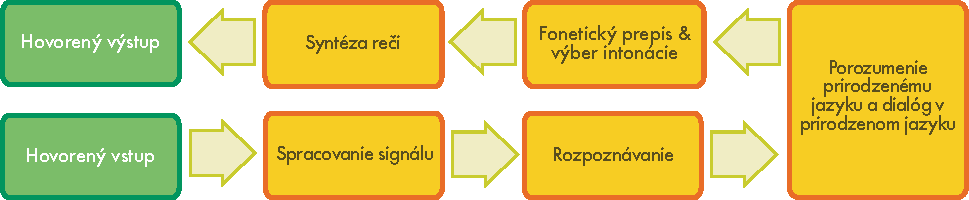
\includegraphics[width=\textwidth]{../_media/slovak/simple_speech-based_dialogue_architecture}
  \caption{Architektúra jednoduchého dialógového systému}
  \label{fig:dialoguearch_sk}
  \colorrule{grey3}{\textwidth}{1.5pt}
\end{figure*}

Vo svojej podstate pozostáva rečová interakcia zo štyroch rôznych technológií:

\begin{itemize}
\item Automatické rozpoznávanie reči zodpovedá za určenie, ktoré slová v~slede zvukov vypovedaných používateľom boli aktuálne hovorené.
\item Syntaktická analýza a~sémantická interpretácia sa zaoberajú analyzovaním syntaktickej štruktúry výpovede používateľa a~jej interpretáciou podľa účelu príslušného systému.
\item Dialógový manažment je potrebný pri určovaní opatrení, ktoré by sa mali podniknúť na strane systému, s~ktorým používateľ komunikuje, vzhľadom na vstup používateľa a~funkčnosť systému.
\item Rečová syntéza (Text-to-Speech, TTS) sa uplatňuje na transformovanie textovej výpovede do zvukovej formy, ktorá bude pre používateľa výstupom.
\end{itemize}

Jednou z~najväčších výziev je vytvoriť systém automatického
rozpoznávania reči, ktorý by dokázal čo najpresnejšie rozpoznať
používateľove slová. To si vyžaduje buď obmedzenie možných
výpovedí používateľa na limitovaný súbor kľúčových slov,
alebo manuálne vytvorenie jazykových modelov, ktoré by pokrývali
veľké množstvo prirodzených výpovedí v~jazyku používateľa.
Základnou požiadavkou pre dobrý výkon je takisto dobre natrénovaný
akustický model založený na obrovskom množstve zaznamenaných dát
rozlišujúcich prízvuk, vekovú skupinu, pohlavie atď. Kým prvá
možnosť vedie skôr k~strnulému a~nepružnému využívaniu
hlasového používateľského rozhrania a~pravdepodobne by ju
používatelia dobre neprijali, tvorenie, ladenie a~zlepšovanie
akustických a~jazykových modelov by zas výrazne zvýšilo náklady.
Hlasové používateľské rozhrania, ktoré využívajú jazykové
modely a dovoľujú na začiatku používateľovi flexibilne vyjadriť
svoju potrebu -- po vyzvaní napríklad frázou „Ako vám môžem
pomôcť“ -- vykazujú lepšiu možnosť automatizácie,
aj~lepšiu akceptáciu používateľmi, a teda majú výhodu oproti
než menej flexibilnému prístupu riadeného dialógu. Výnimku tvoria
tzv. embedded systémy,~ktoré vyžadujú na ovládanie relatívne málo
príkazov. V~takom prípade je použitie jazykových modelov
skôr nevýhodou a~aj dnes sa takéto systémy úspešne budujú
s~použitím gramatík.

Pre výstupné časti hlasového používateľského rozhrania inklinujú spoločnosti k~používaniu vopred nahraných výpovedí profesionálov – ideálne registrovaných hovoriacich. V~prípade statických výpovedí, ktorých obsah nezávisí od kontextu použitia alebo od osobných údajov daného používateľa, bude výsledkom vysoká spokojnosť používateľa. Čím dynamickejší bude obsah výpovede, tým väčšie problémy môže mať používateľ s~nejasnou prozódiou vyplývajúcou z~reťazenia jednotlivých zvukových segmentov. Dnešné systémy na syntézu reči sa vzhľadom na optimalizovateľnú prozodickú prirodzenosť dynamických výpovedí javia ako lepšie. 

Trh technológií rečovej interakcie prešiel počas poslednej dekády silnou štandardizáciou rozhraní medzi odlišnými technologickými komponentmi, ako aj štandardmi na tvorenie daných softvérových artefaktov pre danú aplikáciu. Za posledných desať rokov takisto prebieha silná konsolidácia trhu, hlavne v~oblasti automatického rozpoznávania reči a~syntézy reči. Národné trhy krajín G20, tzn.~ekonomicky silných krajín so značnou populáciou, sú celosvetovo ovládané niekoľkými veľkými súpermi, pričom Nuance, Google a~Microsoft patria dnes medzi najvýznamnejšie.

Na Slovensku má rozpoznávanie reči dlhú históriu, ale vykonávalo sa len na pôde univerzít a~vo vedeckých inštitúciách. Väčšina z~nich sa sústreďuje na základný výskum a~riešenia špecifických problémov rozpoznávania reči. Oddelenie analýzy a~syntézy reči Ústavu informatiky Slovenskej akadémie vied ako účastník projektu SpeechDat-E sa sústreďuje prevažne na akustické modely telefónnych systémov. S~rastúcim množstvom iných rečových nahrávok, ako napríklad parlamentné diskusie, sa ústav pomocou existujúcich nástrojov na rozpoznávanie reči snaží vytvoriť širšie použiteľné akustické modely pre  prepis diktovaného textu. Hlavný dôraz sa kladie na rozpoznávanie reči závislé od rečníka. Katedra elektroniky a~multimediálnych komunikácií Slovenskej Technickej univerzity v Bratislave sa sústreďuje hlavne na spracovanie rečového signálu v~podmienkach hluku (detekcia reči/hluku, extrahovanie atď.). Okrem mnohého iného vytvorila katedra aj početné malé systémy na rozpoznávanie reči, aby mohla porovnávať ich výkonnosť a~použiteľnosť na rozpoznávanie voľnej reči v~slovenskom jazyku. Na~Technickej univerzite v~Košiciach existujú viaceré katedry, ktoré sa sústreďujú na automatické rozpoznávanie reči. Katedra telekomunikácií Slovenskej technickej univerzity sa pôvodne zameriavala na základný výskum digitálneho spracovania rečového signálu, ktorý postupne svoj výskum zamerala na rozvoj rečových interaktívnych systémov.
\newline Katedra vytvorila v~spolupráci so Slovenskou akadémiou vied, Slovenskou technickou univerzitou a~Žilinskou univerzitou inteligentný komunikačný rečový systém, ktorý je prístupný verejnosti v~slovenskom jazyku a~demonštruje rečové interaktívne systémy pri telefonovaní. V~súčasnosti je na katedre jedným z~jej najpozoruhodnejších produktov v~oblasti jazykového modelovania systém na rozpoznávanie plynulej reči. Bázou jazykového modelu  je korpus pozostávajúci z~$2\cdot 10^9$ tokenov. 
\newline Druhé významné pracovné miesto na Technickej univerzite v~Košiciach je Katedra kybernetiky a~umelej inteligencie, kde bol pre slovenčinu vytvorený prvý rečový dialógový informačný systém a~fonetická abeceda SAMPA. Dnes na katedre zohrávajú aktivity týkajúce sa rozpoznávania reči okrajovú rolu. Katedra aplikovanej matematiky a~štatistiky na Fakulte matematiky, fyziky a~informatiky Univerzity Komenského v~Bratislave pracuje predovšetkým na rozpoznávaní reči prostredníctvom izolovaných slov detských hlasov. Výsledky boli aplikované vo vzdelávacom procese na verifikovanie textu čítaného deťmi. Zo zvukových dát zaznamenaných pre akustický modelový nácvik boli vytvorené len dve rečové databázy (\emph{Alica} a~\emph{Viktória}).  Hlavná inštitúcia na rozpoznávanie reči na Žilinskej univerzite je Katedra telekomunikácií a~multimédií. Jej tím sa zameriava predovšetkým na spracovanie digitálneho signálu pre rozpoznanie reči a~rozpoznávanie izolovaných slov pomocou použitia skrytých Markovovských modelov.

Úzka spolupráca medzi Katedrou elektroniky a~multimediálnych komunikácií TU v~Košiciach a~Oddelením analýzy a~syntézy reči Ústavu informatiky Slovenskej akadémie vied vyústila do prvých viditeľných úspechov rozvoja systému na rozpoznávanie plynulej reči. Výsledkom spolupráce je automatický systém prepisovania reči, ktorý možno využiť v~oblasti súdnictva.

Z~komerčných systémov na rozpoznávanie slovenského jazyka stojí za pozornosť produkt českej firmy Newton Technologies, ktorý možno považovať za prvý systém prepisovania v~slovenčine, ktorý je nezávislý od rečníka.

Odhliadnuc od súčasného stavu technológie môžeme konštatovať, že v~blízkej budúcnosti nastanú výrazné zmeny, ktoré budú okrem vplyvov telefónu, internetu a~e-mailových spojení podnietené hlavne rozšírením smartphonov ako novej platformy na manažovanie zákazníckych vzťahov. Tento trend ovplyvní aj využívanie technológií rečovej interakcie. Na jednej strane sa dopyt po hlasových používateľských rozhraniach na telefonickej báze postupom času zníži, na druhej strane používanie hovoreného jazyka ako užívateľsky komfortnej vstupnej modality pre smartphony výrazne získa na dôležitosti. Tento trend je podporovaný aj očividným zlepšením kvality rozpoznávania reči nezávisle od hovoriaceho, a~to pre potreby diktovania, ktoré sa už ponúkajú používateľom smartphonov ako centralizované služby. Ak posunieme outsourcing rozpoznávania reči do infraštruktúry aplikácií, využitie základných lingvistických technológií pre špecifické využitie pravdepodobne v~porovnaní so súčasnosťou získa na dôležitosti.  

\subsubsection{Strojový preklad}
S~myšlienkou využívať digitálne počítače na preklad
prirodzených jazykov prišiel v~roku 1946 A. D. Booth a~uchytila sa aj
vďaka značnej finančnej podpore tejto oblasti v~50. a~80. rokoch 20.
storočia. Napriek tomu sa \underbar{strojovému prekladu} nepodarilo
splniť očakávania, ktoré naň boli kladené už v~začiatočných
rokoch po jeho vzniku.

Strojový preklad jednoducho nahrádza slová jedného prirodzeného
jazyka slovami iného jazyka. To sa dá využiť v~oblastiach s~veľmi
obmedzeným, stereotypným jazykom, akým je napríklad jazyk predpovede
počasia. Pre dobrý preklad menej štandardizovaných textov však
treba pričleniť väčšie textové celky (frázy, vety alebo dokonca
celé pasáže) k~ich najbližším náprotivkom v~cieľovom jazyku.
Hlavný problém tkvie vo fakte, že ľudský jazyk je dvojznačný.
Jazyková dvojznačnosť prináša problémy na mnohých jazykových
úrovniach, napríklad \underbar{viacznačnosť slovných významov} na
lexikálnej rovine („Leopard“ môže znamenať zviera alebo
operačný systém) alebo pripojenie atribútov na syntaktickej rovine
ako v~príkladoch:

\begin{verse}
\emph{Otcovi priatelia neprišli, moji áno.}\\
\smallskip
\emph{Otcovi priatelia neprišli, mne áno.}
\end{verse}

Jeden z~možných prístupov k~problému sa zakladá na lingvistických
pravidlách. Pre preklad medzi blízko príbuznými jazykmi (ako však aj
už uvedených príkladoch) je prípustná aj metóda priameho prekladu.
Takéto systémy založené na pravidlách analyzujú vstupný text
a~vytvárajú „prostredníka“, symbolickú reprezentáciu, z~ktorej
sa generuje text cieľového jazyka. Úspech týchto metód veľmi
závisí od dostupnosti rozsiahlych lexikónov
s~morfologickými, syntaktickými a~sémantickými údajmi a~aj
s~veľkými súbormi \underbar{gramatických} pravidiel vypracovaných
skúsenými lingvistami. 

\begin{figure*}[htb]
  \colorrule{grey3}{\textwidth}{1.5pt}
  \center
  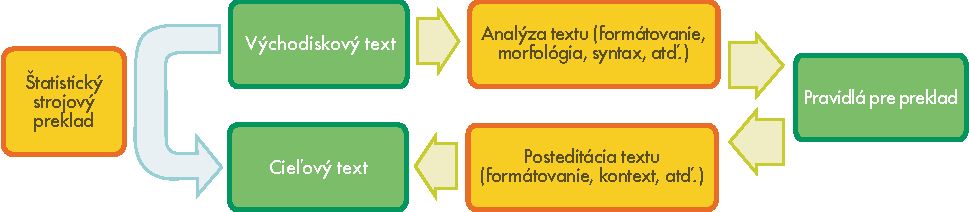
\includegraphics[width=\textwidth]{../_media/slovak/machine_translation}
  \caption{Strojový preklad (štatistický; založený na pravidlách)}
  \label{fig:mtarch_sk}
  \colorrule{grey3}{\textwidth}{1.5pt}
\end{figure*}

Koncom 80. rokov 20. storočia, teda v~čase, keď sa počítače
začali rozmáhať a~stali sa cenovo dostupnejšie, zvýšil sa záujem
o~štatistické modely pre strojový preklad. Parametre týchto
štatistických modelov sú odvodené z~analýzy bilingválneho
textového korpusu, akým je aj paralelný korpus Europarl,
ktorý obsahuje rokovania Európskeho parlamentu v~21 európskych
jazykoch. Ak dostane štatistický strojový preklad dostatok údajov,
funguje dostatočne dobre na to, aby odvodil približný význam
cudzieho jazyka v~texte. Na rozdiel od systémov riadených znalosťami
však štatistický (alebo dátami riadený) strojový preklad často
generuje gramaticky nesprávne výstupy. Na druhej strane však okrem
zníženej potreby ľudského úsilia na pravopisné písanie dokáže
strojový preklad riadený dátami pokryť také špecifiká jazyka,
akými sú napríklad idiomatické výrazy, ktoré zas chýbajú
v~systémoch riadených vedomosťami. 

Keďže sa silné a~slabé stránky strojového prekladu riadeného
vedomosťami a~strojového prekladu riadeného dátami navzájom
dopĺňajú, v~súčasnosti sa vedci usilujú kombinovaním oboch metód
uplatniť hybridné postupy. To je uskutočniteľné mnohými spôsobmi.
Jedným z~nich je možnosť použiť oba typy systémov a~nechať
rozhodnúť výberový modul o~najvhodnejšom výstupe pre každú vetu.
Pre dlhšie vety však nebude dokonalý žiadny výsledok. Lepším
riešením je preto skombinovanie najlepších častí každej vety
z~viacerých výstupov, čo však môže byť značne zložité, keďže
korešpondujúce časti rozličných alternatív nie sú vždy
zrozumiteľné a~musia byť nanovo usporiadané. 

V~90. rokoch 20. storočia bol navrhnutý prototyp strojového prekladu
medzi blízko príbuznou češtinou a~slovenčinou na Karlovej univerzite
v~Prahe.

TEOS Trenčín uviedol na trh prvý praktický mnohojazyčný softvér
strojového prekladu pre slovenský jazyk spolu s~ich PC slovníkovým
softvérom. Keďže však systém nepoužíval nijakú hlbšiu
lingvistickú analýzu a~jednoducho nahrádzal slová jedného jazyka
slovami druhého jazyka (zväčša obmedzené len na lemy), jeho
uplatnenie sa obmedzovalo len na jazyky, ktoré nedisponujú bohatým
morfologickým systémom, t.j. na angličtinu. Novšie verzie vedia
prekladať webové stránky za behu, čo je funkcia mimoriadne
užitočná pre anglicko-slovenské preklady (zároveň jediný
fungujúci smer prekladu).

\begin{figure*}[htbp]
  \centering
  \setlength{\tabcolsep}{0.17em}
  \small
  \begin{tabular}{>{\columncolor{corange1}}cccccccccccccccccccccccc}
    & \multicolumn{22}{>{\columncolor{corange1}}c}{Cieľový jazyk -- \textcolor{grey1}{Target language}}\\\addlinespace[{-.009cm}]
    \rowcolor{corange1}  & EN & BG & DE & CS & DA & EL & ES & ET & FI & FR & HU & IT & LT & LV & MT & NL & PL & PT & RO & SK & SL & SV\\
    EN & -- & \textcolor{blue}{40.5} & \textcolor{blue}{46.8} & \textcolor{green2}{52.6} & \textcolor{green2}{50.0} & \textcolor{blue}{41.0} & \textcolor{green2}{55.2} & \textcolor{purple}{34.8} & \textcolor{purple}{38.6} & \textcolor{green2}{50.1} & \textcolor{purple}{37.2} & \textcolor{green2}{50.4} & \textcolor{purple}{39.6} & \textcolor{blue}{43.4} & \textcolor{purple}{39.8} & \textcolor{green2}{52.3} & \textcolor{blue}{49.2} & \textcolor{green2}{55.0} & \textcolor{blue}{49.0} & \textcolor{blue}{44.7} & \textcolor{green2}{50.7} & \textcolor{green2}{52.0}\\
    BG & \textcolor{green}{61.3} & -- & \textcolor{purple}{38.7} & \textcolor{purple}{39.4} & \textcolor{purple}{39.6} & \textcolor{purple}{34.5} & \textcolor{blue}{46.9} & \textcolor{red3}{25.5} & \textcolor{red3}{26.7} & \textcolor{blue}{42.4} & \textcolor{red3}{22.0} & \textcolor{blue}{43.5} & \textcolor{red3}{29.3} & \textcolor{red3}{29.1} & \textcolor{red3}{25.9} & \textcolor{blue}{44.9} & \textcolor{purple}{35.1} & \textcolor{blue}{45.9} & \textcolor{purple}{36.8} & \textcolor{purple}{34.1} & \textcolor{purple}{34.1} & \textcolor{purple}{39.9}\\
    DE & \textcolor{green2}{53.6} & \textcolor{red3}{26.3} & -- & \textcolor{purple}{35.4} & \textcolor{blue}{43.1} & \textcolor{purple}{32.8} & \textcolor{blue}{47.1} & \textcolor{red3}{26.7} & \textcolor{red3}{29.5} & \textcolor{purple}{39.4} & \textcolor{red3}{27.6} & \textcolor{blue}{42.7} & \textcolor{red3}{27.6} & \textcolor{purple}{30.3} & \textcolor{red2}{19.8} & \textcolor{green2}{50.2} & \textcolor{purple}{30.2} & \textcolor{blue}{44.1} & \textcolor{purple}{30.7} & \textcolor{red3}{29.4} & \textcolor{purple}{31.4} & \textcolor{blue}{41.2}\\
    CS & \textcolor{green2}{58.4} & \textcolor{purple}{32.0} & \textcolor{blue}{42.6} & -- & \textcolor{blue}{43.6} & \textcolor{purple}{34.6} & \textcolor{blue}{48.9} & \textcolor{purple}{30.7} & \textcolor{purple}{30.5} & \textcolor{blue}{41.6} & \textcolor{red3}{27.4} & \textcolor{blue}{44.3} & \textcolor{purple}{34.5} & \textcolor{purple}{35.8} & \textcolor{red3}{26.3} & \textcolor{blue}{46.5} & \textcolor{purple}{39.2} & \textcolor{blue}{45.7} & \textcolor{purple}{36.5} & \textcolor{blue}{43.6} & \textcolor{blue}{41.3} & \textcolor{blue}{42.9}\\
    DA & \textcolor{green2}{57.6} & \textcolor{red3}{28.7} & \textcolor{blue}{44.1} & \textcolor{purple}{35.7} & -- & \textcolor{purple}{34.3} & \textcolor{blue}{47.5} & \textcolor{red3}{27.8} & \textcolor{purple}{31.6} & \textcolor{blue}{41.3} & \textcolor{red3}{24.2} & \textcolor{blue}{43.8} & \textcolor{red3}{29.7} & \textcolor{purple}{32.9} & \textcolor{red3}{21.1} & \textcolor{blue}{48.5} & \textcolor{purple}{34.3} & \textcolor{blue}{45.4} & \textcolor{purple}{33.9} & \textcolor{purple}{33.0} & \textcolor{purple}{36.2} & \textcolor{blue}{47.2}\\
    EL & \textcolor{green2}{59.5} & \textcolor{purple}{32.4} & \textcolor{blue}{43.1} & \textcolor{purple}{37.7} & \textcolor{blue}{44.5} & -- & \textcolor{green2}{54.0} & \textcolor{red3}{26.5} & \textcolor{red3}{29.0} & \textcolor{blue}{48.3} & \textcolor{red3}{23.7} & \textcolor{blue}{49.6} & \textcolor{red3}{29.0} & \textcolor{purple}{32.6} & \textcolor{red3}{23.8} & \textcolor{blue}{48.9} & \textcolor{purple}{34.2} & \textcolor{green2}{52.5} & \textcolor{purple}{37.2} & \textcolor{purple}{33.1} & \textcolor{purple}{36.3} & \textcolor{blue}{43.3}\\
    ES & \textcolor{green}{60.0} & \textcolor{purple}{31.1} & \textcolor{blue}{42.7} & \textcolor{purple}{37.5} & \textcolor{blue}{44.4} & \textcolor{purple}{39.4} & -- & \textcolor{red3}{25.4} & \textcolor{red3}{28.5} & \textcolor{green2}{51.3} & \textcolor{red3}{24.0} & \textcolor{green2}{51.7} & \textcolor{red3}{26.8} & \textcolor{purple}{30.5} & \textcolor{red3}{24.6} & \textcolor{blue}{48.8} & \textcolor{purple}{33.9} & \textcolor{green2}{57.3} & \textcolor{purple}{38.1} & \textcolor{purple}{31.7} & \textcolor{purple}{33.9} & \textcolor{blue}{43.7}\\
    ET & \textcolor{green2}{52.0} & \textcolor{red3}{24.6} & \textcolor{purple}{37.3} & \textcolor{purple}{35.2} & \textcolor{purple}{37.8} & \textcolor{red3}{28.2} & \textcolor{blue}{40.4} & -- & \textcolor{purple}{37.7} & \textcolor{purple}{33.4} & \textcolor{purple}{30.9} & \textcolor{purple}{37.0} & \textcolor{purple}{35.0} & \textcolor{purple}{36.9} & \textcolor{red3}{20.5} & \textcolor{blue}{41.3} & \textcolor{purple}{32.0} & \textcolor{purple}{37.8} & \textcolor{red3}{28.0} & \textcolor{purple}{30.6} & \textcolor{purple}{32.9} & \textcolor{purple}{37.3}\\
    FI & \textcolor{blue}{49.3} & \textcolor{red3}{23.2} & \textcolor{purple}{36.0} & \textcolor{purple}{32.0} & \textcolor{purple}{37.9} & \textcolor{red3}{27.2} & \textcolor{purple}{39.7} & \textcolor{purple}{34.9} & -- & \textcolor{red3}{29.5} & \textcolor{red3}{27.2} & \textcolor{purple}{36.6} & \textcolor{purple}{30.5} & \textcolor{purple}{32.5} & \textcolor{red2}{19.4} & \textcolor{blue}{40.6} & \textcolor{red3}{28.8} & \textcolor{purple}{37.5} & \textcolor{red3}{26.5} & \textcolor{red3}{27.3} & \textcolor{red3}{28.2} & \textcolor{purple}{37.6}\\
    FR & \textcolor{green}{64.0} & \textcolor{purple}{34.5} & \textcolor{blue}{45.1} & \textcolor{purple}{39.5} & \textcolor{blue}{47.4} & \textcolor{blue}{42.8} & \textcolor{green}{60.9} & \textcolor{red3}{26.7} & \textcolor{purple}{30.0} & -- & \textcolor{red3}{25.5} & \textcolor{green2}{56.1} & \textcolor{red3}{28.3} & \textcolor{purple}{31.9} & \textcolor{red3}{25.3} & \textcolor{green2}{51.6} & \textcolor{purple}{35.7} & \textcolor{green}{61.0} & \textcolor{blue}{43.8} & \textcolor{purple}{33.1} & \textcolor{purple}{35.6} & \textcolor{blue}{45.8}\\
    HU & \textcolor{blue}{48.0} & \textcolor{red3}{24.7} & \textcolor{purple}{34.3} & \textcolor{purple}{30.0} & \textcolor{purple}{33.0} & \textcolor{red3}{25.5} & \textcolor{purple}{34.1} & \textcolor{red3}{29.6} & \textcolor{red3}{29.4} & \textcolor{purple}{30.7} & -- & \textcolor{purple}{33.5} & \textcolor{red3}{29.6} & \textcolor{purple}{31.9} & \textcolor{red2}{18.1} & \textcolor{purple}{36.1} & \textcolor{red3}{29.8} & \textcolor{purple}{34.2} & \textcolor{red3}{25.7} & \textcolor{red3}{25.6} & \textcolor{red3}{28.2} & \textcolor{purple}{30.5}\\
    IT & \textcolor{green}{61.0} & \textcolor{purple}{32.1} & \textcolor{blue}{44.3} & \textcolor{purple}{38.9} & \textcolor{blue}{45.8} & \textcolor{blue}{40.6} & \textcolor{red3}{26.9} & \textcolor{red3}{25.0} & \textcolor{red3}{29.7} & \textcolor{green2}{52.7} & \textcolor{red3}{24.2} & -- & \textcolor{red3}{29.4} & \textcolor{purple}{32.6} & \textcolor{red3}{24.6} & \textcolor{green2}{50.5} & \textcolor{purple}{35.2} & \textcolor{green2}{56.5} & \textcolor{purple}{39.3} & \textcolor{purple}{32.5} & \textcolor{purple}{34.7} & \textcolor{blue}{44.3}\\
    LT & \textcolor{green2}{51.8} & \textcolor{red3}{27.6} & \textcolor{purple}{33.9} & \textcolor{purple}{37.0} & \textcolor{purple}{36.8} & \textcolor{red3}{26.5} & \textcolor{red3}{21.1} & \textcolor{purple}{34.2} & \textcolor{purple}{32.0} & \textcolor{purple}{34.4} & \textcolor{red3}{28.5} & \textcolor{purple}{36.8} & -- & \textcolor{blue}{40.1} & \textcolor{red3}{22.2} & \textcolor{purple}{38.1} & \textcolor{purple}{31.6} & \textcolor{purple}{31.6} & \textcolor{red3}{29.3} & \textcolor{purple}{31.8} & \textcolor{purple}{35.3} & \textcolor{purple}{35.3}\\
    LV & \textcolor{green2}{54.0} & \textcolor{red3}{29.1} & \textcolor{purple}{35.0} & \textcolor{purple}{37.8} & \textcolor{purple}{38.5} & \textcolor{red3}{29.7} & \textcolor{red2}{8.0} & \textcolor{purple}{34.2} & \textcolor{purple}{32.4} & \textcolor{purple}{35.6} & \textcolor{red3}{29.3} & \textcolor{purple}{38.9} & \textcolor{purple}{38.4} & -- & \textcolor{red3}{23.3} & \textcolor{blue}{41.5} & \textcolor{purple}{34.4} & \textcolor{purple}{39.6} & \textcolor{purple}{31.0} & \textcolor{purple}{33.3} & \textcolor{purple}{37.1} & \textcolor{purple}{38.0}\\
    MT & \textcolor{green}{72.1} & \textcolor{purple}{32.2} & \textcolor{purple}{37.2} & \textcolor{purple}{37.9} & \textcolor{purple}{38.9} & \textcolor{purple}{33.7} & \textcolor{blue}{48.7} & \textcolor{red3}{26.9} & \textcolor{red3}{25.8} & \textcolor{blue}{42.4} & \textcolor{red3}{22.4} & \textcolor{blue}{43.7} & \textcolor{purple}{30.2} & \textcolor{purple}{33.2} & -- & \textcolor{blue}{44.0} & \textcolor{purple}{37.1} & \textcolor{blue}{45.9} & \textcolor{purple}{38.9} & \textcolor{purple}{35.8} & \textcolor{blue}{40.0} & \textcolor{blue}{41.6}\\
    NL & \textcolor{green2}{56.9} & \textcolor{red3}{29.3} & \textcolor{blue}{46.9} & \textcolor{purple}{37.0} & \textcolor{blue}{45.4} & \textcolor{purple}{35.3} & \textcolor{blue}{49.7} & \textcolor{red3}{27.5} & \textcolor{red3}{29.8} & \textcolor{blue}{43.4} & \textcolor{red3}{25.3} & \textcolor{blue}{44.5} & \textcolor{red3}{28.6} & \textcolor{purple}{31.7} & \textcolor{red3}{22.0} & -- & \textcolor{purple}{32.0} & \textcolor{blue}{47.7} & \textcolor{purple}{33.0} & \textcolor{purple}{30.1} & \textcolor{purple}{34.6} & \textcolor{blue}{43.6}\\
    PL & \textcolor{green}{60.8} & \textcolor{purple}{31.5} & \textcolor{blue}{40.2} & \textcolor{blue}{44.2} & \textcolor{blue}{42.1} & \textcolor{purple}{34.2} & \textcolor{blue}{46.2} & \textcolor{red3}{29.2} & \textcolor{red3}{29.0} & \textcolor{blue}{40.0} & \textcolor{red3}{24.5} & \textcolor{blue}{43.2} & \textcolor{purple}{33.2} & \textcolor{purple}{35.6} & \textcolor{red3}{27.9} & \textcolor{blue}{44.8} & -- & \textcolor{blue}{44.1} & \textcolor{purple}{38.2} & \textcolor{purple}{38.2} & \textcolor{purple}{39.8} & \textcolor{blue}{42.1}\\
    PT & \textcolor{green}{60.7} & \textcolor{purple}{31.4} & \textcolor{blue}{42.9} & \textcolor{purple}{38.4} & \textcolor{blue}{42.8} & \textcolor{blue}{40.2} & \textcolor{green}{60.7} & \textcolor{red3}{26.4} & \textcolor{red3}{29.2} & \textcolor{green2}{53.2} & \textcolor{red3}{23.8} & \textcolor{green2}{52.8} & \textcolor{red3}{28.0} & \textcolor{purple}{31.5} & \textcolor{red3}{24.8} & \textcolor{blue}{49.3} & \textcolor{purple}{34.5} & -- & \textcolor{purple}{39.4} & \textcolor{purple}{32.1} & \textcolor{purple}{34.4} & \textcolor{blue}{43.9}\\
    RO & \textcolor{green}{60.8} & \textcolor{purple}{33.1} & \textcolor{purple}{38.5} & \textcolor{purple}{37.8} & \textcolor{blue}{40.3} & \textcolor{purple}{35.6} & \textcolor{green2}{50.4} & \textcolor{red3}{24.6} & \textcolor{red3}{26.2} & \textcolor{blue}{46.5} & \textcolor{red3}{25.0} & \textcolor{blue}{44.8} & \textcolor{red3}{28.4} & \textcolor{red3}{29.9} & \textcolor{red3}{28.7} & \textcolor{blue}{43.0} & \textcolor{purple}{35.8} & \textcolor{blue}{48.5} & -- & \textcolor{purple}{31.5} & \textcolor{purple}{35.1} & \textcolor{purple}{39.4}\\
    SK & \textcolor{green}{60.8} & \textcolor{purple}{32.6} & \textcolor{purple}{39.4} & \textcolor{blue}{48.1} & \textcolor{blue}{41.0} & \textcolor{purple}{33.3} & \textcolor{blue}{46.2} & \textcolor{red3}{29.8} & \textcolor{red3}{28.4} & \textcolor{purple}{39.4} & \textcolor{red3}{27.4} & \textcolor{blue}{41.8} & \textcolor{purple}{33.8} & \textcolor{purple}{36.7} & \textcolor{red3}{28.5} & \textcolor{blue}{44.4} & \textcolor{purple}{39.0} & \textcolor{blue}{43.3} & \textcolor{purple}{35.3} & -- & \textcolor{blue}{42.6} & \textcolor{blue}{41.8}\\
    SL & \textcolor{green}{61.0} & \textcolor{purple}{33.1} & \textcolor{purple}{37.9} & \textcolor{blue}{43.5} & \textcolor{blue}{42.6} & \textcolor{purple}{34.0} & \textcolor{blue}{47.0} & \textcolor{purple}{31.1} & \textcolor{red3}{28.8} & \textcolor{purple}{38.2} & \textcolor{red3}{25.7} & \textcolor{blue}{42.3} & \textcolor{purple}{34.6} & \textcolor{purple}{37.3} & \textcolor{purple}{30.0} & \textcolor{blue}{45.9} & \textcolor{purple}{38.2} & \textcolor{blue}{44.1} & \textcolor{purple}{35.8} & \textcolor{purple}{38.9} & -- & \textcolor{blue}{42.7}\\
    SV & \textcolor{green2}{58.5} & \textcolor{red3}{26.9} & \textcolor{blue}{41.0} & \textcolor{purple}{35.6} & \textcolor{blue}{46.6} & \textcolor{purple}{33.3} & \textcolor{blue}{46.6} & \textcolor{red3}{27.4} & \textcolor{purple}{30.9} & \textcolor{purple}{38.9} & \textcolor{red3}{22.7} & \textcolor{blue}{42.0} & \textcolor{red3}{28.2} & \textcolor{purple}{31.0} & \textcolor{red3}{23.7} & \textcolor{blue}{45.6} & \textcolor{purple}{32.2} & \textcolor{blue}{44.2} & \textcolor{purple}{32.7} & \textcolor{purple}{31.3} & \textcolor{purple}{33.5} & --\\
    \end{tabular}
  \caption{Strojový preklad medzi 22 jazykmi EU -- \textcolor{grey1}{Machine Translation between 22 EU-languages}\cite{euro1}}
  \label{fig:euromatrix_en}
\end{figure*}

Kvalita systémov strojového prekladu disponuje stále obrovským
potenciálom na zlepšenie. Súčasné výzvy spočívajú hlavne
v~adaptabilite jazykových zdrojov na danú doménu alebo
používateľskú oblasť a~v~ich integrácii do existujúceho
pracovného toku výrazových základní a~prekladových pamätí.
Väčšina súčasných systémov (nielen tých orientovaných na
slovenský jazyk) je orientovaná na angličtinu. Najvyššiu kvalitu
prekladu z/do angličtiny ponúka predovšetkým Google Translate. 

\boxtext{Kvalita systémov strojového prekladu disponuje stále obrovským potenciálom na zlepšenie}

Dostupnosť veľkého množstva bilingválnych textov je v~štatistickom
strojovom preklade skutočne kľúčová. Pre slovenčinu sa
v~súčasnosti korpus paralelných textov spolu s~mnohými inými
jazykmi len buduje. Najviac dát -- spolu milióny párov viet -- je
dostupných v~slovensko-českom a~slovensko-anglickom paralelnom
korpuse, ktorý sa zostavuje v~Jazykovednom ústave Ľ. Štúra. Obsah
korpusu tvorí prevažne beletria a~vety sú automaticky zarovnané.

Na obrázku~\ref{fig:euromatrix_en} (s.~\pageref{fig:euromatrix_en}) je tabuľka, ktorá bola vytvorená v rámci projektu Euromatrix+, znázorňuje presnosť prekladov medzi 22 jazykmi z 23 oficiálnych európskych jazykov (neporovnávala sa írčina). Výsledky sa hodnotili podľa BLUE skóre (čím viac bodov, tým lepší preklad) \cite{bleu1}. Za bežných podmienok dokáže človek získať približne 80 bodov.

\subsection{Ďalšie aplikačné oblasti}
Tvorba aplikácií jazykových technológií v~sebe zahŕňa množstvo čiastkových úloh, ktoré síce v~interakcii s~používateľom nevyjdú vždy na povrch, ale poskytujú rozličné funkcie skrytého systému. Koncipujú preto v~danej oblasti výskumu dôležité otázky, ktoré sa stali samostatnými akademickými subdisciplínami počítačovej lingvistiky.

\underbar{Zodpovedanie otázok} sa stalo aktívnou oblasťou výskumu,
pre ktorý boli vytvorené anotované korpusy a~ktorý odštartoval
vedecké súperenie. Idea spočíva v~posune od vyhľadávania pomocou
klávesnice (na ktoré prístroj odpovedá celým súborom potenciálne
relevantných dokumentov) k~variantu, v~ktorom používateľ kladie
konkrétnu otázku a~systém generuje jedinú odpoveď:

\begin{itemize}
	\item[] \textit{Otázka: Koľko rokov mal
Neil Armstrong, keď vystúpil na Mesiac?}
	\item[] \textit{Odpoveď: 38.}
\end{itemize}
Pokiaľ to súvisí
s~už spomínanou základnou oblasťou vyhľadávania na webe,
zodpovedanie otázok je predovšetkým zastrešujúcim výrazom
výskumných otázok typu: Aké \emph{druhy} otázok by sa mali
rozlišovať a~ako by sa malo s~nimi zaobchádzať, ako sa môže súbor
dokumentov, ktorý potenciálne obsahuje odpoveď, analyzovať
a~porovnávať (dávajú tieto dokumenty konfliktnú odpoveď?) a~ako
môže byť špecifická informácia – odpoveď – spoľahlivo
extrahovaná z~dokumentu bez neoprávneného ignorovania kontextu. 

To na druhej strane súvisí s~úlohou získavania informácií, s~oblasťou, ktorá sa tešila veľkej popularite a~vplyvu v~období „štatistického obratu“ v~počítačovej lingvistike v~raných 90. rokoch 20. storočia. Extrahovanie informácií sa sústreďuje na identifikáciu špecifických informácií v~špecifických triedach dokumentov; akými by mohli byť napríklad detekcia kľúčových hráčov prevzatia podnikov, ktorí sú uvedení v~novinových článkoch. Druhý variant, na ktorom sa pracovalo, sú správy o~teroristických útokoch, v~prípade ktorých problémom zostáva zmapovanie textu do šablóny špecifikujúcej páchateľa, cieľ, čas a~miesto útoku, ako aj jeho dôsledky. Doménovo špecifická náplň šablóny je ústrednou charakteristikou extrahovania informácií, ktorá je aj z~tohto dôvodu ďalším príkladom „zákulisnej“ technológie, ktorá predstavuje dobre ohraničenú oblasť výskumu, ale z~praktických dôvodov musí byť vsadená do vhodného aplikačného prostredia. 


JBOWL (Java knižnica \emph{Bag-Of-Words}) softvérová knižnica bola vyvinutá v~Centre pre informačné technológie (FEI-CIT) v~Košiciach na podporu NLP Text Mining aplikácií. JBOWL je modulárny systém umožňujúci spravovanie textových dokumentov. Poskytuje funkcie a~prostriedky podporujúce spracovanie textov prirodzeného jazyka (napr. tokenizáciu, morfologickú analýzu, lematizáciu, viacznačnosť, syntaktickú analýzu založenú na sieťach ATN, identifikáciu klasterov a~fráz, meranie závažnosti termínov a~ich označovanie), objavuje znalosti a~ťaží z~neštruktúrovaných textových dokumentov. Okrem iného systém implementuje viaceré algoritmy kontrolovaného a~nekontrolovaného strojového učenia s~nastaviteľnými vstupnými parametrami a~metódami na hodnotenie kvality modelov Text Miningu.

\boxtext{V Centre pre informačné technológie v Košiciach bola vyvinutá softvérová knižnica, ktorá spravuje textové dokumenty}

Dve hraničné oblasti, ktoré niekedy hrajú rolu samostatnej aplikácie a~inokedy rolu podporného, skrytého komponentu, sú sumarizovanie a~generovanie textu. Sumarizovanie zjavne súvisí s~úlohou skracovania textu a~ponúka sa napríklad aj ako funkcia MS Wordu. Pracuje prevažne na základe štatistických metód, pričom najprv identifikuje „dôležité“ slová v~texte (napríklad slová, ktoré sú v~tomto texte vysoko frekventované, ale výrazne menej používané v~bežnom jazyku), a~následne určuje tie vety, ktoré obsahujú veľa „dôležitých“ slov. Tieto vety sú v~dokumente vyznačené alebo sú z~neho extrahované a~použité na tvorbu sumáru. V~tomto variante, ktorý je doteraz najpoužívanejší, sa sumarizovanie rovná extrahovaniu viet: text je redukovaný na podskupinu jeho viet. Všetky komerčné sumarizéry využívajú práve tento nápad. Alternatívny postup, ktorému sa venuje len časť výskumu, spočíva v~aktuálnej syntéze \emph{nových} viet, t.~j. buduje súhrn viet, ktoré sa nemusia ukázať v~takejto forme vo východiskovom texte. Takýto postup si však vyžaduje určité hlbšie porozumenie textu a~je oveľa menej priamočiary. Textový generátor ako celok vo väčšine prípadov nie je samostatnou aplikáciou, ale je včlenený do väčšieho softvérového prostredia, ako napríklad do klinického informačného systému, kde sa údaje o~pacientoch zhromažďujú, skladujú, spracúvajú, pričom generovanie správ je len jednou z~mnohých funkcií. 

\subsection{Jazykové technológie vo vzdelávaní}
Jazykové technológie predstavujú vysoko interdisciplinárnu oblasť, ktorá si okrem iného vyžaduje expertízy lingvistov, vedcov výpočtovej techniky, matematikov, filozofov, psycholingvistov a~neurológov. Jazykové technológie si na slovenských fakultách stále hľadajú pevné miesto.

\boxtext{Pracovníci Ústavu informatiky SAV vedú kurz získavania informácií, grafových algoritmov na ich podporu a spracovania veľkého množstva dát}

Od roku 2007 viedli výskumníci z~Ústavu informatiky Slovenskej akadémie vied (Michal Laclavík a~Martin Šeleng) na Fakulte informačných technológií STU kurz získavania informácií, v ktorom sa zameriavali na problematiku získavania a~extrahovania informácií\cite{f30}, grafových algoritmov na ich podporu a~spracovania veľkého množstva dát. Študenti riešia v~tejto doméne rozličné projekty, pričom viacerí používajú slovenské zdroje, prípadne, niektorí riešia priamo problémy spracovania slovenského jazyka. Ako príklad uvádzame viaceré projekty zamerané na vytvorenie štatistického, slovníkovo orientovaného alebo algoritmického stemera založeného na projektoch Snowbal alebo Egothor, ako aj projekty zamerané na určovanie účinnosti a~štatistiky pri jednoduchých stemeroch, ktoré fungujú na princípe vynechania samohlások, diakritických znamienok, celých slovných zakončení atď. Takisto sem patria aj súbežne prebiehajúce projekty štatistických prekladov alebo tvorba automatického slovníka, ktorý prekladá medzi slovenčinou a~inými jazykmi (angličtinou, češtinou). Napokon sú to projekty využívajúce slovníky alebo frekvenčné jazykové slovníky pre aplikácie ako T9, extrahovanie pomenovaných entít s~použitím metód strojového učenia, knižnice ako OpenNLP, tvorba morfologického analyzátora, ako aj extrahovanie udalostí z~e-mailov alebo zo slovenských webových stránok a~pod.

Dodnes neexistuje žiadny pravidelný študijný program počítačovej lingvistiky.

\subsection{Štátne programy a iniciatívy}
Jazykové technológie a ich vývoj sa na Slovensku stále považujú za súčasť vedy a výskumu. Zaraďujú sa najmä do oblasti aplikovaného výskumu, a to v rámci lingvistiky (predovšetkým lexikografie) alebo informatiky. Kontakt s komerčnou sférou je nedostatočný až sporadický. V súčasnosti sa však začínajú jazykové technológie v značnej miere využívať v rôznych softvérových aplikáciách.

Prvé veľké projekty zamerané na jazykové technológie a zdroje na Slovensku boli osobitne schválené a financované vládou. Išlo o projekty \emph{Vybudovanie Národného korpusu slovenského jazyka a elektronizácia jazykovedného výskumu v rokoch 2002--2006} a \emph{Komplexné spracovanie slovenského jazyka a jeho elektronizácia na účely jazykovedného výskumu}. Oba projekty sa realizovali v Jazykovednom ústave Ľudovíta Štúra Slovenskej akadémie vied.

Projekt \emph{Vybudovanie Národného korpusu slovenského jazyka a elektronizácia jazykovedného výskumu v rokoch 2002–2006} bol schválený uznesením vlády č. 137/2002. Jeho cieľom bolo vybudovať reprezentatívny korpus slovenského jazyka, ktorý je nevyhnutným základom a materiálovým zdrojom pre všetky lingvistické výskumy a výskumy počítačového spracovania prirodzeného jazyka. Jazykový materiál korpusu je základnou bázou pri tvorbe veľkého lexikografického diela -- Slovníka súčasného slovenského jazyka. 

V rámci projektu sa vytvorilo oddelenie Slovenského národného korpusu, ktoré sa následne stalo vedúcim pracoviskom v oblasti spracovania prirodzeného jazyka na Slovensku. V rokoch 2007--2011 (druhá fáza) projekt pokračoval pod názvom \emph{Budovanie Slovenského národného korpusu a elektronizácia jazykovedného výskumu na Slovensku} na základe zmluvy a jeho spolufinancovaní medzi Ministerstvom školstva SR, Ministerstvom kultúry SR a SAV.

V rokoch 2003--2006 sa v rámci štátneho programu výskumu a vývoja Aktuálne otázky rozvoja spoločnosti zároveň realizovala úloha č. 2003SP200280307 \emph{Komplexné spracovanie slovenského jazyka a jeho elektronizácia na účely jazykovedného výskumu}. Vďaka riešeniu tejto úlohy sa mohli vyvíjať potrebné nástroje na počítačové spracovanie slovenského jazyka a rozširovať ďalšie zdroje: morfologická a syntaktická anotácia, elektronické lingvistické zdroje, terminologická databáza a pod. Výsledky tohto projektu sa využívajú a ďalej rozvíjajú v pokračujúcom projekte a našli si cestu aj do komerčnej sféry.

Ďalším významným projektom v spracovaní slovenského jazyka bol projekt \emph{APD
--  Automatický prepis diktátu pre Ministerstvo spravodlivosti Slovenskej
republiky} koordinovaný Oddelením analýzy a syntézy reči Ústavu informatiky
Slovenskej akadémie vied v spolupráci s Katedrou elektroniky a multimediálnych
komunikácií Technickej univerzity v Košiciach. Projekt sa realizoval v rokoch
2009--2011. Cieľom bolo vytvoriť kompletný systém na prepis hovoreného
slovenského jazyka, špeciálne v oblasti súdnictva. Projekt bol financovaný
Ministerstvom spravodlivosti Slovenskej republiky. V súčasnosti sa systém začína
využívať v pilotnej prevádzke na súdoch Slovenskej republiky.

Tieto projekty boli na Slovensku doteraz jedinou významnou iniciatívou v oblasti počítačového spracovania slovenčiny. Pripravili východisko pre hlbší výskum, ako aj rozmach komerčných projektov v tejto oblasti. Financovanie ďalšieho výskumu je však jednoznačne nevyhnuté. 


\subsection{Dostupnosť nástrojov a~zdrojov}
Na obrázku \ref{fig:lrlttable_sk} ponúkame sumarizáciu súčasného stavu jazykových technológií pre slovenčinu. Kritériá existujúcich nástrojov a~zdrojov v~rozmedzí 0 (veľmi nízky) až 6 (veľmi vysoký) navrhli poprední odborníci.

\begin{table*}[htb]
\centering

\begin{tabular}{>{\columncolor{orange1}}p{.33\linewidth}@{\hspace*{6mm}}c@{\hspace*{6mm}}c@{\hspace*{6mm}}c@{\hspace*{6mm}}c@{\hspace*{6mm}}c@{\hspace*{6mm}}c@{\hspace*{6mm}}c}
\rowcolor{orange1}
 \cellcolor{white}&
 \begin{sideways}\makecell[l]{Kvantita}\end{sideways} &
 \begin{sideways}\makecell[l]{\makecell[l]{Dostupnosť} }\end{sideways} &
 \begin{sideways}\makecell[l]{Kvalita}\end{sideways} &
 \begin{sideways}\makecell[l]{Pokrytie}\end{sideways} &
 \begin{sideways}\makecell[l]{Zrelosť}\end{sideways} &
 \begin{sideways}\makecell[l]{Udržateľnosť~~~}\end{sideways} &
 \begin{sideways}\makecell[l]{Adaptabilita}\end{sideways} \\ \addlinespace

\multicolumn{8}{>{\columncolor{orange2}}l}{\textcolor{black}{Jazyková technológia: Nástroje, technológie a aplikácie}} \\ \addlinespace

Rozpoznávanie reči	&3	&1	&2	&2	&3	&3	&2 \\ \addlinespace
Syntéza reči 		&3	&3	&3	&3	&3	&3	&3 \\ \addlinespace
Gramatická analýza 	&2	&2	&3	&2	&2	&3	&3 \\ \addlinespace
Sémantická analýza 	&1	&2	&1	&1	&1	&3	&3 \\ \addlinespace
Generovanie textu 		&1	&1	&1	&1	&0	&1	&1 \\ \addlinespace
Strojový preklad 	&2	&2	&2	&2	&2	&1	&2 \\ \addlinespace

\multicolumn{8}{>{\columncolor{orange2}}l}{\textcolor{black}{Jazykové zdroje: Zdroje, dáta a znalostné databázy}} \\ \addlinespace

Textové korpusy 		&2	&4	&4	&5	&4	&4	&4  \\ \addlinespace
Hovorené korpusy 		&3	&4	&2	&2	&3	&3	&3 \\ \addlinespace
Paralelné korpusy 	&2	&3	&2	&2	&2	&2	&3 \\ \addlinespace
Lexikálne zdroje 	&3	&2	&3	&4	&3	&4	&3 \\ \addlinespace
Gramatiky 		&2	&3	&3	&2	&1	&2	&1 \\
\end{tabular}
\caption{Stav podpory jazykových technológií v slovenčine}
\label{fig:lrlttable_sk}
\end{table*}

\begin{enumerate}
\item Kvantita: Existuje pre daný jazyk nejaký nástroj/zdroj? Čím viac nástrojov/zdrojov existuje, tým je hodnotenie vyššie.
\begin{itemize}
\item 0: neexistujú žiadne nástroje/zdroje
\item 6: mnoho nástrojov/zdrojov, veľká rôznorodosť
\end{itemize}
\item Dostupnosť: Sú nástroje/zdroje dostupné? - t.~j. sú Open Source voľne použiteľné na akejkoľvek platforme alebo sú dostupné len za vysokú cenu, resp. za obmedzených podmienok?
\begin{itemize}
\item 0: takmer všetky nástroje/zdroje sú dostupné len za vysokú cenu
\item 6: veľké množstvo nástrojov/zdro\-jov je voľne dostupných vďaka licenciám OpenSource, ako napr. Creative Commons, ktoré umožňujú opätovné použitie a~prispôsobenie potrebám používateľa (V prípade, že tam sú napr. dva rôzne zdroje, jeden z~nich úplne otvorený a~druhý úplne uzavretý, do tabuľky zadáme priemer (t.\,j.~3))
\end{itemize}
\item Kvalita: Do akej miery sa jednotlivé kritériá správania nástrojov a~ukazovatele kvality zdrojov približujú ku kvalite najlepších dostupných nástrojov, aplikácií či zdrojov? Sú tieto nástroje/zdroje aktuálne a~udržiavané?
\begin{itemize}
\item 0: amatérsky nástroj/zdroj
\item 6: kvalitný nástroj/zdroj, anotácie v~zdroji sa kvalitou rovnajú ručným anotáciám
\end{itemize}
\item Pokrytie: Do akej miery spĺňajú najlepšie dostupné nástroje príslušné kritériá pokrytia (štýlov, žánrov, druhov textov, jazykových javov, typov vstupov/výstupov, počtu jazykov podporovaných MT systémami atď.)? Do akej miery sú zdroje reprezentantmi daných jazykov, resp. subjazykov?
\begin{itemize}
\item 0: zdroj/nástroj určený na špecifické účely, osobité prípady, malé pokrytie, používa sa len vo veľmi špecifických, neobvyklých prípadoch
\item 6: zdroj so širokým pokrytím, robustný nástroj, široko uplatniteľný, veľké množstvo podporovaných jazykov
\end{itemize}
\item Vyspelosť: Môže sa nástroj/zdroj považovať za vyspelý, stabilný a~pripravený na trh? Dajú sa najlepšie dostupné nástroje/zdroje priamo použiť alebo sa musia upraviť? Je výkon takýchto technológií dostatočný a~použiteľný? Alebo sú to len prototypy, ktoré sú nevhodné pre produktívne systémy? Ukazovateľom vyspelosti môže byť prijatie nástrojov/zdrojov do komunity a~ich úspešné používanie v~systémoch jazykových technológií.
\begin{itemize}
\item 0: predbežný prototyp, amatérsky systém, overenie koncepcie
\item 6: okamžite integrovateľný/po\-u\-ži\-teľný prvok systému
\end{itemize}
\item Udržateľnosť: Ako sa dá nástroj/zdroj udržiavať, resp. integrovať do súčasných informačných systémov? Spĺňa nástroj/zdroj určitú úroveň udržateľnosti vzhľadom na dokumentáciu/manuály, vysvetlenie prípadov použitia, front‑endy, GUI atď.? Využíva daný nástroj štandardné/najspoľahlivejšie programovacie jazyky (napr. Java EE)? Existujú technické/výskumné normy, resp. kvázinormy? Ak áno, vyhovuje nástroj/zdroj týmto normám (dátové formáty a~pod.)?
\begin{itemize}
\item 0: súkromné zdroje, dátové formáty a~API ad hoc
\item 6: zdroje úplne vyhovujúce normám, kompletná dokumentácia
\end{itemize}
\item Adaptabilnosť: Do akej miery sa dajú najlepšie nástroje/zdroje adaptovať, resp. rozšíriť na nové úlohy/domény/žánre/typy textov/prí\-pa\-dy použitia atď.?
\begin{itemize}
\item 0: je prakticky nemožné adaptovať nástroj/zdroj na nové úlohy, dokonca ani s~použitím veľkého množstva zdrojov či človekohodín
\item 6: vysoká úroveň adaptabilnosti; nástroje/zdroje sa dajú veľmi jednoducho a~efektívne adaptovať
\end{itemize}
\end{enumerate}

\emph{Tabuľka sa dá zhrnúť do niekoľkých kľúčových bodov:}

\begin{itemize}
\item Na Slovensku existuje niekoľko špecializovaných kvalitných korpusov, ale dosiaľ tu nie je dostupný žiaden veľký, syntakticky anotovaný korpus.
\item Referenčným korpusom pre slovenčinu je Slovenský národný korpus. Kvôli licenčným obmedzeniam je však prístupné len jeho vyhľadávacie rozhranie.
\item Na druhej strane, korpus hovorených textov nepodlieha zákonu o~ochrane autorských práv a~je verejne dostupný. Jeho rozsah je však oproti rozsahu korpusu písaných textov nepatrný.
\item Mnohé zdroje sú neštandardizované, t.~j. aj keď existujú, nie sú udržiavané. Na štandardizáciu dát a~výmenu formátov je nevyhnutné spoločné úsilie a~iniciatíva.
\item Spracovať sémantiku je ťažšie ako spracovať syntax; spracovať textovú sémantiku je ťažšie než spracovať lexikálnu a~vetnú sémantiku.
\item Slovenčina má ontologický zdroj (zmapovaný na anglické ontologické zdroje), no jeho pokrytie je obmedzené.
\item V~zmysle reprezentácie vedomostí o~svete existujú štandardy pre sémantiku (RDF, OWL, atď.), ktoré sa však ťažko aplikujú na úlohy NLP.
\item Spracovanie písaného textu je rozvinutejšie ako spracovanie hovoreného textu (najmä rozpoznávania reči).
\item V~slovenčine chýbajú mnohé zdroje, ktoré sa v~iných jazykoch považujú za štandard; jazykový výskum NLP je na Slovensku veľmi slabo financovaný.
\item Niektoré výskumné a~vývojové aktivity pre slovenčinu sa realizujú v~Českej republike – ~na českých univerzitách alebo v~súkromnom sektore.
\item Výskum rozpoznávania reči pre slovenčinu prebieha na niekoľkých univerzitách a~výskumných pracoviskách, no množstvo voľne dostupných nástrojov a~dát je obmedzené.
\item Naopak, syntézu reči spracúvajú univerzity a~iné vedecké pracoviská v~oveľa menšom rozsahu.
\item V~oblasti syntézy reči sú dostupné OpenSource balíky a~niekoľko jednoduchých syntetizátorov reči, no syntéza reči s~prirodzenejšími hlasmi nie je dostupná.
\item Slovenské dialógové systémy sú veľmi málo rozšírené v~dôsledku nízkej dostupnosti kvalitných modulov rozpoznávania reči pre slovenčinu.
\end{itemize}

\subsection{Porovnanie jazykov}
Súčasný stav jazykových technológií je rozdielny v každej krajine. Na porovnanie situácie medzi jednotlivými jazykmi slúži nasledujúce ohodnotenie vzorových aplikácií v oblasti strojového prekladu a spracovania jazyka, textovej analýzy a zdrojov príslušného jazyka, ktoré sú nevyhnutné na tvorbu jazykových technológií. Tieto jazyky sa zoskupili na základe nasledujúcej päťbodovej škály:

% Cluster 1
\begin{figure*}[h!]
  \small
  \centering
  \begin{tabular}
  { 
  >{\columncolor{corange5}}p{.13\linewidth}@{\hspace{.040\linewidth}}
  >{\columncolor{corange4}}p{.13\linewidth}@{\hspace{.040\linewidth}}
  >{\columncolor{corange3}}p{.13\linewidth}@{\hspace{.040\linewidth}}
  >{\columncolor{corange2}}p{.13\linewidth}@{\hspace{.040\linewidth}}
  >{\columncolor{corange1}}p{.13\linewidth} 
  }
  \multicolumn{1}{>{\columncolor{white}}c@{\hspace{.040\linewidth}}}{\textbf{Vynikajúca
}} & 
  \multicolumn{1}{@{}>{\columncolor{white}}c@{\hspace{.040\linewidth}}}{\textbf{Veľmi dobrá}} &
  \multicolumn{1}{@{}>{\columncolor{white}}c@{\hspace{.040\linewidth}}}{\textbf{Dobrá}} &
  \multicolumn{1}{@{}>{\columncolor{white}}c@{\hspace{.040\linewidth}}}{\textbf{Čiastočná}} &
  \multicolumn{1}{@{}>{\columncolor{white}}c}{\textbf{Slabá/Žiadna}} \\ 
  \multicolumn{1}{>{\columncolor{white}}c@{\hspace{.040\linewidth}}}{\textbf{podpora
}} & 
  \multicolumn{1}{@{}>{\columncolor{white}}c@{\hspace{.040\linewidth}}}{\textbf{podpora
}} &
  \multicolumn{1}{@{}>{\columncolor{white}}c@{\hspace{.040\linewidth}}}{\textbf{podpora
}} &
  \multicolumn{1}{@{}>{\columncolor{white}}c@{\hspace{.040\linewidth}}}{\textbf{podpora
}} &
  \multicolumn{1}{@{}>{\columncolor{white}}c}{\textbf{podpora
}} \\ \addlinespace
& \vspace*{0.5mm}angličtina
& \vspace*{0.5mm}nemčina \newline   
taliančina \newline  
fínčina \newline 
francúzština \newline 
holandčina \newline 
portugalčina \newline 
španielčina \newline
čeština \newline 
& \vspace*{0.5mm}baskičtina \newline 
bulharčina \newline 
dánčina \newline 
estónčina \newline 
galícijčina \newline 
gréčtina \newline  
írčina \newline  
katalánčina \newline 
nórčina \newline 
poľština \newline 
švédčina \newline
srbčina \newline 
\textbf{slovenčina} \newline 
slovinčina \newline 
maďarčina  \newline
& \vspace*{0.5mm}islandčina \newline  
chorvátčina \newline 
lotyština \newline 
litovčina \newline 
maltčina \newline 
rumunčina\\
\end{tabular}
\label{fig:speech_cluster_sk}
\caption{Klastre jazykov pre spracovanie reči}
\end{figure*}

% Cluster 2
\begin{figure*}[h!]
  \small
  \centering
  \begin{tabular}
  { 
  >{\columncolor{corange5}}p{.13\linewidth}@{\hspace{.040\linewidth}}
  >{\columncolor{corange4}}p{.13\linewidth}@{\hspace{.040\linewidth}}
  >{\columncolor{corange3}}p{.13\linewidth}@{\hspace{.040\linewidth}}
  >{\columncolor{corange2}}p{.13\linewidth}@{\hspace{.040\linewidth}}
  >{\columncolor{corange1}}p{.13\linewidth} 
  }
  \multicolumn{1}{>{\columncolor{white}}c@{\hspace{.040\linewidth}}}{\textbf{Vynikajúca}} & 
  \multicolumn{1}{@{}>{\columncolor{white}}c@{\hspace{.040\linewidth}}}{\textbf{Veľmi dobrá}} &
  \multicolumn{1}{@{}>{\columncolor{white}}c@{\hspace{.040\linewidth}}}{\textbf{Dobrá}} &
  \multicolumn{1}{@{}>{\columncolor{white}}c@{\hspace{.040\linewidth}}}{\textbf{Čiastočná}} &
  \multicolumn{1}{@{}>{\columncolor{white}}c}{\textbf{Slabá/Žiadna}} \\ 
  \multicolumn{1}{>{\columncolor{white}}c@{\hspace{.040\linewidth}}}{\textbf{podpora}} & 
  \multicolumn{1}{@{}>{\columncolor{white}}c@{\hspace{.040\linewidth}}}{\textbf{podpora}} &
  \multicolumn{1}{@{}>{\columncolor{white}}c@{\hspace{.040\linewidth}}}{\textbf{podpora}} &
  \multicolumn{1}{@{}>{\columncolor{white}}c@{\hspace{.040\linewidth}}}{\textbf{podpora}} &
  \multicolumn{1}{@{}>{\columncolor{white}}c}{\textbf{podpora}} \\ \addlinespace
& \vspace*{0.5mm} angličtina 
& \vspace*{0.5mm} francúzština \newline 
španielčina
& \vspace*{0.5mm}nemčina \newline 
taliančina \newline 
katalánčina \newline
holandčina \newline 
poľština \newline 
rumunčina \newline 
maďarčina 
& \vspace*{0.5mm}baskičtina \newline 
bulharčina \newline 
dánčina \newline 
estónčina \newline 
fínčina \newline 
galícijčina \newline 
gréčtina \newline 
írčina \newline 
islandčina \newline 
chorvátčina \newline 
lotyština \newline 
litovčina \newline 
maltčina \newline 
nórčina \newline 
portugalčina \newline 
švédčina \newline 
srbčina \newline 
\textbf{slovenčina} \newline 
slovinčina \newline 
čeština \newline
\end{tabular}
\label{fig:mt_cluster_sk}
\caption{Klastre jazykov pre strojový preklad}
\end{figure*}

% Cluster 3
\begin{figure*}[h!]
  \small
  \centering
  \begin{tabular}
  { 
  >{\columncolor{corange5}}p{.13\linewidth}@{\hspace{.040\linewidth}}
  >{\columncolor{corange4}}p{.13\linewidth}@{\hspace{.040\linewidth}}
  >{\columncolor{corange3}}p{.13\linewidth}@{\hspace{.040\linewidth}}
  >{\columncolor{corange2}}p{.13\linewidth}@{\hspace{.040\linewidth}}
  >{\columncolor{corange1}}p{.13\linewidth} 
  }
  \multicolumn{1}{>{\columncolor{white}}c@{\hspace{.040\linewidth}}}{\textbf{Vynikajúca}} & 
  \multicolumn{1}{@{}>{\columncolor{white}}c@{\hspace{.040\linewidth}}}{\textbf{Veľmi dobrá}} &
  \multicolumn{1}{@{}>{\columncolor{white}}c@{\hspace{.040\linewidth}}}{\textbf{Dobrá}} &
  \multicolumn{1}{@{}>{\columncolor{white}}c@{\hspace{.040\linewidth}}}{\textbf{Čiastočná}} &
  \multicolumn{1}{@{}>{\columncolor{white}}c}{\textbf{Slabá/Žiadna}} \\ 
  \multicolumn{1}{>{\columncolor{white}}c@{\hspace{.040\linewidth}}}{\textbf{podpora}} & 
  \multicolumn{1}{@{}>{\columncolor{white}}c@{\hspace{.040\linewidth}}}{\textbf{podpora}} &
  \multicolumn{1}{@{}>{\columncolor{white}}c@{\hspace{.040\linewidth}}}{\textbf{podpora}} &
  \multicolumn{1}{@{}>{\columncolor{white}}c@{\hspace{.040\linewidth}}}{\textbf{podpora}} &
  \multicolumn{1}{@{}>{\columncolor{white}}c}{\textbf{podpora}} \\ \addlinespace
  & \vspace*{0.5mm}angličtina
& \vspace*{0.5mm}nemčina \newline 
  francúzština \newline 
  taliančina \newline 
  holandčina \newline 
  španielčina
& \vspace*{0.5mm}baskičtina \newline 
  bulharčina \newline 
  dánčina \newline 
  fínčina \newline 
  galícijčina \newline 
  gréčtina \newline 
  katalánčina \newline 
  nórčina \newline 
  poľština \newline 
  portugalčina \newline 
  rumunčina \newline 
  švédčina \newline 
  \textbf{slovenčina} \newline 
  slovinčina \newline 
  čeština \newline 
  maďarčina \newline 
& \vspace*{0.5mm}estónčina \newline 
  írčina \newline 
  islandčina \newline 
  chorvátčina \newline 
  lotyština \newline 
  litovčina \newline 
  maltčina \newline 
  srbčina \\
  \end{tabular}
\label{fig:text_cluster_sk}
\caption{Klastre jazykov pre textovú analýzu}
\end{figure*}

% Cluster 4
\begin{figure*}[h!]
  \small
  \centering
  \begin{tabular}
  { 
  >{\columncolor{corange5}}p{.13\linewidth}@{\hspace{.040\linewidth}}
  >{\columncolor{corange4}}p{.13\linewidth}@{\hspace{.040\linewidth}}
  >{\columncolor{corange3}}p{.13\linewidth}@{\hspace{.040\linewidth}}
  >{\columncolor{corange2}}p{.13\linewidth}@{\hspace{.040\linewidth}}
  >{\columncolor{corange1}}p{.13\linewidth} 
  }
  \multicolumn{1}{>{\columncolor{white}}c@{\hspace{.040\linewidth}}}{\textbf{Vynikajúca}} & 
  \multicolumn{1}{@{}>{\columncolor{white}}c@{\hspace{.040\linewidth}}}{\textbf{Veľmi dobrá}} &
  \multicolumn{1}{@{}>{\columncolor{white}}c@{\hspace{.040\linewidth}}}{\textbf{Dobrá}} &
  \multicolumn{1}{@{}>{\columncolor{white}}c@{\hspace{.040\linewidth}}}{\textbf{Čiastočná}} &
  \multicolumn{1}{@{}>{\columncolor{white}}c}{\textbf{Slabá/Žiadna}} \\ 
  \multicolumn{1}{>{\columncolor{white}}c@{\hspace{.040\linewidth}}}{\textbf{podpora}} & 
  \multicolumn{1}{@{}>{\columncolor{white}}c@{\hspace{.040\linewidth}}}{\textbf{podpora}} &
  \multicolumn{1}{@{}>{\columncolor{white}}c@{\hspace{.040\linewidth}}}{\textbf{podpora}} &
  \multicolumn{1}{@{}>{\columncolor{white}}c@{\hspace{.040\linewidth}}}{\textbf{podpora}} &
  \multicolumn{1}{@{}>{\columncolor{white}}c}{\textbf{podpora}} \\ \addlinespace
    
& \vspace*{0.5mm}angličtina
& \vspace*{0.5mm}nemčina \newline 
    francúzština \newline 
    holandčina \newline 
    švédčina \newline 
    čeština \newline 
    poľština \newline 
    maďarčina \newline
    taliančina \newline
    španielčina
& \vspace*{0.5mm} baskičtina \newline 
    bulharčina \newline 
    dánčina \newline 
    estónčina \newline 
    fínčina \newline 
    galícijčina \newline 
    gréčtina \newline 
    katalánčina \newline 
    chorvátčina \newline 
    nórčina \newline 
    portugalčina \newline 
    rumunčina \newline 
    srbčina \newline 
    \textbf{slovenčina} \newline 
    slovinčina \newline
&  \vspace*{0.5mm} írčina \newline 
    islandčina \newline 
    lotyština \newline 
    litovčina \newline 
    maltčina  \\
  \end{tabular}
  \caption{Klastre jazykov pre zdroje}
  \label{fig:resources_cluster_sk}
\end{figure*}

\begin{enumerate}
\item vynikajúca podpora
\item dobrá podpora
\item mierna podpora
\item čiastočná podpora
\item slabá alebo žiadna podpora
\end{enumerate}

Podpora jazykových technológií sa merala podľa nasledovných kritérií:

\begin{itemize}
\item Spracovanie reči: Kvalita existujúcich technológií na rozpoznávanie reči, kvalita existujúcich technológií rečovej syntézy, záber domén, počet a~veľkosť existujúcich hovorených korpusov, množstvo a~pestrosť dostupných na reči založených aplikácií
\item Strojový preklad: Kvalita existujúcich technológií strojového prekladu, počet pokrytých jazykových párov, pokrytie lingvistických fenoménov a~domén, kvalita a~veľkosť existujúcich paralelných korpusov, množstvo a~pestrosť dostupných aplikácií strojového prekladu
\item Textová analýza: Kvalita a~pokrytie existujúcich technológií textovej analýzy (morfológie, syntaxe, sémantiky), pokrytie lingvistických fenoménov a~domén, množstvo a~pestrosť dostupných aplikácií, kvalita a~veľkosť existujúcich (anotovaných) textových korpusov, kvalita a~pokrytie existujúcich lexikálnych zdrojov (napr. WordNet) a~gramatík
\item Zdroje: Kvalita a~veľkosť existujúcich textových korpusov, hovorených korpusov a~paralelných korpusov, kvalita a~pokrytie existujúcich lexikálnych zdrojov a~gramatík
\end{itemize} 

\subsection{Závery}
\emph{Touto sériou bielych kníh sme uskutočnili prvé kroky na stanovenie stupňa podpory jazykových technológií pre 30 európskych jazykov a na vysokej úrovni sme ponúkli porovnanie situácie medzi jednotlivými jazykmi. Po odhalení medzier, potrieb a nedostatkov môže Európska jazyková komunita a jej zainteresované strany realizovať rozsiahly výskum a rozvojový program s cieľom vybudovať s pomocou technológií v Európe skutočne multilingválnu komunikáciu.}

Biela kniha dokazuje, že na Slovensku existuje kvalitné prostredie pre
lingvistický výskum aj napriek tomu, že daný technologický priemysel sa tu
dostatočne nerozvinul. Slovenský výskum sa realizuje iba s malým počtom
dostupných technológií a zdrojov. Tento počet je nižší ako v prípade iných
jazykov ako sú čeština alebo poľština a podstatne nižší ako je to v prípade
hlavných jazykov EÚ (angličtiny, nemčiny alebo francúzštiny). Slovenské jazykové
technológie a zdroje majú navyše zjavne horšiu kvalitu.

Náš pohľad na technologickú podporu slovenského jazyka naozaj nemôže byť
optimistický. Na Slovensku máme rodiaci sa výskum v oblasti jazykových
technológií pre slovenčinu, a to najmä na univerzitách, vo vedeckých
pracoviskách, ako aj v malých a stredných podnikoch, ktoré sa zameriavajú na
základný výskum a riešenia špecifických problémov v oblasti jazykových
technológií. Rôzne inštitúcie zasvätili svoj výskum rozvoju jazykových
technológií, ako sú tvorba veľkých korpusov slovenčiny (písaných textov ale aj
hovoreného jazyka), morfologická analýza, strojový preklad, komplexné
rečové interaktívne systémy, rozpoznávanie reči a podobné.  Ich rozvoj je však
nutné ďalej rozvíjať a podporovať.

Ako uvádza táto správa, skôr ako bude možné urobiť nejaký posun v spracovávaní
slovenčiny, musia sa podniknúť okamžité kroky. Je jasné, že sa musí vynaložiť
väčšia snaha vytvoriť zdroje jazykových technológií pre slovenčinu a viesť
výskum, inováciu a rozvoj ako taký. Potreba veľkoobjemových dát a extrémna
komplikovanosť systémov jazykových technológií robí rozvoj novej infraštruktúry
veľmi dôležitým. Podporilo by to spoluprácu všetkých zainteresovaných strán.

Vo financovaní výskumu a rozvoja chýba kontinuita. Krátkodobo koordinované
programy sa striedajú s obdobiami nízkeho až zriedkavého financovania, pričom
je tu badateľný celkový nedostatok koordinácie programov v ďalších krajinách EÚ
a v samotnej Európskej komisii.

Slovenčine by spolu s ďalšími jazykmi pomohol väčší záujem o jazykové technológie a vytvorenie viacjazyčného programu pre európske krajiny a celý svet\cite{f32}.

\end{multicols}

\clearpage

\ssection[O META-NET-e]{O META-NET-e}
%\vspace*{-5mm}

\begin{multicols}{2}
  \textbf{META-NET} je sieť excelentnosti čiastočne financovaná
  z~fondov Európskej komisie. Sieť tvorí v~súčasnosti 54 výskumných
  centier z~33 krajín \cite{rehm2011}. META-NET buduje Multilingválnu
  európsku technologickú alianciu \textbf{META}, ktorá predstavuje
  narastajúcu komunitu profesionálov jazykových technológií
  a~organizácií v~Európe.

  META-NET podporuje technologické základy multilingválnej európskej
  informačnej spoločnosti tým, že:

\begin{itemize}
\item umožní komunikáciu a~spoluprácu v~rôznych jazykoch;
\item garantuje všetkým Európanom rovnaký prístup k~informáciám
  a~vedomostiam v~ľubovoľnom jazyku;
\item buduje a vylepšuje funkcie zosieťovaných informačných
  technológií.
\end{itemize}

Sieť podporuje Európu tým, že ju spája ako jediný digitálny trh a
informačný priestor. META-NET stimuluje a~podporuje rozvoj
viacjazyčných technológií všetkých európskych jazykov. Tieto
technológie využívajú automatický preklad, generujú obsah, spracúvajú
informácie, riadia vedomostný manažment a~i. Využívajú tiež intuitívne
jazykové rozhrania aplikovateľné na rozmanité technologické výdobytky
ako je domáca elektronika, stroje, autá alebo počítače či roboty.

Od 1.~februára 2010 v sebe META-NET zahŕňa tri nasledujúce okruhy
činností: META-VISION, META-SHARE a~META-RESEARCH.

\textbf{META-VISION} podporuje dynamickú a~vplyvnú komunitu
zainteresovaných strán, ktorú zjednocuje strategický výskumný program
(SRA; Strategic Research Agenda) pre oblasť európskych jazykových
technológií. Hlavným cieľom META-VISION je vytvoriť v~Európe ucelenú
a~súdržnú komunitu jazykových technológií cez zoskupenie rôznych
zainteresovaných strán. Súčasná séria Bielych kníh bola pripravovaná v
29 jazykoch. Spoločná technologická vízia sa vytvárala v troch
vizionárskych skupinách. Technologická rada META vznikla s cieľom
prediskutovať a pripraviť strategický výskumný program založený na
vízii vzájomnej spoluprácie celej komunity jazykových technológií.

\textbf{META-SHARE} vytvára možnosti na výmenu a~sprístupnenie
zdrojov. Sieť dátových úložísk bude obsahovať publikácie, súbory dát,
multimediálne súbory, výpočtové nástroje, služby a~aplikácie
usporiadané do štandardizovaných kategórií. Zdroje sa dajú jednoducho
vyhľadať. Sú to jednak bezplatné a~voľne prístupné materiály, ale aj
zdroje s~obmedzeným a~spoplatneným použitím.

\textbf{META-RESEARCH} spája príbuzné technologické oblasti. Táto
oblasť sa snaží využiť poznatky iných oblastí a~zužitkovať ich na
výskum jazykových technológií. Tento okruh sa obzvlášť zameriava na
špičkový výskum v oblasti strojového prekladu, zbierania dát, prípravy
dátových súborov a organizovania jazykových zdrojov na účel
hodnotenia; na zostavovanie inventára nástrojov a metód a
organizovanie seminárov či školení pre členov komunity.

\vfill
\textbf{\centerline{office@meta-net.eu -- http://www.meta-net.eu}}
\end{multicols}

\vfill

% End of original language part
% --------------------------------------------------------------------------

\makeatletter
\@ifundefined{theHsection}{
}
{
  \renewcommand*{\theHsection}{\thepart.\thesection}
}
\makeatother
\part*{\textcolor{white}{English}}
\setcounter{section}{0}
\setcounter{figure}{0}

\addtocontents{toc}{\protect\clearpage\protect}
\addtocontents{toc}{\protect\thispagestyle{empty}\protect}
\addtocontents{toc}{\protect\vspace*{4mm}\protect}
\addtocontents{toc}{\smallskip{\Large\textsf{\centerline{THE SLOVAK LANGUAGE IN THE DIGITAL AGE}}\par}}

\cleardoublepage

% --------------------------------------------------------------------------
% Start of english part
\selectlanguage{english}

% Chapter 1
\ssection[Executive Summary]{Executive Summary}
\begin{multicols}{2}
During the last 60 years, Europe has become a distinct political and economic structure, yet culturally and linguistically it is still very diverse. This means that from Portuguese to Polish and Italian to Icelandic, everyday communication between Europe’s citizens as well as communication in the spheres of business and politics is inevitably confronted with
 language barriers. The EU’s institutions spend about a billion euros a year on maintaining their policy of multilingualism, i.\,e., translating texts and interpreting spoken communication. Yet does this have to be such a burden? Modern language technology and linguistic research can make a significant contribution to pulling down these linguistic borders. When combined with intelligent devices and applications, language technology will in the future be able to help Europeans talk easily to each other and do business with each other even if they do not speak a common language. 

\boxtext{Language technology builds bridges}

One classic way of overcoming the language barrier is to learn foreign languages. Yet without technological support, mastering the 23 official languages of the member states of the European Union and some 60 other European languages is an insurmountable obstacle for the citizens of Europe and its economy, political debate, and scientific progress.   

The solution is to build key enabling technologies. These will offer European actors tremendous advantages, not only within the common European market but also in trade relations with third countries, especially emerging economies. To achieve this goal and preserve Europe’s cultural and linguistic diversity, it is necessary to first carry out a systematic analysis of the linguistic particularities of all European languages, and the current state of language technology support for them. Language technology solutions will eventually serve as a unique bridge between Europe’s languages. 

The automated translation and speech processing tools currently available on the market still fall short of this ambitious goal. The dominant actors in the field are primarily privately-owned for-profit enterprises based in Northern America. Already in the late 1970s, the EU realised the profound relevance of language technology as a driver of European unity, and began funding its first research projects, such as EUROTRA. At the same time, national projects were set up that generated valuable results but never led to concerted European action. In contrast to this highly selective funding effort, other multilingual societies such as India (22 official languages) and South Africa (11 official languages) have recently set up long-term national programmes for language research and technology development. 


The predominant actors in LT today rely on imprecise statistical approaches that do not make use of deeper linguistic methods and knowledge. For example, sentences are automatically translated by comparing a new sentence against thousands of sentences previously translated by humans. The quality of the output largely depends on the amount and quality of the available sample corpus. While the automatic translation of simple sentences in languages with sufficient amounts  of available text material can achieve useful results, such shallow statistical methods doomed to fail in the case of languages with a much smaller body of sample material or in the case of sentences with the complex structures.

\boxtext{Language technology as a key for the future}

The European Union has therefore decided to fund projects such as EuroMatrix and EuroMatrixPlus (since 2006) and iTranslate4 (since 2010) which carry out basic and applied research and generate resources for establishing high quality language technology solutions for all European languages. Analysing the deeper structural properties of languages is the only way forward if we want to build applications that perform well across the entire range of Europe’s languages.

European research in this area has already achieved a number of successes. For example, the translation services of the European Union now use MOSES open-source machine translation software that has been mainly developed through European research projects. The Verbmobil project, funded by the German Ministry of Education and Research, pushed Germany into the lead in the world of speech translation research for a time. Many of the research and development labs have since been closed down or moved elsewhere. Europe has tended to pursue isolated research activities with a less pervasive impact on the market.  

\boxtext{Language Technology helps unify Europe}

Drawing on the insights gained so far, it appears that today’s 'hybrid' language technology mixing deep processing with statistical methods will be able to bridge the gap between all European languages and beyond. As this series of white papers shows, there is a dramatic difference between Europe’s member states in terms of both the maturity of the research and in the state of readiness with respect to language solutions. 

META-NET’s long-term goal is to introduce high-quality language technology for all languages in order to achieve political and economic unity through cultural diversity. The technology will help tear down existing barriers and build bridges between Europe’s languages. This requires all stakeholders - in politics, research, business, and society - to unite their efforts for the future.

This white paper series complements other strategic actions taken by META-NET (see the appendix for an overview). Up-to-date information such as the current version of the META-NET vision paper\cite{Meta1} or the Strategic Research Agenda (SRA) can be found on the META-NET web site: \url{http://www.meta-net.eu}.

\end{multicols}

\clearpage

% Chapter 2
\ssection[Languages at Risk: a Challenge for Language Technology]{Languages at Risk: a Challenge for\newline Language Technology}

\begin{multicols}{2}
We are witnesses to a digital revolution that is dramatically impacting communication and society. Recent developments in digital information and communication technology are sometimes compared to Gutenberg’s invention of the printing press. What can this analogy tell us about the future of the European information society and our languages in particular?

\boxtext{The digital revolution is comparable to Gutenberg’s invention of the printing press.}

After Gutenberg’s invention, real breakthroughs in communication and knowledge exchange were accomplished by efforts such as Luther’s translation of the Bible into vernacular language. In subsequent centuries, cultural techniques have been developed to better handle language processing and knowledge exchange:

\begin{itemize}
\item the orthographic and grammatical standardisation of major languages enabled the rapid dissemination of new scientific and intellectual ideas;
\item the development of official languages made it possible for citizens to communicate within certain (often political) boundaries;
\item the teaching and translation of languages enabled exchanges across languages;
\item the creation of editorial and bibliographic guidelines assured the quality and availability of printed material;
\item the creation of different media like newspapers, radio, television, books, and other formats satisfied different communication needs. 
\end{itemize}

In the past twenty years, information technology has helped to automate and facilitate many of the processes:

\begin{itemize}
\item desktop publishing software has replaced typewriting and typesetting;
\item presentation software, such as OpenOffice/LibreOffice Impress or Microsoft PowerPoint has replaced overhead projector transparencies;
\item e-mail send and receive documents faster than a fax machine;
\item SIP telephony and Skype offers cheap Internet phone calls and hosts virtual meetings;
\item audio and video encoding formats make it easy to exchange multimedia content;
\item search engines provide keyword-based access to web pages;
\item online services like Google Translate produce quick, approximate translations;
\item social media platforms such as Facebook, Twitter, and Google+ facilitate communication, collaboration, and information sharing.
\end{itemize}

Although such tools and applications are helpful, they are not yet capable of supporting a sustainable, multilingual European society for all where information and goods can flow freely.

\subsection{Language Borders Hold back the European Information Society}
We cannot predict exactly what the future information society will look like. But there is a strong likelihood that the revolution in communication technology is bringing people speaking different languages together in new ways. This is putting pressure on individuals to learn new languages and especially on developers to create new technology applications to ensure mutual understanding and access to shareable knowledge. In a global economic and information space, more languages, speakers and content interact more quickly with new types of media. The current popularity of social media (Wikipedia, Facebook, Twitter, YouTube, Pokec, Google+) is only the tip of the iceberg.

\boxtext{The global economy and information space confronts us with different languages, speakers and content.}

Today, we can transmit gigabytes of text around the world in a few seconds before we recognise that it is in a language we do not understand. According to a recent report from the European Commission, 57\% of Internet users in Europe purchase goods and services in non-native languages. (English is the most common foreign language followed by French, German and Spanish.) 55\% of users read content in a foreign language while only 35\% use another language to write e-mails or post comments on the Web\cite{EC1}. A few years ago, English might have been the lingua franca of the Web—the vast majority of content on the Web was in English—but the situation has now drastically changed. The amount of online content in other European (as well as Asian and Middle Eastern) languages has exploded.

Surprisingly, this ubiquitous digital divide due to language borders has not gained much public attention; yet, it raises a very pressing question: Which European languages will thrive in the networked information and knowledge society, and which are doomed to disappear?

\subsection{Our Languages at Risk}
While the printing press helped step up the exchange of information in Europe, it also led to the extinction of many European languages. Regional and minority languages were rarely printed and languages such as Romani and Rusyn were mostly limited to oral forms of transmission, which in turn restricted their scope of use. Will the Internet have the same impact on our languages?

\boxtext{The variety of languages in Europe is one of its richest and most important cultural assets.}
 
Europe’s approximately 80 languages are one of its richest and most important cultural assets, and a vital part of its unique social model\cite{EC2}. While languages such as English and Spanish are likely to survive in the emerging digital marketplace, many European languages could become irrelevant in a networked society. This would weaken Europe’s global standing, and run counter to the strategic goal of ensuring equal participation for every European citizen regardless of language. According to a UNESCO report on multilingualism, languages are an essential medium for the enjoyment of fundamental rights, such as political expression, education and participation in society\cite{Unesco1}.
\vfill

\subsection{Language Technology is a Key Enabling Technology}
In the past, investment efforts in language preservation focused on language education and translation. According to one estimate, the European market for translation, interpretation, software localisation and website globalisation was €8.4 billion (short scale, i.\,e., $8.4\cdot 10^9$.) in 2008 and is expected to grow by 10\% per annum\cite{EC3}. Yet this figure covers just a small proportion of current and future needs in communicating between languages. The most compelling solution for ensuring the breadth and depth of language usage in Europe tomorrow is to use appropriate technology, just as we use technology to solve our transport, energy and disability needs among others.

Digital language technology (targeting all forms of written text and spoken discourse) helps people collaborate, conduct business, share knowledge and participate in social and political debate regardless of language barriers and computer skills. It often operates invisibly inside complex software systems to help us:

\begin{itemize}
\item find information with an Internet search engine;
\item check spelling and grammar in a word processor;
\item view product recommendations in an online shop;
\item hear the verbal instructions of a car navigation system;
\item translate web pages via an online service.
\end{itemize}

Language technology consists of a number of core applications that enable processes within a larger application framework. The purpose of the META-NET language white papers is to focus on how ready these core technologies are for each European language.

To maintain our position in the frontline of global innovation, Europe will need language technology adapted to all European languages that is robust, affordable and tightly integrated within key software environments. Without language technology, we will not be able to achieve a really effective interactive, multimedia and multilingual user experience in the immediate future. 

\subsection{Opportunities for Language Technology}
In the world of print, the technology breakthrough was the rapid
duplication of an image of a text (a page) using a suitably powered
printing press. Human beings had to do the hard work of looking up,
reading, translating, and summarizing knowledge. We had to wait until
Edison to record spoken language – and again his technology simply
made analogue copies.

Digital language technology can now automate the very processes of translation, content production, and knowledge management for all European languages. It can also empower intuitive language/speech-based interfaces for household electronics, machinery, vehicles, computers and robots. Real-world commercial and industrial applications are still in the early stages of development, yet R\&D achievements are creating a genuine window of opportunity. For example, machine translation is already reasonably accurate in specific domains, and experimental applications provide multilingual information and knowledge management as well as content production in many European languages. 

As with most technologies, the first language applications such as voice-based user interfaces and dialogue systems were developed for highly specialised domains, and often exhibit limited performance. But there are huge market opportunities in the education and entertainment industries for integrating language technologies into games, cultural heritage sites, edutainment packages, libraries, simulation environments and training programmes. Mobile information services, computer-assisted language learning software, e-learning environments, self-assessment tools and plagiarism detection software are just some of the application areas where language technology can play an important role. The popularity of social media applications like Twitter, Pokec or Facebook suggest a further need for sophisticated language technologies that can monitor posts, summarise discussions, suggest opinion trends, detect emotional responses, identify copyright infringements or track misuse.

\boxtext{Language technology helps overcome the ``disability'' of linguistic diversity}

Language technology represents a tremendous opportunity for the European Union. It can help address the complex issue of multilingualism in Europe – the fact that different languages coexist naturally in European businesses, organisations and schools. But citizens need to communicate across these language borders criss-crossing the European Common Market, and language technology can help overcome this final barrier while supporting the free and open use of individual languages. Looking even further forward, innovative European multilingual language technology will provide a benchmark for our global partners when they begin to enable their own multilingual communities. Language technology can be seen as a form of ‘assistive’ technology that helps overcome the ‘disability’ of linguistic diversity and make language communities more accessible to each other.

Finally, one active field of research is the use of language technology for rescue operations in disaster areas, where performance can be a matter of life and death: Future intelligent robots with cross-lingual language capabilities have the potential to save lives.

\subsection{Challenges Facing Language Technology}

Although language technology has made considerable progress in the last few years, the current pace of technological progress and product innovation is too slow. Widely-used technologies such as the spelling and grammar correctors in word processors are typically monolingual, and are only available for a handful of languages. Online machine translation services, although useful for quickly generating a reasonable approximation of a document’s contents, are fraught with difficulties when highly accurate and complete translations are required. Due to the complexity of human language, modelling our tongues in software and testing them in the real world is a long, costly business that requires sustained funding commitments. Europe must therefore maintain its pioneering role in facing the technology challenges of a multiple-language community by inventing new methods to accelerate development right across the map. These could include both computational advances and techniques such as crowdsourcing.

\boxtext{Technological progress needs to be accelerated.}

\subsection{Language Acquisition in Humans and Machines}
To illustrate how computers handle language and why it is difficult to program them to use it, let’s look briefly at the way humans acquire first and second languages, and then see how language technology systems work. 

Humans acquire language skills in two different ways. Babies acquire a language by listening to the real interactions between its parents, siblings and other family members. From the age of about two, children produce their first words and short phrases. This is only possible because humans have a genetic disposition to imitate and then rationalise what they hear. 

Learning a second language at an older age requires more effort, largely because the child is not immersed in a language community of native speakers. At school, foreign languages are usually acquired by learning grammatical structure, vocabulary and spelling using drills that describe linguistic knowledge in terms of abstract rules, tables and examples. Learning a foreign language gets harder with age.

\boxtext{Humans acquire language skills in two different ways: learning from examples and learning the underlying language rules.}

The two main types of language technology systems ‘acquire’ language capabilities in a similar manner. Statistical (or ‘data-driven’) approaches obtain linguistic knowledge from vast collections of concrete example texts. While it is sufficient to use text in a single language for training, e.\,g., a spell checker, parallel texts in two (or more) languages have to be available for training a machine translation system. The machine learning algorithm then “learns” patterns of how words, short phrases and complete sentences are translated. 

This statistical approach can require millions of sentences and performance quality increases with the amount of text analysed. This is one reason why search engine providers are eager to collect as much written material as possible. Spelling correction in word processors, and services such as Google Search and Google Translate all rely on statistical approaches. The great advantage of statistics is that the machine learns fast in continuous series of training cycles, even though quality can vary arbitrarily.

The second approach to language technology and machine translation in particular is to build rule-based systems. Experts in the fields of linguistics, computational linguistics and computer science first have to encode grammatical analyses (translation rules) and compile vocabulary lists (lexicons). This is very time consuming and labour intensive. Some of the leading rule-based machine translation systems have been under constant development for more than twenty years. The great advantage of rule-based systems is that the experts have more detailed control over the language processing. This makes it possible to systematically correct mistakes in the software and give detailed feedback to the user, especially when rule-based systems are used for language learning. But due to the high cost of this work, rule-based language technology has so far only been developed for major languages. 

As the strengths and weaknesses of statistical and rule-based systems tend to be complementary, current research focuses on hybrid approaches that combine the two methodologies. However, these approaches have so far been less successful in industrial applications than in the research lab. 

As we have seen in this chapter, many applications widely used in today’s information society rely heavily on language technology. Due to its multilingual community, this is particularly true of Europe’s economic and information space. Although language technology has made considerable progress in the last few years, there is still huge potential in improving the quality of language technology systems. In the following, we will describe the role of Slovak in European information society and assess the current state of language technology for the Slovak language. 

\end{multicols}

\clearpage

% Chapter 3
%FIXME structure
\ssection[Slovak in the European Information Society]{Slovak in the European Information Society}
\begin{multicols}{2}
\subsection{General Facts}
The Slovak Republic is a country in Central Europe neighbouring both Slavic (Czech Republic, Poland, Ukraine) and non-Slavic countries (Hungary, Austria). Its geographic location, mostly mountainous landscape and historical development created the considerably multi-ethnic and multicultural character of the country. It also caused a variety of Slovak dialects and the subsequent codification of (modern) standard Slovak as an over-regional communication mean by as late as 1843. Although part of the territory of Slovakia belonged to the historic Great Moravia, where Constantine and Methodius, invited from the Byzantine Empire in the 9\textsuperscript{th} century were spreading the Christian religion and education through Old Church Slavonic and the Glagolitic alphabet. Later development of Slovakia and the Slovak language was influenced by the Latin alphabet and Roman culture. Several influences subsequently occurred that left traces on the Slovak language as well.

The Slovak language– in the Indo-European family of languages, together with Polish, Czech, Lower and Upper Sorbian – belongs to the West branch of Slavic languages. Linguistic, historic, and archaeological sources prove that Slovak developed directly from Proto-Slavic. The Proto-Slavic basis of Slovak was formed in the area between the Carpathians, the Danube, and the Upper Moravia. The Slavonians, predecessors of the Slovaks, came to this area in the 6\textsuperscript{th} century from the south-east. The reconstructed language of the Great Moravian ethnic group, which was divided into dialects but formed a certain cultural form can be regarded as the basis of Slovak. The Slovak language went through fast development in the 10\textsuperscript{th} to 12\textsuperscript{th} centuries (jer vocalisation, disappearance of nasal vowels), and stabilised in the 13\textsuperscript{th} to 15\textsuperscript{th} centuries. In the 16\textsuperscript{th} to 18\textsuperscript{th} centuries, Czech was used as the cultural language in Slovakia, together with several types of cultural Slovak, such as cultural West Slovak, cultural Central Slovak and cultural East Slovak. By the end of the 18\textsuperscript{th} century, attempts at the formation of literary Slovak had started. At the end of the 18\textsuperscript{th} century, Anton Bernolák based his codification on cultural West Slovak, but failed to get wide recognition due to changed social and economic conditions. Ľudovít Štúr used Central Slovak as the basis and his idea took hold very soon, and with certain modifications (Martin Hattala, Michal Miloslav Hodža) lasts up to these days.

Slovak is the official language in the Slovak Republic. Since May 2004 it has also been one of the administrative languages of the European Union. Slovak is spoken by 4.5 million inhabitants of Slovakia, more than 1 million emigrants in the United States, and approx. 300 thousand people in the Czech Republic. Smaller language groups of Slovaks are situated in Hungary, Romania, Serbia, Croatia, Bulgaria, Poland, the United Kingdom, France, Germany, Belgium, Austria, Norway, Denmark, Finland, Sweden, Italy, Switzerland, the Netherlands, Cyprus, Russia, Ukraine, Kyrgyzstan, Israel, Canada, South Africa, Argentina, Brazil, Uruguay, Australia, New Zealand,  and other countries. Slovak language is ``esperanto'' of all the Slavic languages due to its most comprehensible character for other users of Slavic langugages.

\boxtext{Slovak language is ``esperanto'' of all the Slavic languages}

 Slovaks abroad pertain to different groups: they are descendants of indigenous
inhabitants of Slovakia, who moved to other areas of former Austro-Hungary;
descendants of later migrants from Slovakia, living overseas (emigration wave
from the late 19\textsuperscript{th} to the mid 20\textsuperscript{th}
century); political and economic migrants after 1945, 1948, and 1968 and their
descendants; and finally, mostly young people settled abroad after the year
1990. It is estimated that some 270\,000 Slovaks went abroad in the last wave
of emigration in the years 2007–2008. A special group consists of descendants
of  Slovaks, who remained abroad due to political and geographical changes
after the year 1918 or the year 1945. At the same time, there are ethnic
minorities living in Slovakia (Hungarians, Gypsies, Czechs, Ruthenians,
Ukrainians, Germans, Poles, Moravians, Croatians, Bulgarians, Jews), which
together account for 14.2\% of population of Slovakia.

The Slovak language has several forms: standard Slovak is mainly used in
written form and in official communication and colloquial Slovak represents a
standard mainly used in verbal communication. Each form has specific subgroups,
which form the Slovak language stratification: literary language / nationwide
standard language / nationwide substandard language / regional variant / local
variant, territorial variant (dialects), social variant (slang, jargon, argot,
professional languages). At the time of compiling this dcument, responsibility
for control over language and language policy was borne by the Ministry of
Culture (Act on State Language, Central Language Board). Its decisions should
be based on the knowledge and opinions of the scientific and professional
community led by the Ľudovít Štúr Institute of Linguistics of the Slovak
Academy of Sciences. The Institute is a founder and coordinator of several
commissions with nationwide coverage: spelling committee, orthoepic committee,
onomastic committee, and the committee for codification. The committees prepare
and recommend codification of orthoepic, spelling, grammatical and lexical
rules. Spelling rules are subject to a broader discussion with the involvement
of the general public, but due to the interconnection of many factors and
social impact of any changes they are not amended too often. The last
amendments, especially in the rules of rhythmic alternation and capitalisation,
were made in 1991. The lexicographic works (Krátky slovník slovenského jazyka,
Slovník súčasného slovenského jazyka A--G, H--L, Synonymický slovník,
Slovník cudzích slov – akademický
\cite{kssj2003,sssj2006,sssj2011,sss2004,scs2005}) compiled at the Ľ. Štúr Institute of
Linguistics of the Slovak Academy of Sciences cover not only the orthography
but also lexical, grammar and orthoepic rules. Monographs and scientific
articles published by the Institute capture the Slovak language situations in
all its areas. 

The territorial arrangement of Slovakia (a territory with an area of
almost 50\,000 km\textsuperscript{2} is mainly situated lengthwise; the
length between eastern and western borderlines is almost 430 km) and
specifics of individual dialects also affect forms of Slovak language in
specific regions and locations, which represents a problem to be coped
with mainly by foreigners learning Slovak and moving throughout the
territory of the Slovak Republic.

%obrazok

\subsubsection{Slovak Dialects}

\begin{figure*}[ht]
\centering
+\includegraphics[width=\textwidth]{../_media/slovak/dialects_map}
\caption{%
Map of Slovak Dialects
}
\label{fig:dialects_en}
\end{figure*}

Slovak dialects are a means of communication of the autochthonous population of the respective dialect areas in everyday social and working relations with the nearest environment. Slovak dialects are inherited from one generation to the next in verbal form, although the process of levelling can be observed in this area. 

Vocabularies of individual dialects in Slovakia are described in more detail in the Dictionary of Slovak Dialects and several dialects are described in separate studies with an extension to other linguistic levels.

Slovak dialects are divided into three basic groups (see figure~\ref{fig:dialects_en}):

\begin{itemize}

\item[a)] The Western Slovak dialects are spread throughout the Trenčín, Nitra, Trnava, Myjava areas and other regions.

\begin{enumerate}
\setcounter{enumi}{19}
\item Upper Trenčín dialects
\item Lower Trenčín dialect
\item Váh river dialect
\item Central Nitra dialects
\item Lower Nitra dialects
\item Trnava area dialects
\item Záhorie dialect
\end{enumerate}

\item[b)] The central Slovak dialects are spoken in the regions of Liptov, Orava, Turiec, Tekov, Hont, Novohrad, Gemer and in the Zvolen area.

\begin{enumerate}
\setcounter{enumi}{9}
\item Liptov dialects
\item Orava dialects
\item Turiec dialect
\item Upper Nitra dialects
\item Zvolen dialects
\item Tekov dialects
\item Hont dialect
\item Novohrad dialects
\item Gemer dialects
\end{enumerate}

\item[c)] The eastern Slovak dialects can be found in the regions of Spiš, Šariš, Zemplín and Abov.

\begin{enumerate}
\setcounter{enumi}{29}
\item Spiš dialects
\item Abov dialects
\item Šariš dialects
\item Zemplín dialect
\item Soták dialects
\item Už dialects
\setcounter{enumi}{39}
\item Goral dialects
\item Ukrainian dialects
\item Various dialects
\item Hungarian dialects
\end{enumerate}
\end{itemize}

\medskip

These groups are further divided into a variety of subdialects (each village has its own dialect); especially mountainous regions have highly varied dialects. In the past, the mountainous character of the country caused certain (language) isolation of the population in individual provinces. These specific characteristics were also caused by the reorganisation and migration of the population, colonization, mixing of different dialect types, influence from neighbouring Slavic and non Slavic languages, changes in the employment of the population, etc. According to the nature of dialects and the occurrence of the individual characteristics, Slovak dialects in Hungary, Serbia, Croatia, Romania, Bulgaria and other countries, where large compact groups moved to in the past, can be included in these groups. In view of the limited number of old written monuments, Slovak dialects are the basic source of historical Slovak grammar.

\subsection{Particularities of the Slovak Language}
The Slovak language started to develop directly from Old Church Slavonic in the
10\textsuperscript{th} century. Main changes took place and were stabilised before the
15\textsuperscript{th} century; some of them equally (reduction of the nasal
vowels) and the others differentially (vocalisation of hard jers in eastern and
the western parts of contemporary Slovakia was of western Slavic type and in
the central part it was of non-western Slavic type). A part of these changes
was also the decomposition of the Old Church Slavonic syllable structure, which
influenced the changes in declension and conjugation. Although the Slovak and
Czech languages developed under different conditions for a long period
(Slovakia became a part of the Kingdom of Hungary in the 11\textsuperscript{th}
century), they have remained close to each other. However, some specific
features of the Slovak language (the forms \emph{l\textbf{a}keť}/elbow,
\emph{Če\textbf{s}i}/the Czechs, the suffix \emph{-m} in the first person
singular, etc.) are parallel in South Slavic languages. With some less
significant characteristics, Slovak resembles Polish (prefix \emph{pre-} unlike
the Czech \emph{pro-}, preservation of the consonant \emph{dz}, and several
expressions such as \emph{teraz/now, pivnica/cellar}). By other characteristics
it approaches East Slavic languages. Therefore we talk about the central
position of Slovak among the Slavic languages and about the good
understandability of Slovak for the members of other Slavic nations. 

\boxtext{Some specific features of the Slovak languages are parallel in South Slavic languages}

Modified Latin with diacritical marks is used in Slovakia. The palatalisation of consonants is marked with a caron (\emph{ď, ť, ň, ľ}; also used for graphemes \emph{ž, š, č, dž}) and the length of vowels and consonants by an acute accent (\emph{á, é, í, ý, ó, ú, ŕ, ĺ}). Vowels are not subject to reduction, they are pronounced in full form in each position. In Slovak, besides vowels and consonants, several diphthongs (ia, ie, iu) and one u-diftong (ô) occur. 

\boxtext{Modified Latin with diacritical marks is used in Slovakia}

A phonetic speciality of the Slovak standard language (and of Central Slovak dialects) is the so-called rhythmic rule, which is a tendency not to have two long syllables adjacent (\emph{pekný}/nice – \emph{krásny}/beautiful, \emph{prosím}/please – \emph{smútim}/I am sad). Slovak has dynamic stress on the first syllable of the word that is not very strong (it is weaker than in Russian or Polish). In prepositional phrases with one-syllable prepositions, the stress is usually put on the prepositions: \emph{v škole}/near the school.

Unlike Russian or Czech, Slovak has a simpler structure of declension and conjugation paradigms. However, the system of substantive and verbal forms is clearly structured, in spite of unification tendencies. The Slovak language has six grammatical cases (nominative, genitive, dative, accusative, locative and instrumental). Unlike Czech, the vocative is not frequently used in Slovak anymore; it is usually identical with the nominative. Slovak recognises 4 genders: masculine animate and masculine inanimate, feminine, and neuter for nouns and related adjectives, pronouns and numerals. Masculine and feminine genders with animate concreta are determined according to the natural gender and in other cases it is a matter of convention, which is not signalised by any article, and only sometimes by the ending (e.\,g.,: \emph{strom/tree} – masc. inanimate, \emph{jabloň/apple tree} – fem., \emph{jablko/apple} – neuter.). For each gender there are given several patterns in student grammar books and their paradigms differ especially in –  G/A sing. and N/G plur. (e.\,g.,: masculine animate \emph{chlap} / \emph{chlap\textbf{a}} / \emph{chlap\textbf{i}} / \emph{chlap\textbf{ov}}, \emph{hrdina} / \emph{hrdin\textbf{u}} / \emph{hrdin\textbf{ovia}} / \emph{hrdin\textbf{ov}}; \emph{žena} / \emph{žen\textbf{y}} / \emph{žen\textbf{u}} / \emph{žen\textbf{y}} / \emph{žien}, \emph{dlaň} / \emph{dlan\textbf{e}} / \emph{dlaň} / \emph{dlan\textbf{e}} / \emph{dlan\textbf{í}}). In some patterns and cases there is some significant homonymy: G and A sing. of animate masculine, N and A sing. of inanimate masculine, in feminine gender of G sing. and N plur., etc. There are possible transitions among the paradigms, e.\,g.~the feminine paradigm \emph{kosť} is nowadays more productive than the paradigm \emph{dlaň}. Words formally assigned to a certain paradigm quite often do not follow the pattern, which is the reason for many exceptions. In NLP literature a much larger number of paradigms is mentioned \cite{pales1994,sokolova1999,sokolova2007a}.

In the conjugation of verbs, three tenses are distinguished: past, present, and future. In addition to the three forms – indicative, imperative, and conditional, most of the verbs exist in two aspects – perfective (\emph{zavolať}) and imperfective (\emph{volať}). Slovak is a highly inflectional language with elements of analytical constructions (especially in verb forms such as \emph{budem písať}, \emph{bol by som prišiel}). The grammar function of words is clearly designated by inflection, therefore the word order in a sentence is relatively free. From the syntactic point of view, Slovak is characterised by a basic construction scheme S(ubject) – V(erb) – O(bject), however, it is a rather theoretical scheme, whose realisation varies as a consequence of the free word order. Cases are helpful for the unambiguous determination of S and O (S is in N case, O is usually in A or G, D cases, rarely in other cases), homonymy of the forms, however, can be a cause of an uncertainty in subject and object functions (especially in foreign proper names but also in several other cases). 

\boxtext{Highly unbound verbal morphemes cause problems for foreigners and computer processing}

Special problems for foreigners and computer processing of the Slovak language are caused by highly movable verbal morphemes \emph{sa}, \emph{si}, by which the verb can be preceded or followed even in distance of several words, or even in a different part of the sentence structure (\emph{Netrvalo dlho, keď \textbf{sa} im ich hviezda, ktorú predtým videli v diaľke, zrazu \textbf{priblížila}}). In Slovak, two-unit sentences with a subject (agents) are the most frequent but one-unit constructions without agents are also frequently used (\emph{Prší., Prišlo mu zle., Na stavbe sa tvrdo pracuje.}). The subject is known from the context and the form of the predicative verb is not expressed formally (\emph{Našiel som ho.}); its presence in the sentence in the form of a personal pronoun marks an emphasis (\emph{\underbar{Ja} som ho našiel!}).

\subsection{Slovak on the Internet}
At the end of 2010, the size of the Slovak Internet population reached
approximately 2\,394\,000 which is more than 44\% of all Slovak
inhabitants. In the case of the younger generation, this percentage has
been much higher as young people spend a lot of time on the Internet. By
the end of 2010 the number of Slovak domains exceeded the level of 231
thousand\cite{f3}.
The amount of \emph{.sk} domains on the worldwide web was about
1‰ (the number of all domains according to \url{http://www.verisigninc.com} was reaching approximately 200 million) by the end of 2010. The style of Internet
communication and the texts to be found on the Internet are interesting
for natural language research but also for text collecting purposes. The 
Internet is also a place for the usage of various applications which use
language data as a source.  

Shared with many other European languages, a specific feature of early
Slovak language presence on the internet (and generally, in anything computer related) was the habit of using the language without
diacritics. Owing to the “character encoding mess” in the late 80's
and 90's and the lack of software support for different character
encodings, the “proper” language on the Internet started to dominate
only in the late 1990's. Nowadays, with the almost universal Unicode and
UTF-8 encoding, there are no more outstanding problems and the
diacritics are used universally (however, in informal contexts such as
in e-mails and discussion forums, and especially in SMS, Slovak without
diacritics is common). 

A special category consists of bilingual dictionaries, which are freely
accessible to Slovak users through three major Slovak portals
(\emph{azet.sk}, \emph{centrum.sk}, \emph{zoznam.sk}). 

Google is developing a freely accessible automatic text translator from
various languages into Slovak and vice versa. The degree of correctness
is, however, low in the case of the majority of languages. There is an
interesting result regarding the mutual translation between the closely
related languages Slovak$\leftrightarrow$Czech, where the percentage of
correctness of the translation is good. Of course, even these
translations are sometimes incorrect, however, they are much more
successful than translations between Slovak and English, German, French,
and other major languages.  

The use of the Internet by Slovak Internet users is reflected by more
than 60\,000 registered Slovak users of the Internet encyclopedia
Wikipedia in the Slovak language. Slovak Wikipedia includes more than
285\,000 articles. 

\subsection{Slovak as a Foreign Language}
\subsubsection{Slovak Online}
Slovak Online\cite{f6} is a project enabling free-of-charge Slovak language studies by means of e-learning on the web. Provided language courses in different levels (mini course for tourists, courses A1 and A2 according to the Common European Framework of Reference for Languages) are divided into topical chapters and they are supplemented by audio and video recordings and exercises. The site includes an outline of Slovak grammar and orthography, a multilingual dictionary and language games. It also provides some basic information and trivia about Slovakia and the Slovak language, a library with  extracts from Slovak literary works and the possibility of instant messaging communication between registered users.

\boxtext{The target group is foreigners living in Slovakia, partners in mixed marriages, inhabitants of border area, Slovak living abroad, slovakists and slavists, etc.}

The target group of the site is foreigners living in Slovakia, partners in mixed marriages, inhabitants of border area, Slovak living abroad, slovakists and slavists, immigrants, students and tourists. Currently, the site has a German, English, Esperanto, French, Lithuanian, Polish and Slovak version.

The project, the first of its kind, came into existence on the basis of experience gained by the operation of the \emph{lernu!}\cite{f7} site – the biggest portal for Esperanto language studies. The Slovak Online project was supported by European Committee in the frame of the KA2 programme – languages – lifelong learning. The project is coordinated by a civic association Edukácia@Internet (Slovakia), with the partnership of Ľudovít Štúr Institute of Linguistics (Slovakia), Studio GAUS (Germany), Vilniaus universitetas (Lithuania), Wyższa Szkoła Informatyki, Zarządzania i Administracji w Warszawie (Poland) and Slovak Centre London (UK).

\subsubsection{Studia Academica Slovaca -- The Centre for Slovak as a Foreign Language}
Studia Academica Slovaca – The Centre for Slovak as a Foreign Language (SAS) is a specialised centre at the Faculty of Arts (officially also called Faculty of Philosophy), Comenius University (FF UK) in Bratislava. The pedagogical and research activities focus on the education of foreigners interested in Slovak language and culture, propagation of Slovak science, culture and art abroad, implementation and coordination of the research of Slovak as a foreign language, realisation of international and domestic research projects and activities aimed at creating and publishing academic Slovakist material and textbooks of Slovak as a foreign language. Besides the SAS being an expert centre for Slovak as a foreign language, it also traditionally participates in scientific methodical preparation for lecturers of Slovak as a foreign language at universities abroad. The result of the cooperation with the lectorates and foreign Slavists builds a database of Slavonic studies abroad.
Another part of the Centre's activities is the annual organisation and realisation of a Summer School of Slovak Language and Culture \emph{Studia Academica Slovaca}, which has been offered to foreign applicants since 1965. The Methodical Centre SAS reassumed its successful history in 1992, and in 2006 it was transformed into SAS – The Centre for Slovak as a Foreign Language. In its almost half-century of existence of SAS, almost 6 000 foreign alumni interested in Slovak language, culture and realia from more than 50 countries all over the world have  utilized its services. On the grounds of Studia Academica Slovaca the basis of scientific description and didactics of Slovak as a foreign language was laid, and the first textbooks and didactics of Slovak as a foreign language were written. In relation to its wide tradition and experience, SAS currently works as a coordination and information centre with slovakiawide as well as an exterior sphere of activity.

\boxtext{The activities focus on the education of foreigners interested
in Slovak language and culture}

In 2006 the SAS Centre acquired accreditation from the Ministry of Education of the Slovak Republic for providing educational activities concerning Slovak as a Foreign Language – language courses in contact and distance form for all levels of language development including beginners (A1, A2), intermediate and upper-intermediate (B1, B2) and advanced (C1, C2). Their contents are published in printed version \cite{pekarovicova2007} and published on the web\cite{f9}.
Based on a grant from the Ministry of Education of the Slovak Republic under the project Educational Programme Slovak as a Foreign Language, SAS offers those who are interested in Slovak language a Slovak e-learning course for level A1 (Basic User – Breakthrough) and level A2 (Basic User – Waystage). The objective of the project is to create both content and forms of language development for foreigners on individual levels corresponding to The Common European Framework of Reference for Languages, as well as to specify individual criteria of the evaluation and certification of language competence. The main scope is the preparation of standard and specialised learning materials for students and methodical materials for teachers. Every year a Methodical seminary on Slovak as a foreign language for teachers of grammar and secondary schools abroad and for university lectors takes place to inform about new approaching linguistics, literature, culture and didactics of Slovak as a foreign language.

A product of the implementation of the project by the Studia Academica Slovaca group “Educational programme Slovak as a Foreign Language”, the Faculty of Arts of Comenius University has been awarded the \emph{European label 2007} by the European Commission in the field of language education. 

\subsubsection{Summer School of Slovak Language and Culture}
The Summer School of Slovak Language and Culture Studia Academica Slovaca is aimed at Slovakists and Slavists abroad, cultural workers, managers, lecturers, language teachers, translators and all those interested in studying Slovak language and culture. The aim of the course is to enable students to acquire and improve their Slovak language competence on various levels, as well as to extend their knowledge in Slovak linguistics, literature, history and culture.

\boxtext{The aim is to enable students to acquire and improve their Slovak language}

Established in 1965, Summer School SAS is the oldest summer university in Slovakia and has been under the name Studia Academica Slovaca since 1966. Since its establishment, SAS has continually maintained its profile of Slovakist academic studies. The Summer School SAS is usually attended by approximately 150 participants from more than 25 countries all over the world. Those creating and holding the seminars are professional teachers and lecturers, experts in teaching Slovak as a foreign language, often experienced in teaching in Slovakia as well as abroad.

\subsection{Slovak National Corpus}
The creation of the Slovak National Corpus Department of Ľ. Štúr
Institute of Linguistics has been stimulated by the worldwide trend
involving the language and information technology development, the need
to create the source data for dictionaries. The department was founded
in 2002 with the support of the Ministry of Culture of the Slovak
Republic (program for maintaining the national language), the Ministry
of Education (informatisation and use of innovative  methods in
teaching) and the Slovak Academy of Sciences. An eight-member team of
predominantly young scientists is involved in the project: Construction
of the Slovak National Corpus and the electronisation of linguistic
research in Slovakia \cite{simkova2006b}.

In the initial stages of forming the department, its corpus database,
and the specific tools for its construction and use, the Slovak National
Corpus department regularly held scientific seminars presented by
eminent foreign specialists. Selected contributions were compiled in
publication \cite{simkova2006a}. Since 2005 the Slovak National Corpus
team has organized the biennial international conference Slovko\cite{f10} on
natural language processing and corpus linguistic research, with
participation by Slovak as well as foreign researchers (from Austria,
Bulgaria, Croatia, the Czech Republic, France, Germany, Hungary, Poland,
Russia, Slovenia, Spain, Ukraine, etc.). The published conference
proceedings contain contributions on the preparation, research, and
results of diverse national and international projects in the field of
construction and use of general and specific corpora and databases, in
the field of language analysis and synthesis, automatic translations,
computer lexicography and terminography, e-learning etc. 

The department
members have been involved in 7 Slovak projects and 6 international
projects and cooperation. In 2005 they were awarded the Slovak Academy
of Sciences Prize for construction of scientific infrastructure. 

\subsubsection{Corpus of Written Language}
The primary, general corpus {\bf\emph{prim}} covers Slovak texts
which arose after the year 1955. Three major styles are represented in the
corpus: journalistic, fiction, professional (including popular science) as well as
various other genres and areas. The corpus database comprises texts from
throughout Slovakia as well as texts by Slovaks living abroad, texts originally
in Slovak and translated from other languages. For specialized research, the
general corpus \emph{prim-*-all} can be divided into independent subcorpora:

\begin{itemize}
\item \emph{sane} – does not contain linguistic texts, texts without diacritics, texts from Slovaks living abroad etc.
\item \emph{vyv} – journalistic, fiction, and professional texts are represented by a third share each
\item \emph{inf} – journalistic texts only
\item \emph{prf} – professional texts only
\item \emph{img} – fiction texts only
\item \emph{skimg} – original Slovak fiction texts only
\end{itemize}

The use of the texts the in Slovak National Corpus is governed by the provisions of the Copyright Act.

The corpus texts and text units are accompanied by: external,
bibliographical, style, and genre
annotation\cite{f12} and internal,
morphological or morphosyntactic
annotation\cite{f13}. All the words
are lemmatised.

\subsubsection{Corpus of Spoken Language}
The database of the Spoken Corpus of
Slovak\cite{f14} contains audio records
of spontaneous and semi-prepared speech from the entire Slovak territory and
their text transcripts. Specific characteristics of spoken language are
selectively captured in the transcripts, such as irregular structure of an
utterance, pronunciation variants, means of speech modulation, and presence of
the non-linguistic elements. The Spoken Corpus of Slovak provides material for
research and description of the real form of contemporary standard spoken
Slovak.

\subsubsection{Slovak Terminology Database}
The Slovak Terminology Database
\cite{f15} includes Slovak terms
and relevant terminological information from various disciplines. The
database serves for the stabilizing and unification of terminological
systems, through the cooperation of linguists and experts from relevant
professional fields. Its aim is to summarise and standardise the Slovak 
terminology. The terms are obtained from the specialized professional
corpora (corpus of law texts, economy texts, etc.).

\subsubsection{Parallel Corpora}
Currently, in the Slovak National Corpus Department there are available
Slovak-Russian\cite{f16},
Slovak-French\cite{f17},
Slovak-English\cite{f18},
Slovak-Czech\cite{f19} parallel
corpora.

\subsubsection{Linguistic Resources}
The most renowned and usable product of linguistic research
electronisation in Slovakia is a free file of the electronic forms of
up-to-date editions of the Short Dictionary of Slovak, Rules of Slovak
Orthography, Slovak Synonym Dictionary, Dictionary of Foreign Words, and
the older Slovník slovenského
jazyka\cite{f20} as well as other
dictionary works, monographs, miscellanies, and linguistic
periodicals\cite{f21}. On average,
40\,000 input queries are searched a day in the database.

\end{multicols}

\clearpage

% Chapter 4
\ssection[Language Technology Support for Slovak]{Language Technology Support for Slovak}
\begin{multicols}{2}
%\subsection{Language Technologies}

Language technologies are information technologies specialised in human
language processing. Therefore these technologies are also often
subsumed under the term human language technology. Human language occurs
in spoken and written form. While speech is the oldest and most natural
mode of language communication, complex information and the bulk of
human knowledge is recorded and transmitted in written texts. Speech and
text technologies process or produce language in these two forms.
However, language also has aspects common to both forms such as
dictionaries, most of the grammar, and the meaning of sentences. Thus,
large parts of language technology cannot be subsumed under either
speech or text technologies. Knowledge technologies include technologies
that link language to knowledge. Figure \ref{fig:ltincontexten} illustrates the language
technology in context. In our communication, we mix language with other
modes of communication and other information media. We combine speech
with gestures and facial expressions. Texts can be combined with
pictures and sounds. Films may contain language in spoken and written
form. Thus, speech and text technologies overlap and interact with many
other technologies that facilitate the processing of multi-modal
communication and multimedia documents.
%FIXME translation for part below required
In this section, we will discuss the main application areas of language technology, i.\,e., language checking, web search, speech interaction, and machine translation. These applications and basic technologies include 

\begin{itemize}
\item spelling correction
\item authoring support
\item computer-assisted language learning
\item information retrieval 
\item information extraction
\item text summarisation
\item question answering
\item speech recognition 
\item speech synthesis 
\end{itemize}

Language technology is an established area of research with an extensive set of introductory literature. The interested reader is referred to the following references:  \cite{carstensen-etal1, jurafsky-martin01, manning-schuetze1, lt-world1, lt-survey1}.

Before discussing the above application areas, we will briefly describe the architecture of a typical LT system.

\begin{figure*}[htb]
  \colorrule{grey3}{\textwidth}{1.5pt}
  \center
  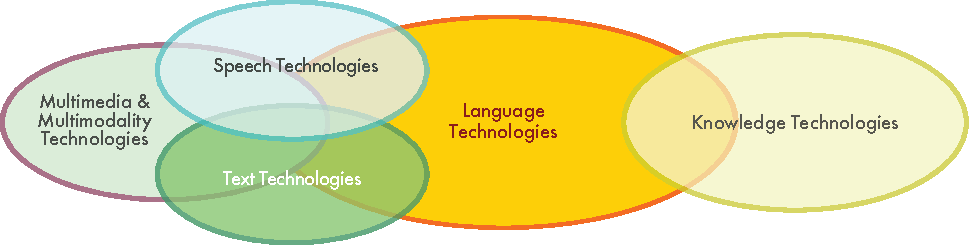
\includegraphics[width=\textwidth]{../_media/english/language_technologies}
  \caption{Language technologies}
  \label{fig:ltincontexten}
  \colorrule{grey3}{\textwidth}{1.5pt}
\end{figure*}

\subsection{Application Architectures}
\begin{figure*}[hb]
  \colorrule{grey3}{\textwidth}{1.5pt}
  \center
  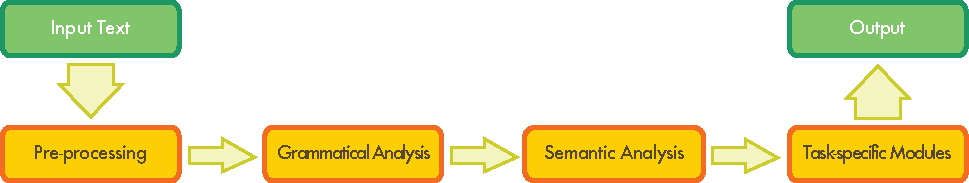
\includegraphics[width=\textwidth]{../_media/english/text_processing_app_architecture}
  \caption{A typical text processing architecture}
  \label{fig:textprocessingarch_en}
  \colorrule{grey3}{\textwidth}{1.5pt}
\end{figure*}
Typical software applications for language processing consist of several components that mirror different aspects of language and of the task they implement. Figure \ref{fig:textprocessingarch_en} displays a highly simplified architecture that can be found in a text processing system. The first three modules deal with the structure and meaning of the text input:

\begin{enumerate}
\item Pre-processing: cleans the data, analyses or removes formatting, detects the input languages, detects if the text lacks diacritics and so on.
\item Grammatical analysis: finds the verb, its objects, modifiers and other sentence elements; detects the sentence structure.
\item Semantic analysis: disambiguation (Which meaning of \emph{mier} is the right one in a given context?), resolving anaphora and referring expressions like \emph{on}, \emph{to auto}, etc.; representing the meaning of the sentence in a machine-readable way.
\end{enumerate}

Task-specific modules then perform many different operations such as
automatic summarisation of an input text, database look-ups and many
others. At the figure \ref{fig:textprocessingarch_en}, we will
illustrate core application areas and highlight their core modules.
Again, the architectures of the applications are highly simplified and
idealised, to illustrate the complexity of Language Technology
applications in a generally understandable way.

After introducing the core application areas, we will give a short
overview of the situation in language technology research and education,
concluding with an overview of past and ongoing research programs.
%FIXME please add translation
Finally, we will present an expert estimation on the
situation regarding core language technology tools and resources on a
number of dimensions such as availability, maturity, or quality. The general situation of LT for the Slovak language is summarised in figure~\ref{fig:lrlttable_en} (p.~\pageref{fig:lrlttable_en}) at the end of this chapter. This table lists all tools and resources that are boldfaced in the text. LT support for Slovak is also compared to other languages that are part of this series.

%\begin{figure*}[hb]
%  \colorrule{grey3}{\textwidth}{1.5pt}
%  \center
%  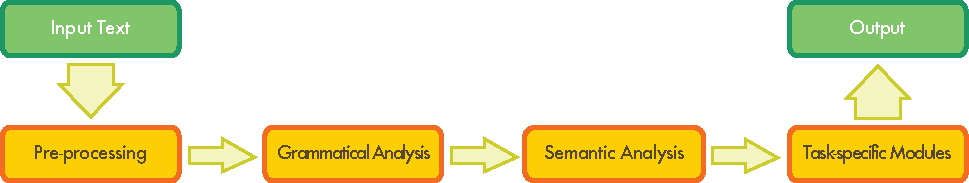
\includegraphics[width=\textwidth]{../_media/english/text_processing_app_architecture}
%  \caption{A typical text processing architecture}
%  \label{fig:textprocessingarch_en}
%  \colorrule{grey3}{\textwidth}{1.5pt}
%\end{figure*}

\subsection{Core Application Areas}
\subsubsection{Language Checking}
Anyone using a word processing tool such as Microsoft Word has come across a spell checking component that indicates spelling mistakes and proposes corrections. 40 years after the first spelling correction program by Ralph Gorin, language checkers nowadays do not simply compare the list of extracted words against a dictionary of correctly spelled words, but have become increasingly sophisticated. In addition to language-dependent algorithms for handling \underbar{morphology} (e.\,g.~plural formation), some are now capable of recognizing syntax–related errors, such as a missing verb or a verb that does not agree with its subject in person and number, e.\,g.~in ‘She *\emph{write} a letter.’ However, most available spell checkers (including Microsoft Word) will find no errors in the following first verse of a poem by Jerrold H. Zar (1992)\cite{f22}: 

\begin{verse}
\emph{%
Eye have a spelling chequer,\\
It came with my Pea Sea.\\
It plane lee marks four my revue\\
Miss Steaks I can knot sea.
}
\end{verse}

For handling these types of errors, analysis of the context is needed in many cases, e.\,g., for deciding if a word needs to be written with “y” or “i”, as in:

\begin{verse}
\emph{%
Kto chce psa biť, palicu si nájde.\\
{[}He who wants to beat a dog will find a stick.{]}\\
\smallskip
Kto chce psom byť, pána si nájde.\\
{[}He who wants to be a dog will find his master.{]}
}
\end{verse}

This either requires the formulation of language-specific \underbar{grammar} rules, i.\,e., a high degree of expertise and manual labour, or the use of a so-called statistical \underbar{language model}.  Such models calculate the probability of a particular word occurring in a specific environment (i.\,e., the preceding and following words). For example, \emph{chce psom byť} is a much more probable word sequence than \emph{chce psom biť}, and \emph{chce psa biť} is a much more probable sentence than \emph{chce psa byť} (nevertheless, we can contrive contexts where all four sequences are grammatical). A statistical language model can be automatically derived using a large amount of (correct) language data (i.\,e., a \underbar{corpus}). Up to now, these approaches have mostly been developed and evaluated on English language data. However, they do not necessarily transfer straightforwardly to Slovak with its flexible word order and richer inflection. 

\begin{figure*}[htb]
  \colorrule{grey3}{\textwidth}{1.5pt}
  \center
  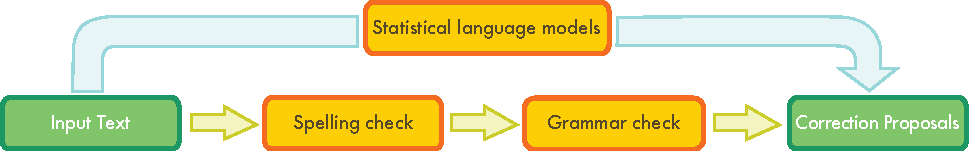
\includegraphics[width=\textwidth]{../_media/english/language_checking}
  \caption{Language checking (top: statistical; bottom: rule-based)}
  \label{fig:langcheckingaarch_en}
  \colorrule{grey3}{\textwidth}{1.5pt}
\end{figure*}

The use of Language Checking is not limited to word processing tools, but is also applied in authoring support systems. Accompanying the rising number of technical products, the amount of technical documentation has rapidly increased over the last decades. Fearing customer complaints about wrong usage and damage claims resulting from bad or badly understood instructions, companies have begun to increasingly focus on the quality of technical documentation, at the same time targeting the international market. Advances in NLP lead to the development of authoring support software, which assists the writer of technical documentation to use vocabulary and sentence structures consistent with certain rules and terminology restrictions.

\boxtext{The spelling checkers for Slovak are mostly based on a dictionary of basic word forms (lemmas)}

The existing spelling checkers for Slovak are mostly based on a dictionary of basic word forms (lemmas) combined with a set of morphological rules enabling the analysis or generation of all (correct) word forms. Although this simple approach seems to be satisfactory, it has two substantial drawbacks. The first issue concerns the superficially correct word forms appearing in a wrong context. The second drawback is the inability to distinguish between real spelling errors and word forms which are correct, but which are not contained in the dictionary. Such words will always exist due to the natural enhancement of a lexicon by newly created words, by new scientific or technical terms etc.

Besides spell checkers and authoring support, Language Checking is also important in the field of computer-assisted language learning. Language checking applications also automatically correct search engine queries, e.\,g.~Google’s ‘Did you mean\dots’ suggestions. 

\subsubsection{Web Search}

\begin{figure*}[htb]
  \colorrule{grey3}{\textwidth}{1.5pt}
  \center
  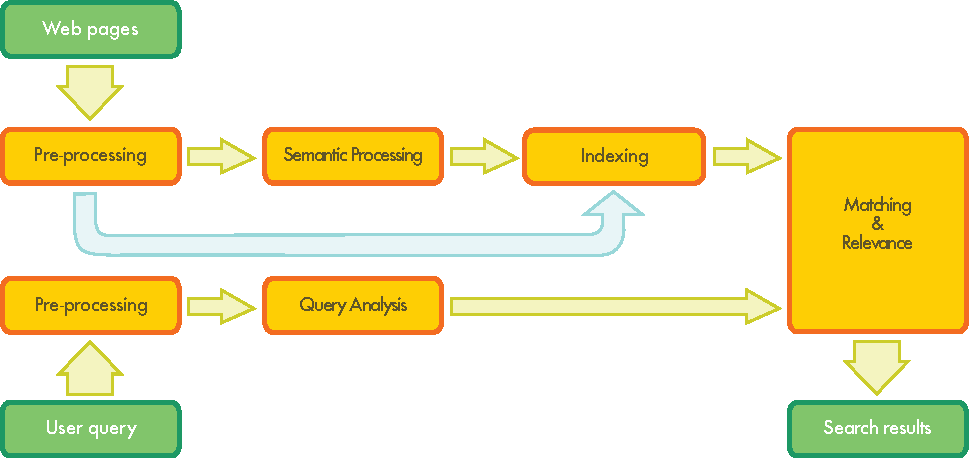
\includegraphics[width=\textwidth]{../_media/english/web_search_architecture}
  \caption{Web search architecture}
  \label{fig:websearcharch_en}
  \colorrule{grey3}{\textwidth}{1.5pt}
 \end{figure*}

Searching on the web, in intranets, or in digital libraries is probably the most widely used and yet underdeveloped Language Technology today. The search engine Google, which started in 1998, is nowadays used for about 80\% of all search queries world-wide. In 2006, the verb \emph{googlovať/googliť} very narrowly missed being included in the first volume of the new Dictionary of Contemporary Slovak Language (\emph{Slovník súčasného slovenského jazyka}), a fact that is over being used to reproach the dictionary authors for. Neither the search interface nor the presentation of the retrieved results have significantly changed since the first version. In the current version, Google offers a spelling correction for misspelled words and also, in 2009, incorporated basic semantic search capabilities into their algorithmic mix\cite{pc1}, which can improve search accuracy by analysing the meaning of the query terms in context. The success story of Google shows that with a lot of data at hand and efficient techniques for \underbar{indexing} these data, a mainly statistically-based approach can lead to satisfactory results. 

However, for a more sophisticated request for information, integrating deeper linguistic knowledge is essential. In research labs, experiments using machine-readable \underbar{thesauri} and \underbar{ontological language resources} like WordNet, have shown improvements by allowing to find a page on the basis of synonyms of the search terms, e.\,g.~\emph{jadrová}, \emph{atómová} and \emph{nukleárna energia} (nuclear, atomic and nuclear energy) or even more loosely related terms. 

\boxtext{The next generation of search engines will have to include much more sophisticated Language Technology}

The next generation of search engines will have to include much more sophisticated Language Technology. If a search query consists of a question or another type of sentence rather than a list of keywords, retrieving relevant answers to this query requires an analysis of this sentence on a syntactic and semantic level as well as the availability of an index that allows for a fast retrieval of the relevant documents. For example, imagine a user inputs the query ‘Give me a list of all companies that were taken over by other companies in the last five years’. For a satisfactory answer, syntactic \underbar{parsing} needs to be applied to analyse the grammatical structure of the sentence and determine that the user is looking for companies that have been taken over and not companies that took over others. Also, the expression \emph{last five years} needs to be processed in order to find out which years it refers to. 

Finally, the processed query needs to be matched against a huge amount of unstructured data in order to find the piece or pieces of information the user is looking for. This is commonly referred to as \underbar{information retrieval} and involves the search for and ranking of relevant documents. In addition to generating a list of companies, we also need to extract the information that a particular string of words in a document refers to a company name. This kind of information is made available by so-called \underbar{named-entity recognisers}. 

Even more demanding is the attempt to match a query to documents written in a different language. For \underbar{cross-lingual information retrieval}, we have to automatically translate the query to all possible source languages and transfer the retrieved information back to the target language. The increasing percentage of data available in non-textual formats drives the demand for services enabling \underbar{multimedia information retrieval}, i.\,e., information search on images, audio, and video data. For audio and video files, this involves a \underbar{speech recognition} module to convert speech content into text or a phonetic representation, to which user queries can be matched.

In Slovakia, there were several different small and medium enterprises (SMEs) developing search technologies, or search technologies developed by Czech SMEs were used. The first Slovak search engine taking Slovak morphology (developed at the Faculty of Mathematics and Physics, Charles University, Prague) into account was \emph{morfeo.sk}, run by the internet portal \emph{centrum.sk}, which started to provide a fulltext search of the \emph{.sk} domain webpages in 2003. It used lemmatisation and morphology annotation to look for inflected words in order to be able to provide the user with more relevant results than those including the basic forms of the words. It also included fuzzy search possibilities and search by synonyms. By 2009 the number of indexed pages was over 117 million. Since that time, Google has already included Slovak morphology support and surpassed the number of the indexed pages and \emph{centrum.sk} has switched to a customised Google Search.

One of the enterprises engaged in this field is Forma s.\,r.\,o.~\cite{f25}, a company that developed three linguistic modules: speech check, hyphenator, lemmatiser and thesaurus, on the basis of data obtained from the Ľ. Štúr Institute of Linguistics of the Slovak Academy of Sciences. The company also developed separate programs for full-text Slovak search and still operates online versions of some older dictionaries. 

Focus on development for search technologies lies in providing add-ons and advanced search engines for special-interest portals by exploiting topic-relevant semantics. Due to the still high demands in processing power, such search engines are only economically usable in relatively small text corpora. The processing time easily exceeds that of a common statistical search engine as e.\,g., provided by Google by a magnitude of thousands. These search engines also have a high demand in topic-specific domain modelling, making it infeasible to use these mechanisms on a web scale.

Research in this field is mainly performed by the Institute of Informatics of the Slovak Academy of Sciences, which started to deal with the processing of written natural language in 2006. At the same time, WIKT\cite{f26} workshops, containing several articles or even entire sections dedicated to the processing of Slovak language in each year have been initiated. Since 2006, the research in the Institute of Informatics in cooperation with Pavol Jozef Šafárik University in Košice has been mainly performed within the NAZOU\cite{f27} project aimed at the development of the tools for obtaining, processing, organizing and presenting Internet information. Job offers represented a specific application with the tools having been tested on Slovak job offers as well.  The Institute prepared an analysis of processing texts in Slovak \cite{laclavik2007a} and, at the same time, Ontea\cite{f28}, a tool for extracting of information \cite{laclavik2007b,laclavik2009} was developed. The tool was later integrated with the tools for language identification \cite{vojtek2006} and lemmatisation \cite{krajci2007}.

Ontea works on the basis of searching for patterns, which can either be linguistically dependent patterns, such as use of prepositions and sentence structure, but also simpler patterns, such as use of capitals and abbreviations e.\,g.~s.\,r.\,o. and a.\,s. for searching for businesses, \emph{SK}, \emph{SKK}, \emph{EUR}, \emph{EURO}, \emph{€} for price searching, or abbreviations of Slovak first names for searching for people in a text. A principle is applicable to various languages, but the patterns have to be made for a specific language, e.\,g.~Slovak.  At the present, the Ontea tool is being improved for use in the processing of e-mail communication. The system was tested within the AIIA project\cite{f29} \cite{laclavik2010} on Slovak e-mails from the Anasoft company and SANET association. Ontea not only uses the patterns, but also dictionaries (gazetteers) as well as their combinations in order to extract and identify entities in a text. Since the use of dictionaries (but also some patterns) can cause problems with the identification of an entity that is in other than basic form, use of lemmatiser seems to be appropriate. Since the entities are mostly of a nomenclatural nature, such as people, locations, product names, names of projects or services, they are difficult to be lemmatised. Although the problems have not yet been successfully resolved, they could be settled by a new method with the combination of dictionaries, character based tokenization, lemmatisation, and verification of an entity in a dictionary.

The extraction of entities using patterns was also used in an experiment with large group of data, when Slovak websites were processed with an aim of extraction of geographical data (Slovak addresses) and their subsequent finding \cite{dlugolinsky2010}.

\subsubsection{Speech Technology}
Speech technology is the basis for the creation of interfaces that allow a user to interact with machines using spoken language rather than with graphical display, keyboard, and mouse. Today these voice user interfaces (VUIs) are employed for partially or fully automating service offerings provided by companies to their customers, employees, or partners via telephone. Business domains that rely heavily on VUIs are banking, logistics, public transportation, and telecommunications. Other usages of Speech technology are interfaces to particular devices such as in-car navigation systems, and the employment of spoken language as an alternative to the input/output modalities of graphical user interfaces, e.\,g.~in smartphones or tablets.

\begin{figure*}[htb]
  \colorrule{grey3}{\textwidth}{1.5pt}
  \center
  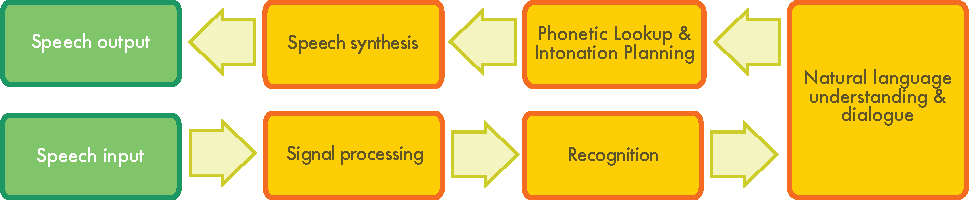
\includegraphics[width=\textwidth]{../_media/english/simple_speech-based_dialogue_architecture}
  \caption{Speech-based dialogue system}
  \label{fig:dialoguearch_en}
  \colorrule{grey3}{\textwidth}{1.5pt}
\end{figure*}

At its core, Speech technology comprises the following four different technologies:

\begin{enumerate}
\item Automatic \underbar{speech recognition} (ASR) is responsible for determining which words were actually spoken given a sequence of sounds uttered by a user.
\item \underbar{Syntactic analysis} and \underbar{semantic interpretation} deal with analysing the syntactic structure of a user’s utterance and interpreting the latter according to the purpose of the respective system.
\item \underbar{Dialogue management} is required for determining, on the part of the system the user interacts with, which action shall be taken given the user’s input and the functionality of the system.
\item \underbar{Speech synthesis} (Text-to-Speech, TTS) technology is employed for transforming the wording of that utterance into  sounds that will be output to the user. 
\end{enumerate}

One of the major challenges is to have an ASR system recognising the words uttered by a user as precisely as possible. This requires either a restriction of the range of possible user utterances to a limited set of keywords, or the manual creation of language models that cover a large range of natural language user utterances. A fundamental requirement for good performance is also a well trained acoustic model based on a huge amount of recorded data covering different accents, age groups, genders etc. Whereas the former results in a rather rigid and inflexible usage of a VUI and possibly causes a poor user acceptance, the creation, tuning and maintenance of acoustic and language models may increase the costs significantly. However, VUIs that employ language models and initially allow a user to flexibly express their intent – evoked by a ‘How may I help you’ greeting – show both a higher automation rate and higher user acceptance and may therefore be considered as advantageous over a less flexibly directed dialogue approach. An exception to the above mentioned are  so-called embedded systems. They require a  small set of commands and the usage of language models in such cases is a disadvantage. Embedded systems are today still successfully built with grammars. 

For the output part of a VUI, companies tend to use utterances pre-recorded by professional – ideally corporate – speakers a lot. Static utterances in which the wording does not depend on the particular contexts of use or the personal data of the given users will result in a rich user experience. However, the more dynamic the content an utterance needs to consider, the more the user experience may suffer from a poor prosody resulting from concatenating single audio files. In contrast, today’s TTS systems prove superior, though optimizable, regarding the prosodic naturalness of dynamic utterances.  

Regarding the market for Speech technology, the last decade underwent a strong standardisation of the interfaces between the different technology components, as well as by standards for creating particular software artefacts for a given application. There also has been strong market consolidation in the last ten years, particularly in the field of ASR and TTS. Here, the national markets in the G20 countries – i.\,e., economically strong countries with a considerable population - are dominated by few big players worldwide led mainly by Nuance, Google and Microsoft. 

Speech recognition in Slovakia has a long history but has been done only at universities or scientific institutions. Most places focus on basic research and solutions of specific problems of speech recognition. The Department of Speech Analysis and Synthesis of the Institute of Informatics of the Slovak Academy of Sciences as a participant of the SpeechDat-E project focuses mainly on acoustic models for telephony systems. With a growing number of speech data such as for example parliamentary discussions the institute is using existing tools for speech recognition to try to create widely usable acoustic models for applications such as dictation, talk transcription, etc. with focus on speaker dependent systems. The main focus of the Department of Telecommunication of the Slovak Technical University in Bratislava is the processing of speech signals in noisy conditions (speech/silence detection, features extraction, etc.). Among others, the department created several small speech recognition systems to compare the performance and usability of different free speech recognition systems for the Slovak language. At the Technical University of Košice there are several departments focusing on automatic speech recognition. The Department of Electronics and Multimedia Communications, which was originally focused mainly on basic research for the digital processing of speech signals, has gradually extended its research focus toward developing complex interactive speech systems. A few years ago in cooperation with research teams from the Slovak Academy of Sciences, Slovak University of Technology and University of Žilina the Smart Speech Communication System was developed at the Department of Electronics and Multimedia Communications. The system is available to public and continually serves as a demonstrator of the speech interactive services in Slovak over the telephone. Today one of the most noticeable outputs represents the activities in the field of language modelling for the Slovak large vocabulary continuous speech recognition system. The language model created at the department is based on a corpus of $2\cdot 10^9$ tokens. 
\newline The second important workplace at the Technical University of Košice is the Department of Cybernetics and Artificial Intelligence where the first voice retrieval information dialogue system and SAMPA for the Slovak language were created. Today the speech recognition activities at the department plays a rather minor role. The Department of Applied Mathematics and Statistics of the Faculty of Mathematics, Physics and Informatics at Comenius University in Bratislava is working mainly on speech recognition of isolated words for children's voices. The results were applied in an educational process to verify a text read by children. From the audio data recorded for the acoustic model training two speech databases have been created (\emph{Alica} and \emph{Viktória}).  The main institution for speech recognition at the University of Žilina is the Department of Telecommunications and Multimedia. Its team focuses mainly on digital signal processing for speech recognition and recognition of isolated words using Hidden Markov Models.

Close cooperation between the Department of Electronics and Multimedia Communications of the Technical University of Košice and the Department of Speech Analysis and Synthesis of the Institute of Informatics of the Slovak Academy of Sciences resulted in the first visible success in developing the Slovak large vocabulary continuous speech recognition system. The result of the cooperation is an automatic speech dictation system commercially usable in judiciary.

Regarding commercial systems for Slovak speech recognition, it is worth mentioning the product from Newton Technology Company. It can be considered as the first usable speaker independent dictation system for the Slovak language.

Looking beyond today’s state of technology, there will be significant changes due to the spread of smartphones as a new platform for managing customer relationships – in addition to the telephone, internet, and email channels. This tendency will also affect the employment of technology for Speech Interaction. On one hand, demand for telephony-based VUIs will decrease in long run. On the other hand, the usage of spoken language as a user-friendly input modality for smartphones will gain significant importance. This tendency is supported by the observable improvement of speaker-independent speech recognition accuracy for speech dictation services that are already offered as centralised services to smartphone users. Given this ‘outsourcing’ of the recognition task to the infrastructure of applications, the application-specific employment of linguistic core technologies will supposedly gain importance compared to the present situation. 

\subsubsection{Machine Translation}

\begin{figure*}[htb]
  \colorrule{grey3}{\textwidth}{1.5pt}
  \center
  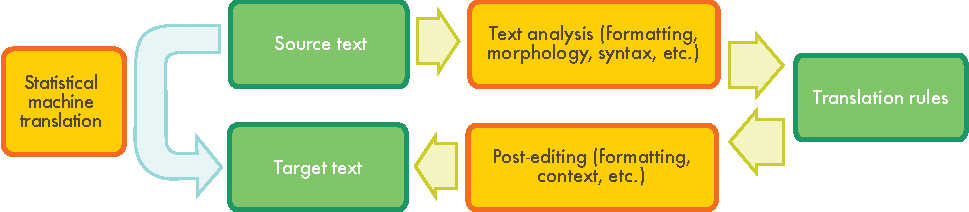
\includegraphics[width=\textwidth]{../_media/english/machine_translation}
  \caption{Machine translation (left: statistical; right: rule-based)}
  \label{fig:mtarch_en}
  \colorrule{grey3}{\textwidth}{1.5pt}
\end{figure*}

The idea of using digital computers for the translation of natural languages came up in 1946 by A. D. Booth and was followed by substantial funding for research in this area in the 1950s and beginning again in the 1980s. Nevertheless, \underbar{Machine Translation} (MT) still fails to fulfil the high expectations it gave rise to in its early years. 

At its basic level, MT simply substitutes words in one natural language with words in another. This can be useful in subject domains with a very restricted, formulaic language, e.\,g., weather reports. However, for a good translation of less standardised texts, larger text units (phrases, sentences, or even whole passages) need to be matched to their closest counterparts in the target language. The major difficulty here lies in the fact that human language is ambiguous, which yields challenges on multiple levels, e.\,g., \underbar{word sense disambiguation} at the lexical level (‘Leopard’ can mean an animal or an operating system) or the attachment of attributes on the syntactic level as in:

\begin{verse}
\emph{Otcovi priatelia neprišli, moji áno.}\\
{[}Father's friends did not come, mine did.{]}\\
\smallskip
\emph{Otcovi priatelia neprišli, mne áno.}\\
{[}The friends did not come to the father, {[}but{]} to me.{]}
\end{verse}

One way of approaching the task is based on linguistic rules. For translations between closely related languages, a direct translation may be feasible in cases like the example above. But often, rule-based (or knowledge-driven) systems analyse the input text and create an intermediary, symbolic representation from which the text in the target language is generated. The success of these methods is highly dependent on the availability of extensive \underbar{lexicons} with morphological, syntactic and semantic information as well as large sets of \underbar{grammar} rules carefully designed by a skilled linguist.

Beginning in the late 1980s, as computational power increased and became less expensive, more interest was shown in statistical models for MT. The parameters of these statistical models are derived from the analysis of bilingual text \underbar{corpora} such as the Europarl parallel corpus, which contains the proceedings of the European Parliament in 21 European languages. Given enough data, statistical MT works well enough to derive an approximate meaning of a foreign language text. However, unlike knowledge-driven systems, statistical (or data-driven) MT often generates ungrammatical output. On the other hand, besides the advantage that less human effort is required for grammar writing, data-driven MT can also cover particularities of the language that go missing in knowledge-driven systems, for example idiomatic expressions. 

As the strengths and weaknesses of knowledge- and data-driven MT are complementary, researchers nowadays unanimously target hybrid approaches by combining the methodologies of both. This can be done in several ways. One is to use both knowledge-driven and data-driven systems and have a selection module decide on the best output for each sentence. However, for longer sentences, no result will be perfect. A better solution is to combine the best parts of each sentence from multiple outputs, which can be fairly complex, as corresponding parts of multiple alternatives are not always obvious and need to be aligned. 

In the 1990s a prototype of MT between closely related languages was proposed for the pair Czech and Slovak at Charles University in Prague.

TEOS Trenčín markets the first practical multilingual MT software for the Slovak language, bundled with their PC dictionary software. However, since the system did not use any further linguistic analysis and simply substituted words from one language with words in the other language (mostly limited to lemmas), its usability was limited to languages that do not have much morphology – i.\,e.~English. A later version allowed to translate webpages on the fly, a functionality that is particularly useful in the English$\rightarrow$Slovak translation, which coincidentally was the only translation direction that “worked”.

The quality of MT systems is still considered to have a huge improvement potential. Challenges include the adaptability of the language resources to a given subject domain or user area and the integration into existing workflows with term bases and translation memories. In addition, most of the current systems (not limited to the Slovak language) are English-centred. In particular, Google Translator offers the best translation quality for translations from/to English.

\boxtext{The quality of MT systems is still considered to have a huge improvement potential}

The availability of large amounts of bilingual texts is really the key in statistical MT. For Slovak, corpora of parallel texts with several other languages are currently being created. The largest data – in total several million pairs of sentences – is available in the Slovak-Czech and Slovak-English parallel corpora compiled at the Ľ. Štúr Institute of Linguistics. The corpora contain mostly fiction and are automatically sentence aligned.

%FIXME please add translation
Figure~\ref{fig:euromatrix_en} (p.~\pageref{fig:euromatrix_en}), which was prepared during the EC Euromatrix+ project, shows the pair-wise performances obtained for 22 of the 23 official EU languages (Irish was not compared). The results are ranked according to a BLEU score, which indicates higher scores for better translations \cite{bleu1}. A human translator would normally achieve a score of around 80 points.

\subsection{Other Application Areas}
Building Language Technology applications involves a range of subtasks that do not always surface at the level of interaction with the user, but provide significant service functionalities ‘under the hood’ of the system. Therefore, they constitute important research issues that have become individual sub-disciplines of Computational Linguistics in academia. 

\underbar{Question answering} has become an active area of research, for which annotated \underbar{corpora} have been built and scientific competitions have been started. The idea is to move from a keyword-based search (to which the engine responds with a whole collection of potentially relevant documents) to the scenario of the user asking a concrete question and the system providing a single answer:
\begin{itemize}
	\item[] \textit{Question: How old was Neil Armstrong when he stepped on the moon?}
	\item[] \textit{Answer: 38.}
\end{itemize}
While this is obviously related to the aforementioned core area Web Search, question answering nowadays is primarily an umbrella term for research questions such as what \emph{types} of questions should be distinguished and how they should be handled, how a set of documents that potentially contain the answer can be analysed and compared (do they give conflicting answers?), and how specific information – the answer – can be reliably extracted from a document, without unduly ignoring the context. 

This is in turn related to the \underbar{information extraction} (IE) task, an area that was extremely popular and influential at the time of the ‘statistical turn’ in Computational Linguistics in the early 1990s. IE aims at identifying specific pieces of information in specific classes of documents; this could be e.\,g.~the detection of the key players in company takeovers as reported in newspaper stories. Another scenario that has been worked on is reports on terrorist incidents, where the problem is to map the text to a template specifying the perpetrator, the target, time and location of the incident and the results of the incident. Domain-specific template-filling is the central characteristic of IE, which for this reason is another example of a ‘behind the scenes’ technology that constitutes a well-demarcated research area but for practical purposes then needs to be embedded into a suitable application environment. 

The JBOWL (Java Bag-Of-Words Library) software library was developed at the Centre for Information Technologies (FEI-CIT) in Košice for the support of NLP and Text Mining applications. JBOWL is a modular system enabling the maintenance of textual documents. It provides functions and the means of supporting the processing of natural language texts (e.\,g., tokenization, morphological analysis, lemmatisation, disambiguation, syntactic analysis based on ATN networks, clustering and phrase identification, term weighting and indexing) as well as the knowledge discovery and mining from unstructured textual documents. In addition, the system provides implementations of several algorithms of controlled and uncontrolled machine learning with customizable input parameters and methods for evaluating the quality of Text Mining models.

\boxtext{The software library was developed at the Centre for Information Technologies in Košice to maintain textual documents}

Two ‘borderline’ areas, which sometimes play the role of a standalone application and sometimes that of a supportive, ‘under the hood’ component are \underbar{text summarisation} and \underbar{text generation}. Summarisation, obviously, refers to the task of making a long text short, and is offered for instance as a functionality within MS Word. It works largely on a statistical basis by first identifying ‘important’ words in a text (that is, for example, words that are highly frequent in this text but markedly less frequent in general language use) and then determining those sentences that contain many important words. These sentences are then marked in the document, or extracted from it, and are taken to constitute the summary. In this scenario, which is by far the most popular one, summarisation equals sentence extraction: the text is reduced to a subset of its sentences. All commercial summarisers make use of this idea. An alternative approach, to which some research is devoted, is to actually synthesise \emph{new} sentences, i.\,e., to build a summary of sentences that need not show up in that form in the source text. This requires a certain amount of deeper understanding of the text and therefore is much less robust. All in all, a text generator is in most cases not a stand-alone application but embedded into a larger software environment such as a clinical information system where patient data is collected, stored and processed, and report generation is just one of many functions.

\subsection{Language Technology in Education}
Language Technology is a highly interdisciplinary field involving the expertise of linguists, computer scientists, mathematicians, philosophers, psycholinguists, and neuroscientists among others. As such, it has not yet acquired a fixed place in the Slovak faculty system.

\boxtext{The course on information retrieval, information extraction, graph algorithms for their support and processing large amounts of data has been taken at the Institute of Informatics}

Since 2007 the researchers from the Institute of Informatics of the Slovak Academy of Sciences (Michal Laclavík and Martin Šeleng) have been teaching the Information retrieval course\cite{f30} at the Faculty of Information Technologies of the Slovak Technical University. This course focuses on such themes as information retrieval, information extraction, graph algorithms for their support as well as processing large amounts of data. The students solve various practical projects in this domain, while many of them use Slovak text sources, and some of them directly solve the NLP problems of Slovak language processing. As an example, let us mention several projects aimed at the creation of a statistical, dictionary-oriented or algorithmic stemmer based on the  “snowball” or “Egothor” projects, and at the determination of the efficiency and statistics for the simple stemmers which function on the principle of omitting the vowels, diacritic marks or, eventually, word endings etc. At the same time, there are also statistical translation projects or the automatic dictionary creation between the Slovak or other languages (English, Czech). Finally, let us mention the projects utilising dictionaries or frequency language dictionaries for applications such as T9, named entities extraction using computer learning methods and libraries such as OpenNLP, the creation of POS tagging algorithms as well as the extraction of events from e-mails or from Slovak webpages and the like.

There is no regular Computational Linguistics study programme otherwise.

\subsection{National Projects and Initiatives}
In Slovakia, the language technologies and their development are still considered mostly a scientific
area and are included predominantly in applied research, either linguistic
(particularly lexicography) or computer science. The connection with the
business sector has been rather weak and sporadic. However, recently the
language technologies have been making strong and resolute entrance to many
software applications.

The first two big government funded research projects with a focus on language
technologies and resources in Slovakia were \emph{National Corpus of the Slovak Language and
Electronisation of Linguistic Research in the years 2002--2006} and \emph{Integrated Computational
Processing of the Slovak Language for Linguistic Research Purposes}, both
carried out at Ľ. Štúr Institute of Linguistics, Slovak Academy of Sciences.

\emph{National Corpus of the Slovak Language and Electronisation of Linguistic
Research in years 2002--2006}, approved by a government resolution n.
137/2002, was aimed at building a representative corpus of Slovak language, as a necessary foundation
and data source for any linguistic and natural language processing research.
The corpus data form the base in compiling the comprehensive Dictionary of
Contemporary Slovak.


In this project, the Slovak National Corpus Department was created and
subsequently became the leading institution in NLP research in Slovakia. The
project continued in its 2\textsuperscript{nd} period as \emph{Construction of Slovak National Corpus and Electronisation of Linguistic Research in Slovakia} (in the years 2007--2011) as agreed by the Ministry of Education of the Slovak Republic, Ministry of Culture of the Slovak Republic and the Slovak Academy of Sciences.


The project \emph{Integrated Computational Processing of the Slovak Language for Linguistic
Research Purposes}, n. 2003SP200280307 was carried out in years 2003--2006 in the frame of the State research and development programme \emph{Current Issues in Society Development}. The project supplemented the Slovak language resources with necessary tools and additional data (morphological a stylistic annotation, electronic linguistic resources, terminology database etc.). The results of the project are further used in subsequent projects and also in commercial environment.


Another major project concerning the Slovak language processing was the project
\emph{Automatic Transcription of Dictate for the Ministry of Justice of
the Slovak Republic},  coordinated by the Department of Speech Analysis
and Synthesis of the Institute of Informatics of the Slovak Academy of
Sciences, with participation of the Department of Electronics and
Multimedia Communications of the Technical University of Košice,
carried out in the years 2009--2011. The goal of the project was to
create a complete system for transcribing spoken Slovak language,
specialised for judicial domain. The project has been funded by the
Ministry of Justice of the Slovak Republic, and is currently being
deployed commercially in the courts of law throughout the Slovak
Republic.

These three projects were so far the only major initiatives concerning natural
language processing of the Slovak language. They paved the way for further
research and commercial projects, but the need for additional research and its funding is clearly necessary.

\subsection{Availability of Tools and Resources}
The figure \ref{fig:lrlttable_en} summarises the current state of language technology support for the Slovak language. The rating for existing tools and resources was generated by leading experts in the field who provided estimates based on a scale from 0 (very low) to 6 (very high) according to seven criteria.

\begin{figure*}[htb]
\centering

\begin{tabular}{>{\columncolor{orange1}}p{.33\linewidth}@{\hspace*{6mm}}c@{\hspace*{6mm}}c@{\hspace*{6mm}}c@{\hspace*{6mm}}c@{\hspace*{6mm}}c@{\hspace*{6mm}}c@{\hspace*{6mm}}c}
\rowcolor{orange1}
 \cellcolor{white}&
 \begin{sideways}\makecell[l]{Quantity}\end{sideways} &
 \begin{sideways}\makecell[l]{\makecell[l]{Availability} }\end{sideways} &
 \begin{sideways}\makecell[l]{Quality}\end{sideways} &
 \begin{sideways}\makecell[l]{Coverage}\end{sideways} &
 \begin{sideways}\makecell[l]{Maturity}\end{sideways} &
 \begin{sideways}\makecell[l]{Sustainability~~~}\end{sideways} &
 \begin{sideways}\makecell[l]{Adaptability}\end{sideways} \\ \addlinespace

\multicolumn{8}{>{\columncolor{orange2}}l}{\textcolor{black}{Language Technology: Tools, Technologies and Applications}} \\ \addlinespace

Speech Recognition	&3	&1	&2	&2	&3	&3	&2 \\ \addlinespace
Speech Synthesis 	&3	&3	&3	&3	&3	&3	&3 \\ \addlinespace
Grammatical analysis 	&2	&2	&3	&2	&2	&3	&3 \\ \addlinespace
Semantic analysis 	&1	&2	&1	&1	&1	&3	&3 \\ \addlinespace
Text generation 	&1	&1	&1	&1	&0	&1	&1 \\ \addlinespace
Machine translation 	&2	&2	&2	&2	&2	&1	&2 \\ \addlinespace

\multicolumn{8}{>{\columncolor{orange2}}l}{\textcolor{black}{Language Resources: Resources, Data and Knowledge Bases}} \\ \addlinespace

Text corpora 		&2	&4	&4	&5	&4	&4	&4 \\ \addlinespace
Speech corpora 		&3	&4	&2	&2	&3	&3	&3 \\ \addlinespace
Parallel corpora 	&2	&3	&2	&2	&2	&2	&3 \\ \addlinespace
Lexical resources 	&3	&2	&3	&4	&3	&4	&3 \\ \addlinespace
Grammars 		&2	&3	&3	&2	&1	&2	&1 \\
\end{tabular}
\caption{State of language technology support for Slovak}
\label{fig:lrlttable_en}
\end{figure*}

\begin{enumerate}
\item Quantity: Does a tool/resource exist for the language at hand? The more tools/resources exist, the higher the rating.
\begin{itemize}
\item 0: no tools/resources whatsoever
\item 6: many tools/resources, large variety
\end{itemize}
\item Availability: Are tools/resources accessible, i.\,e.,are they Open Source, freely usable on any platform or only available for a high price or under very restricted conditions?
\begin{itemize}
\item 0: practically all tools/resources are only available for a high price
\item 6: a large amount of tools/resources is freely, openly available under sensible Open Source or Creative Commons licenses that allow re-use and re-purposing (If there are e.\,g.,~two resources, one of them completely open and the other completely closed, we put the average (i.\,e.,~3))
\end{itemize}
\item Quality: How well are the respective performance criteria of tools and quality indicators of resources met by the best available tools, applications or resources? Are these tools/resources current and also actively maintained?
\begin{itemize}
\item 0: toy resource/tool
\item 6: high-quality tool, human-quality annotations in a resource
\end{itemize}
\item Coverage: To what degree do the best tools meet the respective coverage criteria (styles, genres, text sorts, linguistic phenomena, types of input/output, number of languages supported by an MT system etc.)? To what degree are resources representative of the targeted language or sublanguages?
\begin{itemize}
\item 0: special-purpose resource or tool, specific case, very small coverage, only to be used for very specific, non-general use cases
\item 6: very broad coverage resource, very robust tool, widely applicable, many languages supported
\end{itemize}
\item Maturity: Can the tool/resource be considered mature, stable, ready for the market? Can the best available tools/resources be used out-of-the-box or do they have to be adapted? Is the performance of such a technology adequate and ready for production use or is it only a prototype that cannot be used for production systems? An indicator may be whether resources/tools are accepted by the community and successfully used in LT systems. 
\begin{itemize}
\item 0: preliminary prototype, toy system, proof-of-concept, example resource exercise
\item 6: immediately integratable/applicable component
\end{itemize}
\item Sustainability: How well can the tool/resource be maintained/integrated into current IT systems? Does the tool/resource fulfill a certain level of sustainability concerning documentation/manuals, explanation of use cases, front-ends, GUIs etc.? Does it use/employ standard/best-practice programming environments (such as Java EE)? Do industry/research standards/quasi-standards exist and if so, is the tool/resource compliant (data formats etc.)?
\begin{itemize}
\item 0: completely proprietary, ad hoc data formats and APIs
\item 6: full standard-compliance, fully documented
\end{itemize}
\item Adaptability: How well can the best tools or resources be adapted/extended to new tasks/domains/genres/text types/use cases etc.?
\begin{itemize}
\item 0: practically impossible to adapt a tool/resource to another task, impossible even with large amounts of resources or person months at hand
\item 6: very high level of adaptability; adaptation also very easy and efficiently possible
\end{itemize}
\end{enumerate}

The key results for the Slovak language can be summed up as follows:

\begin{itemize}
\item While some specific corpora of high quality exist, a very large syntactically annotated corpus is not available.
\item For Slovak, the Slovak National Corpus is the reference language corpus, but only the query interface is generally available, due to licensing restrictions.
\item On the other hand, the Corpus of Spoken Slovak is not encumbered by copyright law and is therefore publicly available, but its size is minuscule compared to the corpus of written language.
\item Many of the resources lack standardisation, i.\,e., even if they exist, sustainability is not given; concerted programs and initiatives are needed to standardise data and interchange formats.
\item Semantics is more difficult to process than syntax; text semantics is more difficult to process than word and sentence semantics.
\item There is an ontological resource for Slovak (even mapped to English ontological resources) but its coverage is limited.
\item Standards do exist for semantics in the sense of world knowledge (RDF, OWL, etc.); they are, however, not easily applicable to NLP tasks.
\item Written text processing is more mature than speech processing (especially speech recognition)
\item Many of the resources taken as standard in other languages are missing for Slovak; NLP language research in Slovakia is severely underfunded.
\item Some of the research and development activities for the Slovak language is carried out in the Czech Republic by Czech universities and Czech SMEs.
\item Speech Recognition of the Slovak language is studied at several universities and workplaces but the amount of free tools and data is limited.
\item In contrast with speech recognition, speech synthesis is less covered by universities and other workplaces.
\item In the field of speech synthesis, there are open source packages available together with several other simple synthesizers but the speech synthesis with more natural voices is not available.
\item Slovak dialogue systems are not extended due to the poor accessibility of high quality speech recognition modules of the Slovak language.
\end{itemize}

\subsection{Cross-language Comparison}

The current state of LT support varies considerably from one language community to another. In order to compare the situation between languages, this section will present an evaluation based on two sample application areas (machine translation and speech processing) and one underlying technology (text analysis), as well as basis resources needed for building LT applications. The languages were categorised using the following five-point scale:

% Cluster 1
\begin{figure*}[h!]
  \small
  \centering
  \begin{tabular}
  { % defines color for each column.
  >{\columncolor{corange5}}p{.13\linewidth}@{\hspace{.040\linewidth}}
  >{\columncolor{corange4}}p{.13\linewidth}@{\hspace{.040\linewidth}}
  >{\columncolor{corange3}}p{.13\linewidth}@{\hspace{.040\linewidth}}
  >{\columncolor{corange2}}p{.13\linewidth}@{\hspace{.040\linewidth}}
  >{\columncolor{corange1}}p{.13\linewidth} 
  }
  \multicolumn{1}{>{\columncolor{white}}c@{\hspace{.040\linewidth}}}{\textbf{Excellent}} & 
  \multicolumn{1}{@{}>{\columncolor{white}}c@{\hspace{.040\linewidth}}}{\textbf{Good}} &
  \multicolumn{1}{@{}>{\columncolor{white}}c@{\hspace{.040\linewidth}}}{\textbf{Moderate}} &
  \multicolumn{1}{@{}>{\columncolor{white}}c@{\hspace{.040\linewidth}}}{\textbf{Fragmentary}} &
  \multicolumn{1}{@{}>{\columncolor{white}}c}{\textbf{Weak/no}} \\ 
  \multicolumn{1}{>{\columncolor{white}}c@{\hspace{.040\linewidth}}}{\textbf{support}} & 
  \multicolumn{1}{@{}>{\columncolor{white}}c@{\hspace{.040\linewidth}}}{\textbf{support}} &
  \multicolumn{1}{@{}>{\columncolor{white}}c@{\hspace{.040\linewidth}}}{\textbf{support}} &
  \multicolumn{1}{@{}>{\columncolor{white}}c@{\hspace{.040\linewidth}}}{\textbf{support}} &
  \multicolumn{1}{@{}>{\columncolor{white}}c}{\textbf{support}} \\ \addlinespace
  & \vspace*{0.5mm}English
& \vspace*{0.5mm}German \newline   
Italian \newline  
Finnish \newline 
French \newline 
Dutch \newline 
Portuguese \newline 
Spanish \newline
Czech \newline 
& \vspace*{0.5mm}Basque \newline 
Bulgarian \newline 
Danish \newline 
Estonian \newline 
Galician\newline 
Greek \newline  
Irish \newline  
Catalan \newline 
Norwegian \newline 
Polish \newline 
Swedish \newline
Serbian \newline 
\textbf{Slovak} \newline 
Slovene \newline 
Hungarian  \newline
& \vspace*{0.5mm}Icelandic \newline  
Croatian \newline 
Latvian \newline 
Lithuanian \newline 
Maltese \newline 
Romanian\\
\end{tabular}
\label{fig:speech_cluster_en}
\caption{Language clusters for Speech Processing}
\end{figure*}
  
% Cluster 2
\begin{figure*}[htb]
  \small
  \centering
  \begin{tabular}
  { % defines color for each column.
  >{\columncolor{corange5}}p{.13\linewidth}@{\hspace{.040\linewidth}}
  >{\columncolor{corange4}}p{.13\linewidth}@{\hspace{.040\linewidth}}
  >{\columncolor{corange3}}p{.13\linewidth}@{\hspace{.040\linewidth}}
  >{\columncolor{corange2}}p{.13\linewidth}@{\hspace{.040\linewidth}}
  >{\columncolor{corange1}}p{.13\linewidth} 
  }
  \multicolumn{1}{>{\columncolor{white}}c@{\hspace{.040\linewidth}}}{\textbf{Excellent}} & 
  \multicolumn{1}{@{}>{\columncolor{white}}c@{\hspace{.040\linewidth}}}{\textbf{Good}} &
  \multicolumn{1}{@{}>{\columncolor{white}}c@{\hspace{.040\linewidth}}}{\textbf{Moderate}} &
  \multicolumn{1}{@{}>{\columncolor{white}}c@{\hspace{.040\linewidth}}}{\textbf{Fragmentary}} &
  \multicolumn{1}{@{}>{\columncolor{white}}c}{\textbf{Weak/no}} \\ 
  \multicolumn{1}{>{\columncolor{white}}c@{\hspace{.040\linewidth}}}{\textbf{support}} & 
  \multicolumn{1}{@{}>{\columncolor{white}}c@{\hspace{.040\linewidth}}}{\textbf{support}} &
  \multicolumn{1}{@{}>{\columncolor{white}}c@{\hspace{.040\linewidth}}}{\textbf{support}} &
  \multicolumn{1}{@{}>{\columncolor{white}}c@{\hspace{.040\linewidth}}}{\textbf{support}} &
  \multicolumn{1}{@{}>{\columncolor{white}}c}{\textbf{support}} \\ \addlinespace
  & \vspace*{0.5mm} English 
& \vspace*{0.5mm} French \newline 
Spanish
& \vspace*{0.5mm}German \newline 
Italian \newline 
Catalan \newline 
Dutch \newline 
Polish \newline 
Romanian \newline 
Hungarian 
& \vspace*{0.5mm}Basque \newline 
Bulgarian \newline 
Danish \newline 
Estonian \newline 
Finnish \newline 
Galician \newline 
Greek \newline 
Irish \newline 
Icelandic \newline 
Croatian \newline 
Latvian \newline 
Lithuanian \newline 
Maltese \newline 
Norwegian \newline 
Portuguese \newline 
Swedish \newline 
Serbian \newline 
\textbf{Slovak} \newline 
Slovene \newline 
Czech \newline
\end{tabular}
\label{fig:mt_cluster_en}
\caption{Language clusters for Machine Translation}
\end{figure*}
  
% Cluster 3
\begin{figure*}[htb]
  \small
  \centering
  \begin{tabular}
  { % defines color for each column.
  >{\columncolor{corange5}}p{.13\linewidth}@{\hspace{.040\linewidth}}
  >{\columncolor{corange4}}p{.13\linewidth}@{\hspace{.040\linewidth}}
  >{\columncolor{corange3}}p{.13\linewidth}@{\hspace{.040\linewidth}}
  >{\columncolor{corange2}}p{.13\linewidth}@{\hspace{.040\linewidth}}
  >{\columncolor{corange1}}p{.13\linewidth} 
  }
  \multicolumn{1}{>{\columncolor{white}}c@{\hspace{.040\linewidth}}}{\textbf{Excellent}} & 
  \multicolumn{1}{@{}>{\columncolor{white}}c@{\hspace{.040\linewidth}}}{\textbf{Good}} &
  \multicolumn{1}{@{}>{\columncolor{white}}c@{\hspace{.040\linewidth}}}{\textbf{Moderate}} &
  \multicolumn{1}{@{}>{\columncolor{white}}c@{\hspace{.040\linewidth}}}{\textbf{Fragmentary}} &
  \multicolumn{1}{@{}>{\columncolor{white}}c}{\textbf{Weak/no}} \\ 
  \multicolumn{1}{>{\columncolor{white}}c@{\hspace{.040\linewidth}}}{\textbf{support}} & 
  \multicolumn{1}{@{}>{\columncolor{white}}c@{\hspace{.040\linewidth}}}{\textbf{support}} &
  \multicolumn{1}{@{}>{\columncolor{white}}c@{\hspace{.040\linewidth}}}{\textbf{support}} &
  \multicolumn{1}{@{}>{\columncolor{white}}c@{\hspace{.040\linewidth}}}{\textbf{support}} &
  \multicolumn{1}{@{}>{\columncolor{white}}c}{\textbf{support}} \\ \addlinespace
  & \vspace*{0.5mm}English
& \vspace*{0.5mm}German \newline 
  French \newline 
  Italian \newline 
  Dutch \newline 
  Spanish
& \vspace*{0.5mm}Basque \newline 
  Bulgarian \newline 
  Danish \newline 
  Finnish \newline 
  Galician \newline 
  Greek \newline 
  Catalan \newline 
  Norwegian \newline 
  Polish \newline 
  Portuguese \newline 
  Romanian \newline 
  Swedish \newline 
  \textbf{Slovak} \newline 
  Slovene \newline 
  Czech \newline 
  Hungarian \newline 
& \vspace*{0.5mm}Estonian \newline 
  Irish \newline 
  Icelandic \newline 
  Croatian \newline 
  Latvian \newline 
  Lithuanian \newline 
  Maltese \newline 
  Serbian \\
  \end{tabular}
\label{fig:text_cluster_en}
\caption{Language clusters for Text Analysis}
\end{figure*}
  
% Cluster 4
\begin{figure*}[htb]
  \small
  \centering
  \begin{tabular}
  { % defines color for each column.
  >{\columncolor{corange5}}p{.13\linewidth}@{\hspace{.040\linewidth}}
  >{\columncolor{corange4}}p{.13\linewidth}@{\hspace{.040\linewidth}}
  >{\columncolor{corange3}}p{.13\linewidth}@{\hspace{.040\linewidth}}
  >{\columncolor{corange2}}p{.13\linewidth}@{\hspace{.040\linewidth}}
  >{\columncolor{corange1}}p{.13\linewidth} 
  }
  \multicolumn{1}{>{\columncolor{white}}c@{\hspace{.040\linewidth}}}{\textbf{Excellent}} & 
  \multicolumn{1}{@{}>{\columncolor{white}}c@{\hspace{.040\linewidth}}}{\textbf{Good}} &
  \multicolumn{1}{@{}>{\columncolor{white}}c@{\hspace{.040\linewidth}}}{\textbf{Moderate}} &
  \multicolumn{1}{@{}>{\columncolor{white}}c@{\hspace{.040\linewidth}}}{\textbf{Fragmentary}} &
  \multicolumn{1}{@{}>{\columncolor{white}}c}{\textbf{Weak/no}} \\ 
  \multicolumn{1}{>{\columncolor{white}}c@{\hspace{.040\linewidth}}}{\textbf{support}} & 
  \multicolumn{1}{@{}>{\columncolor{white}}c@{\hspace{.040\linewidth}}}{\textbf{support}} &
  \multicolumn{1}{@{}>{\columncolor{white}}c@{\hspace{.040\linewidth}}}{\textbf{support}} &
  \multicolumn{1}{@{}>{\columncolor{white}}c@{\hspace{.040\linewidth}}}{\textbf{support}} &
  \multicolumn{1}{@{}>{\columncolor{white}}c}{\textbf{support}} \\ \addlinespace
  & \vspace*{0.5mm}English
& \vspace*{0.5mm}German \newline 
    French \newline 
    Dutch \newline 
    Swedish \newline 
    Czech \newline 
    Polish \newline
    Hungarian \newline
    Italian \newline
    Spanish
& \vspace*{0.5mm} Basque\newline 
    Bulgarian\newline 
    Danish \newline 
    Estonian \newline 
    Finnish \newline 
    Galician \newline 
    Greek \newline 
    Catalan \newline 
    Croatian \newline 
    Norwegian \newline 
    Portuguese \newline 
    Romanian \newline 
    Serbian \newline 
    \textbf{Slovak} \newline 
    Slovene \newline
&  \vspace*{0.5mm} Irish \newline 
    Icelandic \newline 
    Latvian \newline 
    Lithuanian \newline 
    Maltese  \\
  \end{tabular}
  \caption{Language clusters for Resources}
  \label{fig:resources_cluster_en}
\end{figure*}

  
\begin{enumerate}
  \item excellent support
  \item good support
  \item moderate support
  \item fragmentary support
  \item weak or no support
\end{enumerate}

LT support was measured according to the following criteria:
\begin{itemize}
\item Speech Processing: Quality of existing speech recognition technologies, quality of existing speech synthesis technologies, coverage of domains, number and size of existing speech corpora, amount and variety of available speech-based applications
\item Machine Translation: Quality of existing MT technologies, number of language pairs covered, coverage of linguistic phenomena and domains, quality and size of existing parallel corpora, amount and variety of available MT applications
\item Text Analysis: Quality and coverage of existing text analysis technologies (morphology, syntax, semantics), coverage of linguistic phenomena and domains, amount and variety of available applications, quality and size of existing (annotated) text corpora, quality and coverage of existing lexical resources (e.\,g., WordNet) and grammars
\item Resources: Quality and size of existing text corpora, speech corpora and parallel corpora, quality and coverage of existing lexical resources and grammars
\end{itemize} 

\subsection{Conclusions}
%FIXME please add translation
\emph{In this series of white papers, we have made an important effort by assessing the language technology support for 30 European languages, and by providing a high-level comparison across these languages. By identifying the gaps, needs and deficits, the European language technology community and its related stakeholders are now in a position to design a large scale research and development programme aimed at building a truly multilingual, technology-enabled communication across Europe.}

This white paper demonstrates the existence of the quality environment for
linguistic research in Slovakia, despite the technology industry here is not
sufficiently developed. The Slovak research exists only in a small number of
available technologies and resources. This number is lower than for languages,
such as Czech and Polish, and substantially lower than for the main EU
languages (English, German or French). In addition, Slovak language
technologies and resources are of noticeably poorer quality.

We cannot really be optimistic about technology support for the Slovak
language. There is a nascent research scene in Slovakia concerning Slovak
Language LT, mostly in universities, scientific institutions, much like at the
small and medium enterprises that focus on basic research and solutions of
specific LT problems. Various institutions have devoted their efforts to
research and development of the LT products such as production of huge corpora of Slovak (of both written and spoken language), the morphology analysis, machine translation, complex speech interactive system, speech recognition system, etc. But those must be further developed and supported. 

According to the assessment detailed in this report, immediate action must
occur before any breakthroughs for the Slovak language can be achieved. It is
clear that there must be a greater effort to create LT resources for Slovak,
and drive research, innovation and development in general. The need for large
amounts data and the extreme complexity of language technology systems makes it
vital to develop a new infrastructure to spur greater sharing and cooperation.

There is also a lack of continuity in research and development funding. Short-term coordinated programmes tend to alternate with periods of low or sparse funding, and there is an overall lack of coordination among programmes in other EU countries and at the European Commission.

A large coordinated effort focused on language technologies would help
save the Slovak language, together with other languages, and establish a
genuine multilingual agenda for Europe and the world as a
whole\cite{f32}.

\end{multicols}

\clearpage


% Chapter 5
\ssection[About META-NET]{About META-NET}

\begin{multicols}{2}

META-NET is a Network of Excellence partially funded by the European Commission. The network currently consists of 54 research centres in 33 European countries\cite{rehm2011}. META-NET forges META, the Multilingual Europe Technology Alliance, a growing community of language technology professionals and organisations in Eu-rope. META-NET fosters the technological foundations for a truly multilingual European information society that:

\begin{itemize}
\item makes communication and cooperation possible across languages;
\item grants all Europeans equal access to information and knowledge regardless of their language;
\item builds upon and advances functionalities of networked information technology.
\end{itemize}

The network supports a Europe that unites as a single digital market and information space. It stimulates and promotes multilingual technologies for all European languages. These technologies support automatic translation, content production, information processing and knowledge management for a wide variety of subject domains and applications. They also enable intuitive language-based interfaces to technology ranging from household electronics, machinery and vehicles to computers and robots.
Launched on 1 February 2010, META-NET has already conducted various activities in its three lines of action META-VISION, META-SHARE and META-RESEARCH.

\textbf{META-VISION} fosters a dynamic and influential stakeholder community that unites around a shared vision and a common strategic research agenda (SRA). The main focus of this activity is to build a coherent and cohesive LT community in Europe by bringing together representatives from highly fragmented and diverse groups of stakeholders. The present White Paper was prepared together with volumes for 29 other languages. The shared technology vision was developed in three sectorial Vision Groups. The META Technology Council was established in order to discuss and to prepare the SRA based on the vision in close interaction with the entire LT community.

\textbf{META-SHARE} creates an open, distributed facility for exchanging and sharing resources. The peer-to-peer network of repositories will contain language data, tools and web services that are documented with high-quality metadata and organised in standardised categories. The resources can be readily accessed and uniformly searched. The available resources include free, open source materials as well as restricted, commercially available, fee-based items.

\textbf{META-RESEARCH} builds bridges to related technology fields. This activity seeks to leverage advances in other fields and to capitalise on innovative research that can benefit language technology. In particular, the action line focuses on conducting leading-edge research in machine translation, collecting data, preparing data sets and organising language resources for evaluation purposes; compiling inventories of tools and methods; and organising workshops and training events for members of the community.\\\\

\textbf{\centerline{office@meta-net.eu -- http://www.meta-net.eu}}
\end{multicols}

\cleardoublepage

% End of english part
% --------------------------------------------------------------------------
% Appendix

\appendix
\addtocontents{toc}{\protect\bigskip}

\bsection[Zoznam literatúry -- References]{Zoznam literatúry --- References}

\bibliographystyle{unsrt}
\bibliography{slovak_references}
  
\cleardoublepage

\bsection[Členovia META-NET-u -- META-NET Members]{Členovia META-NET-u --- META-NET \ \ \ \ \ \ \ \ \ \ \ \ Members}
\label{metanetmembers}

\small
\begin{longtable}{@{}llp{113mm}@{}}
  Belgicko & \textcolor{grey1}{Belgium} & Computational Linguistics and Psycholinguistics Research Centre, Univ. of Antwerp: Walter Daelemans\\ \addlinespace & & Centre for Proc. Speech and Images, Univ. of Leuven: Dirk van Compernolle \\ \addlinespace
  Bulharsko & \textcolor{grey1}{Bulgaria} & Inst. for Bulgarian Lang., Bulgarian Academy of Sciences: Svetla Koeva \\ \addlinespace
  Cyprus & \textcolor{grey1}{Cyprus} & Lang. Centre, School of Humanities: Jack Burston \\ \addlinespace
  Česká republika & \textcolor{grey1}{Czech Republic} & Inst. of Formal and Applied Linguistics, Charles Univ. in Prague: Jan Hajič \\ \addlinespace
  Dánsko &  \textcolor{grey1}{Denmark} & Centre for Lang. Technology, Univ. of Copenhagen: Bolette Sandford Pedersen, Bente Maegaard\\ \addlinespace
  Estónsko & \textcolor{grey1}{Estonia} & Inst. of Computer Science, Univ. of Tartu: Tiit Roosmaa\\ \addlinespace
  Fínsko & \textcolor{grey1}{Finland} & Computational Cognitive Systems Research Group, Aalto Univ.: Timo Honkela\\ \addlinespace  & & Dept. of General Linguistics, Univ. of Helsinki: Kimmo Koskenniemi, Krister Linden \\ \addlinespace
  Francúzsko & \textcolor{grey1}{France} & Centre National de la Recherche Scientifique, Laboratoire d'Informatique pour la Mécanique et les Sciences de l'Ingénieur: Joseph Mariani \\ \addlinespace  & & Evaluations and Lang. Resources Distribution Agency: Khalid Choukri\\ \addlinespace 
  Grécko & \textcolor{grey1}{Greece} & Inst. for Lang. and Speech Proc., R.C. “Athena”: Stelios Piperidis\\ \addlinespace
  Holandsko & \textcolor{grey1}{Netherlands} & Utrecht Inst. of Linguistics, Utrecht Univ.: Jan Odijk\\ \addlinespace   & & Computational Linguistics, Univ. of Groningen: Gertjan van Noord\\ \addlinespace
  Chorvátsko & \textcolor{grey1}{Croatia} & Inst. of Linguistics, Faculty of Humanities and Social Science, Univ. of Zagreb: Marko Tadić \\ \addlinespace
  Island & \textcolor{grey1}{Iceland} & School of Humanities, Univ. of Island: Eirikur Rögnvaldsson\\ \addlinespace
  Írsko & \textcolor{grey1}{Ireland} & School of Computing, Dublin City Univ.: Josef van Genabith\\ \addlinespace
  Litva & \textcolor{grey1}{Lithuania} & Inst. of the Lithuanian Lang.: Jolanta Zabarskaitė\\ \addlinespace
  Lotyšsko & \textcolor{grey1}{Latvia} & Tilde: Andrejs Vasiļjevs\\ \addlinespace   & & Inst. of Mathematics and Computer Science, Univ. of Latvia: Inguna Skadina\\ \addlinespace
  Luxembursko & \textcolor{grey1}{Luxembourg} & Arax Ltd.: Vartkes Goetcherian\\ \addlinespace
  Maďarsko & \textcolor{grey1}{Hungary} & Research Inst. for Linguistics, Hungarian Academy of Sciences: Tamás Váradi\\  \addlinespace  & & Dept. of Telecommunications and Media Informatics, Budapest Univ. of Technology and Economics: Géza Németh, Gábor Olaszy\\ \addlinespace
  Malta & \textcolor{grey1}{Malta} & Dept. Intelligent Computer Systems, Univ. of Malta: Mike Rosner\\ \addlinespace
  Nemecko & \textcolor{grey1}{Germany} & Language Technology Lab, DFKI: Hans Uszkoreit, Georg Rehm\\ \addlinespace & & Human Language Technology and Pattern Recognition, RWTH Aachen University: Hermann Ney \\ \addlinespace
  & & Department of Computational Linguistics, Saarland University: Manfred Pinkal\\ \addlinespace 
  Nórsko & \textcolor{grey1}{Norway} & Dept. of Linguistic, Univ. of Bergen: Koenraad De Smedt\\ \addlinespace   & & Dept. of Informatics, Lang. Technology Group, Univ. of Oslo: Stephan Oepen \\ \addlinespace
  Poľsko & \textcolor{grey1}{Poland} & Inst. of Computer Science, Polish Academy of Sciences: Adam Przepiórkowski, Maciej Ogrodniczuk \\ \addlinespace  & & Univ. of Łódź: Barbara Lewandowska-Tomaszczyk, Piotr Pęzik\\ \addlinespace  & & Dept. of Computer Linguistics and Artificial Intelligence, Adam Mickiewicz Univ.: Zygmunt Vetulani \\ \addlinespace
  Portugalsko & \textcolor{grey1}{Portugal} & Dept. of Informatics, Univ. of Lisbon: Antonio Branco\\ \addlinespace  & & Spoken Lang. Systems Lab., Inst. for Systems Engineering and Computers: Isabel Trancoso \\ \addlinespace
  Rakúsko & \textcolor{grey1}{Austria} & Zentrum für Translationswissenschaft, Universität Wien: Gerhard Budin\\ \addlinespace 
  Rumunsko & \textcolor{grey1}{Romania} & Research Inst. for Artificial Intelligence, Romanian Academy of Sciences: Dan Tufiș \\ \addlinespace  & & Faculty of Computer Science, Univ. Alexandru Ioan Cuza: Dan Cristea \\ \addlinespace
  Slovensko & \textcolor{grey1}{Slovakia} & Ľ. Štúr Institute of Linguistics, Slovak Academy of Sciences: Radovan Garabík \\ \addlinespace 
  Slovinsko & \textcolor{grey1}{Slovenia} & Jožef Stefan Inst.: Marko Grobelnik \\ \addlinespace 
      \begin{minipage}[t]{0.2\columnwidth}%
      Spojené kráľovstvo \\
      Veľkej Británie a \\
      Severného Írska 
      \end{minipage}
            & \begin{minipage}[t]{0.15\columnwidth}%
                \hfill \\
                \textcolor{grey1}{UK} 
              \end{minipage}
            & Inst. for Lang., Cognition and Computation, Center for Speech Technology Research, Univ. of Edinburgh: Steve Renals \newline Research Inst. of Informatics and Lang. Proc., Univ. of Wolverhampton: Ruslan Mitkov \newline School of Computer Science, Univ. of Manchester: Sophia Ananiandou  \\ \addlinespace 
  Srbsko & \textcolor{grey1}{Serbia} & Faculty of Mathematics, Belgrade Univ.: Duško Vitas, Cvetana Krstev, Ivan Obradović \\ \addlinespace  & & Pupin Inst.: Sanja Vraneš \\ \addlinespace  
  Španielsko & \textcolor{grey1}{Spain} & Barcelona Media: Toni Badia \\ \addlinespace   & & Institut Universitari de Lingüistica Aplicada, Univ. Pompeu Fabra: Núria Bel \\ \addlinespace   & & Aholab Signal Proc. Lab., Univ. of the Basque Country: Inma Hernaez Rioja \\ \addlinespace   & & Center for Lang. and Speech Technologies and Applications, Technical Univ. of Catalonia: Asunción Moreno \\ \addlinespace   & & Dept. of Signal Proc. and Communications, Univ. of Vigo: Carmen García Mateo \\ \addlinespace 
  Švajčiarsko & \textcolor{grey1}{Switzerland} & Idiap Research Inst.: Hervé Bourlard \\ \addlinespace 
  Švédsko & \textcolor{grey1}{Sweden} & Dept. of Swedish Lang., Univ. of Gothenburg: Lars Borin \\ \addlinespace 
  Taliansko & \textcolor{grey1}{Italy} & Consiglio Nazionale Ricerche, Istituto di Linguistica Computazionale “Antonio Zampolli”: Nicoletta Calzolari\\ \addlinespace  & & Human Lang. Technology, Fondazione Bruno Kessler: Bernardo Magnini
\end{longtable}
\normalsize

\renewcommand*{\figureformat}{}
\renewcommand*{\captionformat}{}

\begin{figure*}[htbp]
  \colorrule{grey3}{\textwidth}{1.5pt}
  \center
  \fbox{-- META-NET group picture omitted to keep the size of the PDF file small. --}
  %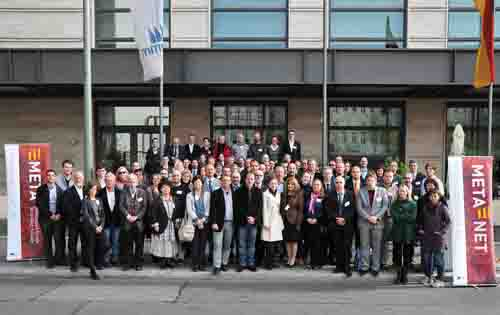
\includegraphics[width=\textwidth]{../_media/meta-net_team.jpg}
  \caption{Takmer 100 odborníkov na jazykové technológie – predstavitelia krajín a jazykov META-NET-u – prediskutovalo a sformulovalo kľučové východiská a odkazy série bielych kníh na stretnutí META-NET-u 21. a 22. októbra v Berlíne, Nemecko. --- \textcolor{grey1}{About 100 language technology experts -- representatives of the countries and languages represented in META-NET -- discussed and finalised the key results and messages of the White Paper Series at a META-NET meeting in Berlin, Germany, on October 21/22, 2011.}}
  \medskip
  \colorrule{grey3}{\textwidth}{1.5pt}
\end{figure*}

\cleardoublepage
\bsection[Séria bielych kníh META-NET-u -- The META-NET White Paper Series]{Séria bielych kníh META-NET-u --- The META-NET\ \ \ \ \ \ White Paper Series}
\label{whitepaperseries}

\vspace*{-5mm}
\centering
  \setlength{\tabcolsep}{2em}
  \begin{tabularx}{\textwidth}{lllll} \toprule\addlinespace
  & angličtina & English & English & \\
  & baskičtina & Basque & euskara & \\
  & bulharčina & Bulgarian & български & \\
  & čeština & Czech & čeština & \\
  & dánčina & Danish & dansk & \\
  & estónčina & Estonian & eesti & \\
  & fínčina & Finnish & suomi & \\
  & francúzština & French & français & \\
  & galícijčina & Galician & galego & \\
  & gréčtina & Greek & ελληνικά & \\
  & holandčina & Dutch & Nederlands & \\
  & chorvátčina & Croatian & hrvatski & \\
  & islandčina & Icelandic & íslenska & \\
  & írčina & Irish & Gaeilge & \\
  & katalánčina & Catalan & català & \\
  & litovčina & Lithuanian & lietuvių kalba & \\ 
  & lotyština & Latvian & latviešu valoda & \\
  & maďarčina & Hungarian & magyar & \\ 
  & maltčina & Maltese & Malti & \\
  & nemčina & German & Deutsch & \\
  & nórčina (bokmål)  & Norwegian Bokmål & bokmål & \\
  & nórčina (nynorsk) & Norwegian Nynorsk & nynorsk & \\
  & poľština & Polish & polski & \\
  & portugalčina & Portuguese & português & \\
  & rumunčina & Romanian & română & \\
  & slovenčina & Slovak & slovenčina & \\
  & slovinčina & Slovene & slovenščina & \\
  & srbčina & Serbian & српски & \\
  & španielčina & Spanish & español & \\
  & švédčina & Swedish & svenska & \\
  & taliančina & Italian & italiano & \\ \addlinespace \bottomrule
\end{tabularx}

